%!TEX root = ../my_thesis.tex
\section[Fits to the $B^0$ invariant mass]{Fits to the \boldmath{$B^0$} invariant mass}
\label{sec:massfit}

The \emph{sPlot} technique~\cite{sPlot} is applied in order to statistically
isolate the signal contribution for the subsequent decay time fit. The $\Dmp\pipm$ invariant
mass, where the $\Dmp$ mass is constrained to its known value in order to improve
the mass resolution, is adopted as discriminating observable thanks to its small
correlation with the $\Bz$ decay time (see Appendix \ref{app:invariantMassFit}).

In a first step, a binned extended maximum likelihood fit (``Fit A'') is
performed in order to define the PDFs describing the  signal and background
components. The choice of a binned fit is justified by the very high statistics
of the data sample. The invariant mass range of the fit is $[5090,6000]\mevcc$.
Only tagged candidates are considered, \ie~candidates with at least one nonzero tagging
decision from the OS or SS taggers. The reason for this is that untagged candidates do
not contribute to the sensitivity on the \CP~coefficients.
The fit is performed simultaneously on the pion and kaon samples (see
Sec.~\ref{sec:preselection}). This approach is adopted in order to control the
contamination from the $\Bz\to\Dm\Kp$  background  in the pion sample. The number of
$\Bz\to DX$ candidates in the $Y$ sample (with $X,Y=\pi,K$), $N^{Y}_{\Bz\to
DX}$, can be defined via the following relations:
%
\begin{equation}
	\label{eq:Bd2DPiconstr}
	\begin{split}
		N^{K}_{\Bz\to D\pi}
		&= \frac{\epsilon_{\rm PID}(\Bz\to D\pi)_{K}}{\epsilon_{\rm PID}(\Bz\to D\pi)_{\pi}}\times N^{\pi}_{\Bz\to D\pi}  = \frac{1-\epsilon_{\rm PID}(\Bz\to D\pi)_{\pi}}{\epsilon_{\rm PID}(\Bz\to D\pi)_{\pi}}\times N^{\pi}_{\Bz\to D\pi},
	\end{split}
\end{equation}
\begin{equation}
	\label{eq:Bd2DKconstr}
	\begin{split}
		N^{\pi}_{\Bz\to DK}
		&= \frac{\epsilon_{\rm PID}(\Bz\to DK)_{\pi}}{\epsilon_{\rm PID}(\Bz\to DK)_{K}}\times N^{K}_{\Bz\to DK} = \frac{1-\epsilon_{\rm PID}(\Bz\to DK)_{K}}{\epsilon_{\rm PID}(\Bz\to DK)_{K}}\times N^{K}_{\Bz\to DK}.
	\end{split}
\end{equation}
%
The quantities $\epsilon_{\rm PID}(\Bz\to DX)_{Y}$ are the fractions of true
$\Bz\to DX$ decays that are selected in the $Y$ sample by applying the
corresponding $\PIDK$ cut. These fractions (or efficiencies) are estimated on $\Bz\to
\Dmp\pipm$ and $\Bz\to\Dm\Kp$ MC samples where the $\PIDK$ distributions are
resampled from calibration data, as described in Sec.~\ref{sec:pid}. 
A systematic uncertainty for these efficiencies is estimated by taking the largest
discrepancy between the nominal value and the result obtained with the narrow and wide
binning schemes introduced in Sec.~\ref{sec:pid}.
The results
of these estimations are reported in Table~\ref{tab:pideff}.

\begin{table}[t]
	\begin{center}
		\caption{Fractions of true $\Bz\to\Dmp\pipm$ and $\Bz\to\Dm\Kp$ decays that are
		selected in the $\pi$ or $K$ sample.}
		\begin{tabular}{ccc}
			\toprule
			Decay & $\PIDK$ requirement & fraction\\
			\midrule
			$\Bz\to\Dmp\pipm$ & $<5$ ($\pi$ sample) & $0.9790\pm0.0040(\rm stat)\pm0.0004(\rm syst)$\\
			$\Bz\to\Dmp\pipm$ & $>5$ ($K$ sample) & $0.0211\pm0.0005(\rm stat)\pm0.0004(\rm syst)$\\
			\midrule
			$\Bz\to\Dm\Kp$ & $<5$ ($\pi$ sample) & $0.373\pm0.005(\rm stat)\pm0.008(\rm syst)$\\
			$\Bz\to\Dm\Kp$ & $>5$ ($K$ sample) & $0.627\pm0.007(\rm stat)\pm0.010(\rm syst)$\\
			\bottomrule
		\end{tabular}
		\label{tab:pideff}
	\end{center}
\end{table}

Finally, an unbinned extended maximum likelihood fit (``Fit B'') is performed on
data using the reduced mass interval $[5220,5600]\mevcc$ in order to extract
\emph{sWeights}. In this second fit, all the parameters are fixed to the values
found in Fit A, except for the signal and total background yields. The reduced mass window avoids
diluting the \emph{sWeights} with background candidates having an invariant mass falling outside this window. This has
the added advantage of reducing the dataset size used in the decay time fit.

%===============================================================================
\subsection{Probability density functions}
\label{sec:pdf}

The PDFs used to describe both the pion and kaon sample
components in Fit A are first estimated on MC samples. The parameters of the
combinatorial background PDFs are instead determined directly from data. The PDFs
used for the pion sample are:
\begin{itemize}[noitemsep,topsep=0pt]
	\item $\Bz\to\Dmp\pipm$: sum of a double-sided Hypatia~\cite{Hypatia} and a Johnson SU~\cite{JohnsonSU} function (${\rm PDF}^{\pi}_{\Bz\to D\pi}$).
	\item $\Bz\to\Dm\Kp$: double-sided Hypatia function (${\rm PDF}^{\pi}_{\Bz\to DK}$).
	\item $\Bz\to\Dmp\rho^\pm$: Johnson SU function (${\rm PDF}^{\pi}_{\Bz\to D\rho}$).
	\item $\Bz\to D^{*\mp}\pipm$: sum of a single-sided Crystal Ball function~\cite{Skwarnicki:1986xj} and a Gaussian function (${\rm PDF}^{\pi}_{\Bz\to \Dst\pi}$).
	\item Background: sum of an exponential function and a constant offset.
\end{itemize}
For the kaon sample they are:
\begin{itemize}[noitemsep,topsep=0pt]
	\item $\Bz\to\Dmp\pipm$: double-sided Hypatia function (${\rm PDF}^{K}_{\Bz\to D\pi}$).
	\item $\Bz\to\Dm\Kp$: single-sided Hypatia function (${\rm PDF}^{K}_{\Bz\to DK}$).
	\item $\Bz\to\Dmp\rho^\pm$: double Gaussian function (${\rm PDF}^{K}_{\Bz\to D\rho}$).
	\item $\Bz\to\Dmp K^{*\pm}$: Gaussian function (${\rm PDF}^{K}_{\Bz\to D\Kst}$).
	\item Background: sum of an exponential function and a constant offset.
\end{itemize}
The definitions of all the PDFs listed above are reported in
Appendix~\ref{app:pdfsdef}. The fits to the MC samples are shown in
Figs.~\ref{fig:MCPisample} and~\ref{fig:MCKsample}. The parameters obtained from these fits that are then fixed in the data fits are listed in Tables~\ref{tab:FitAfixedPisample} and~\ref{tab:FitAfixedKsample}.

\begin{figure}[t]
	\centering
	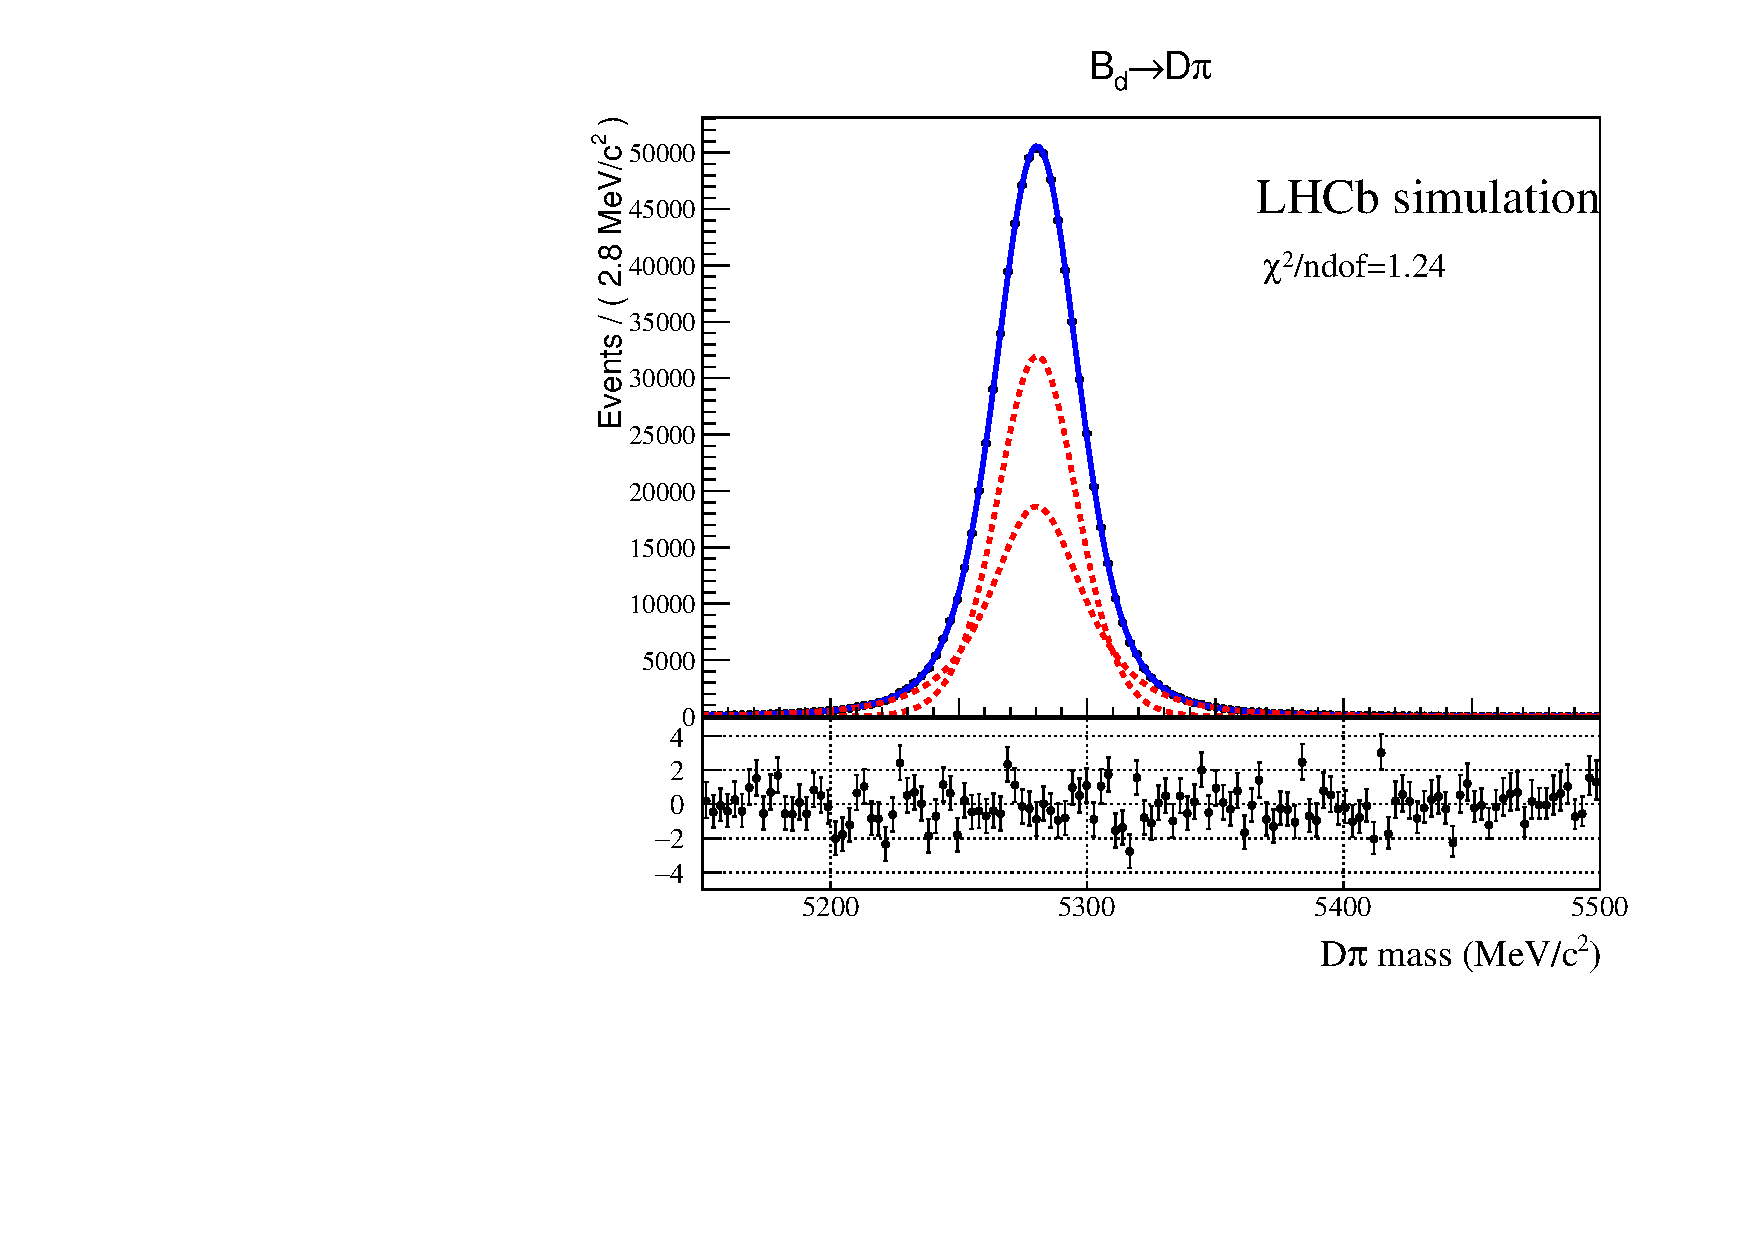
\includegraphics[width=0.45\linewidth]{03Massfit/figs/Template_combData_Signal_both_kpipi_2012_Bd2DPiHypo_BeautyMass_binned.pdf}
	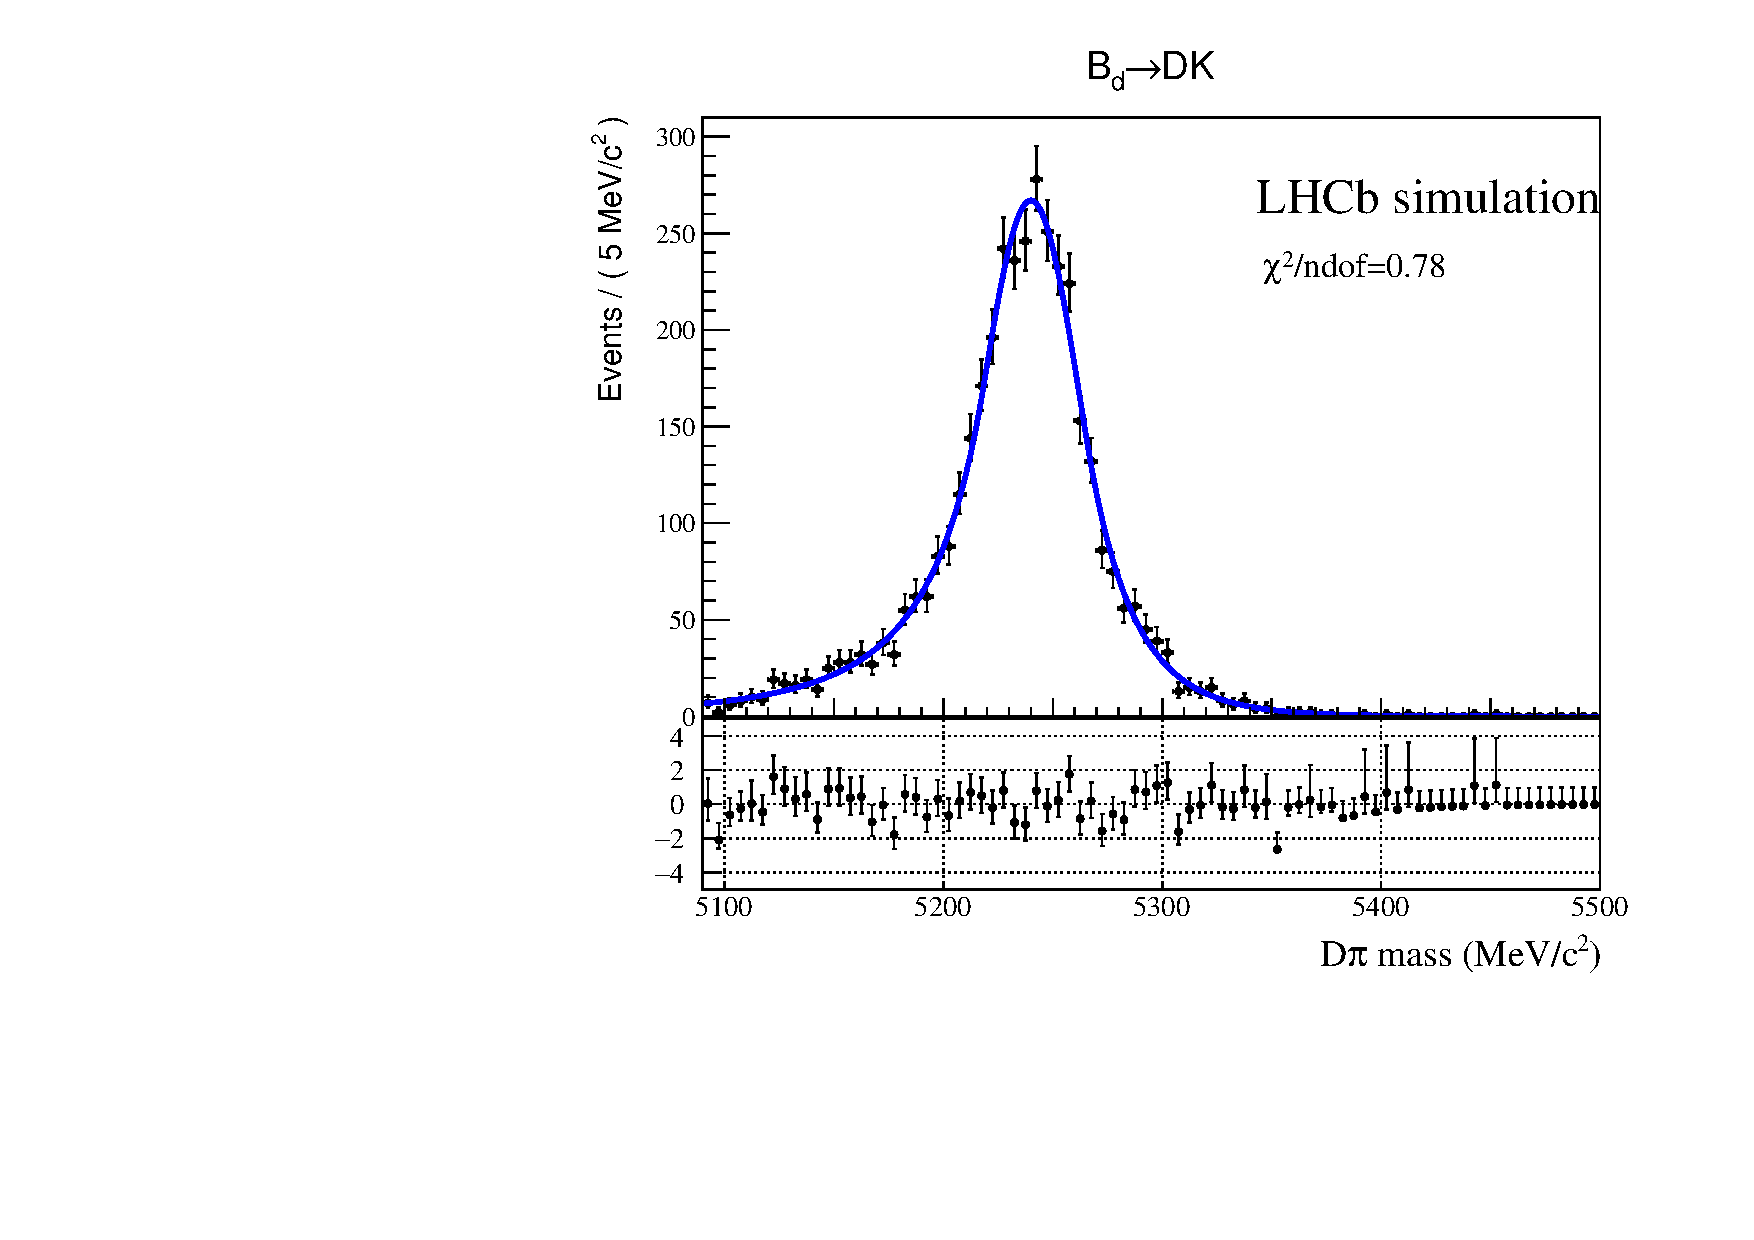
\includegraphics[width=0.45\linewidth]{03Massfit/figs/Template_combData_Bd2DK_both_2012_Bd2DPiHypo_BeautyMass.pdf} \\
	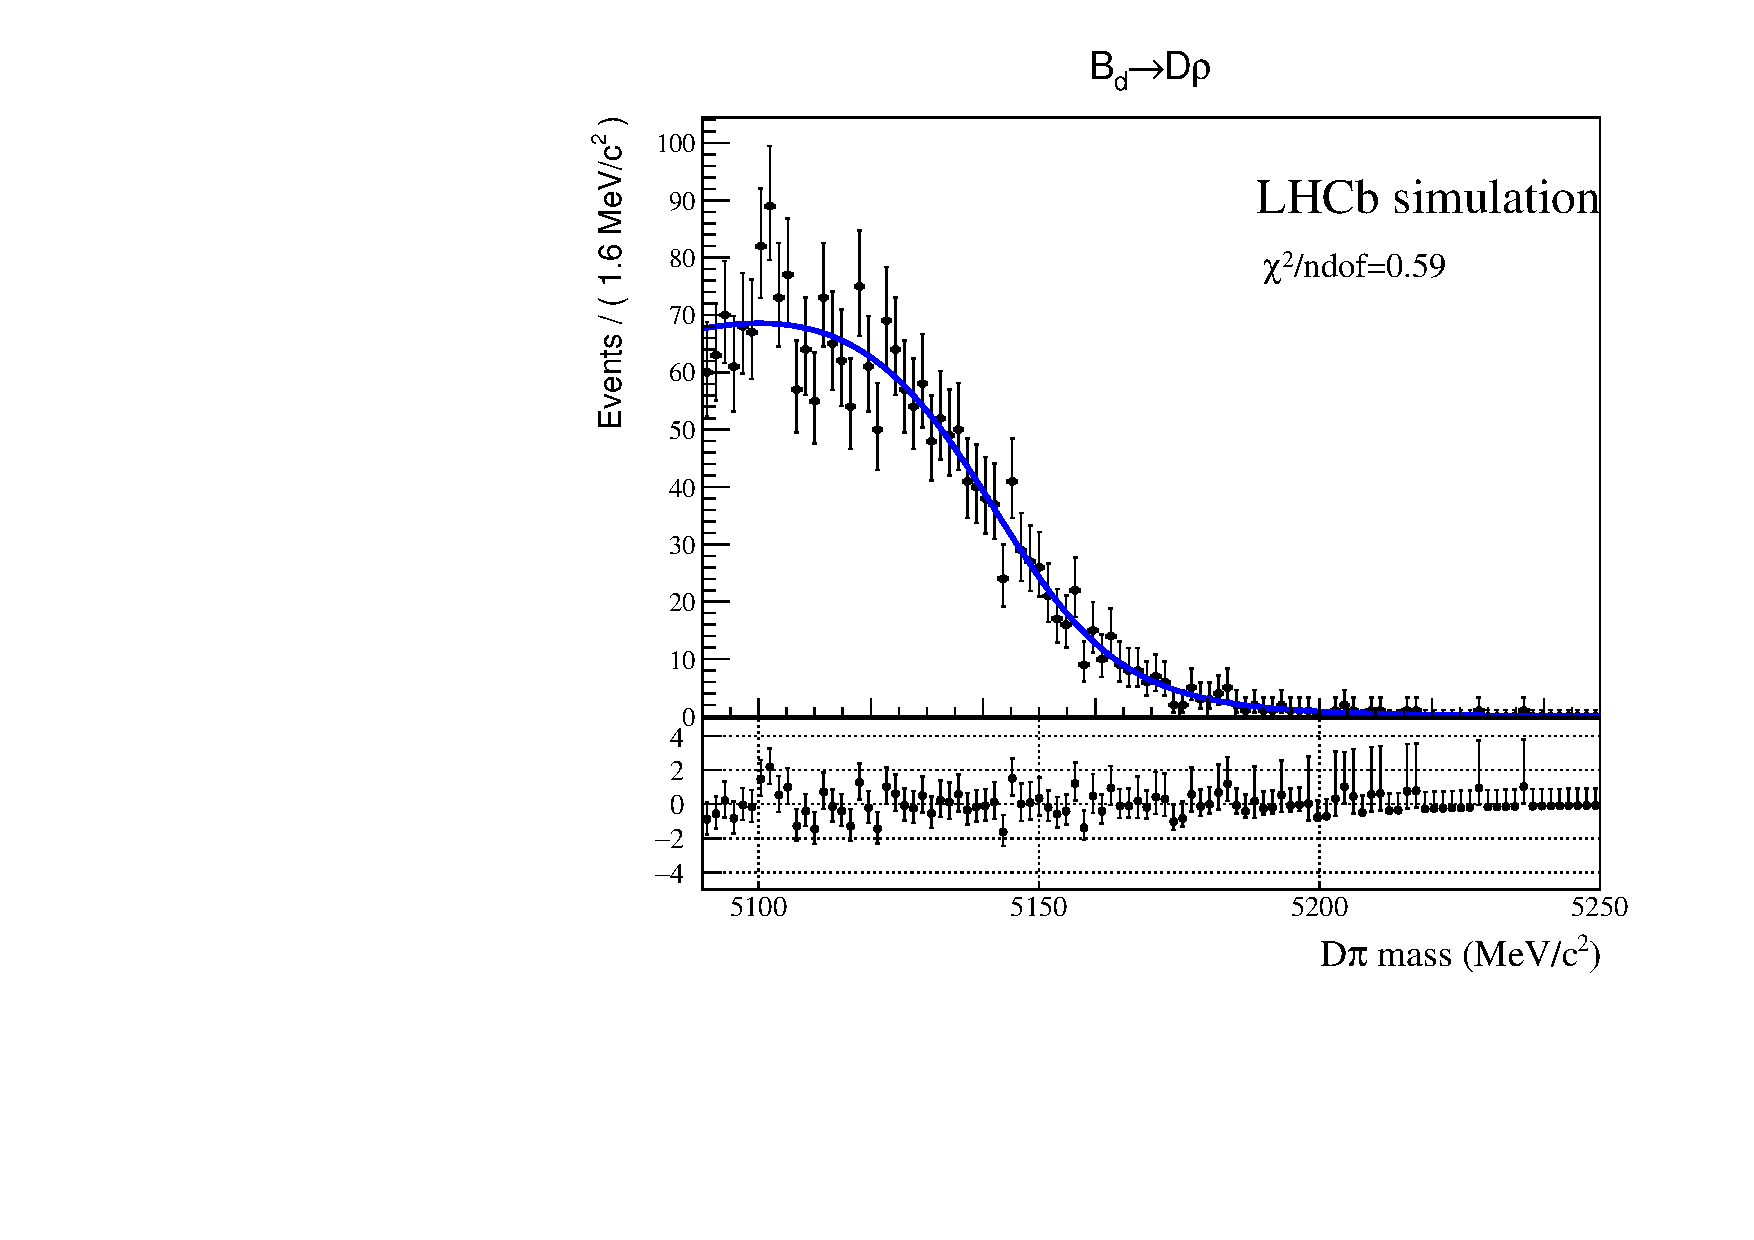
\includegraphics[width=0.45\linewidth]{03Massfit/figs/Template_combData_Bd2DRho_both_2012_Bd2DPiHypo_BeautyMass.pdf}
	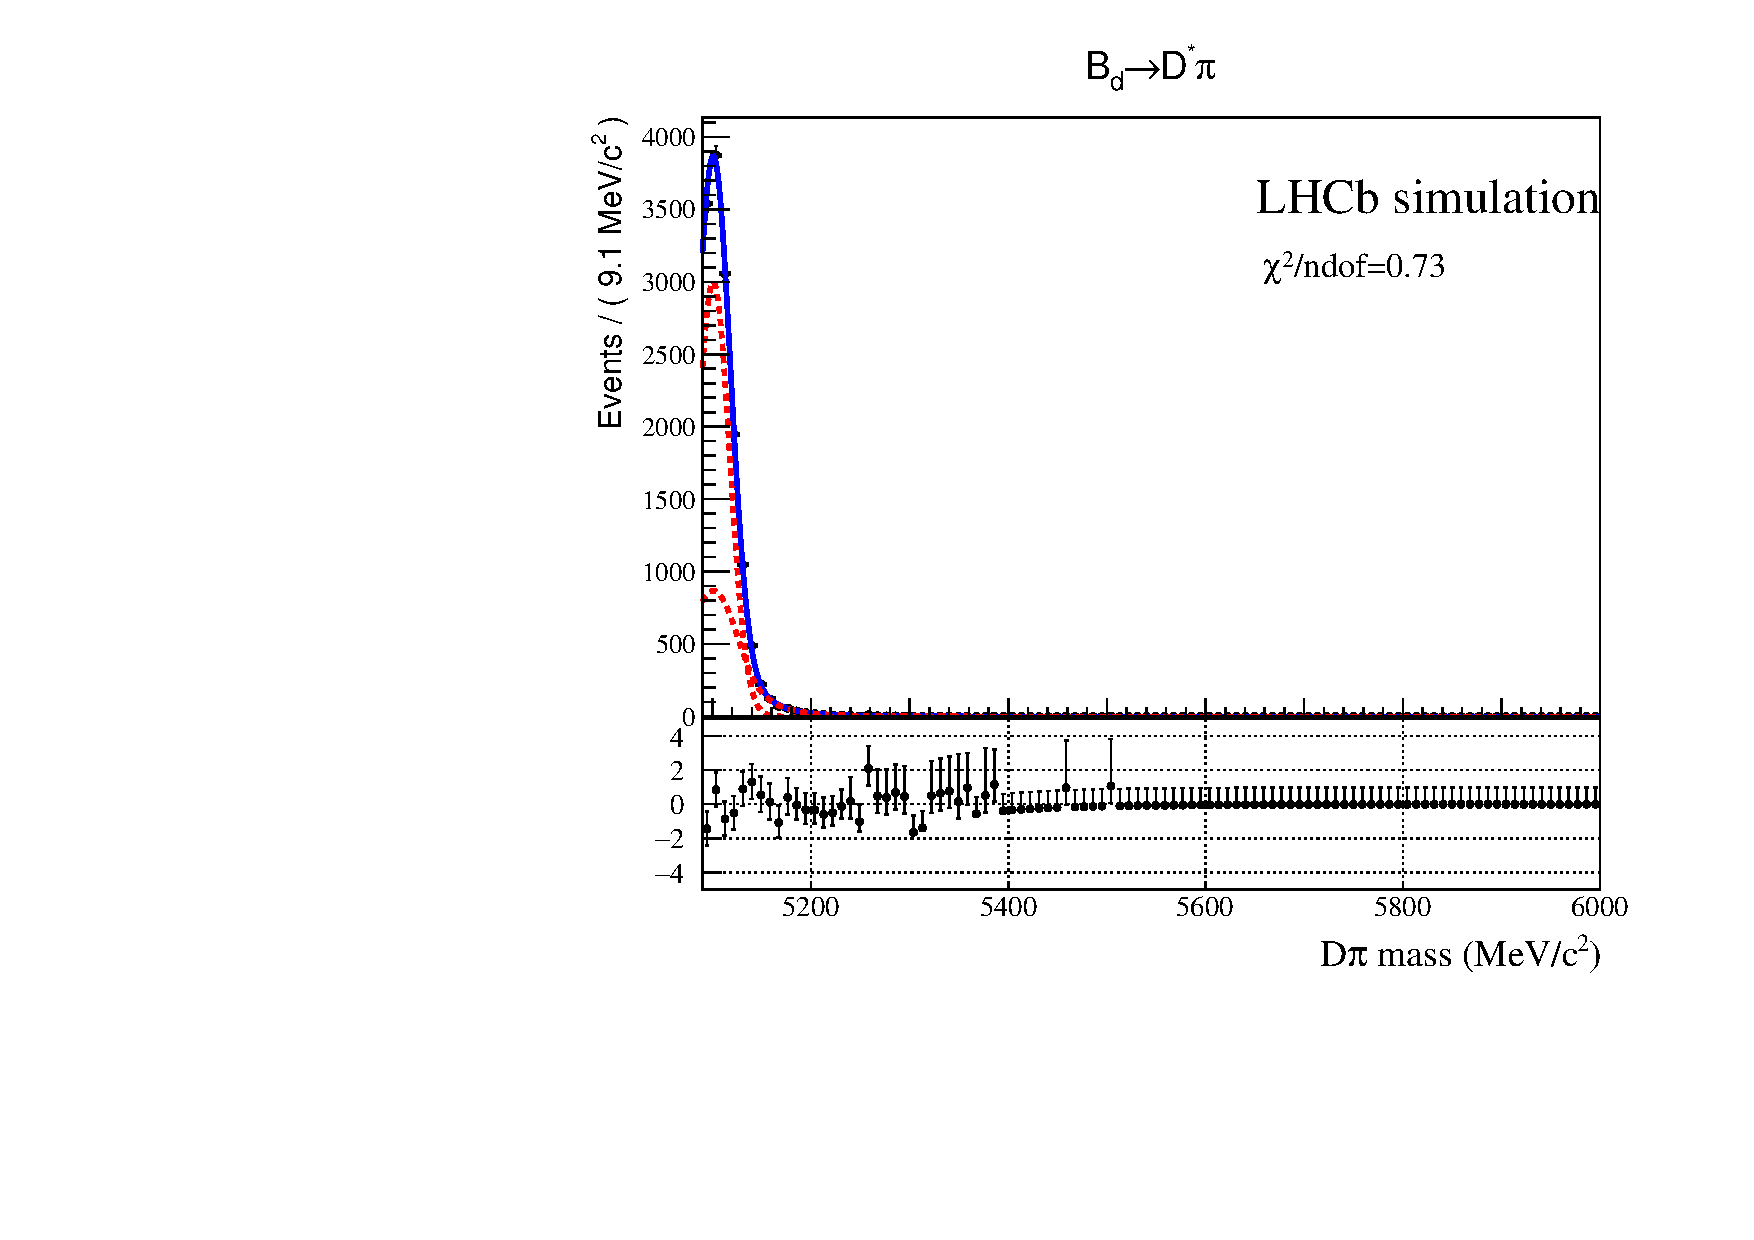
\includegraphics[width=0.45\linewidth]{03Massfit/figs/Template_combData_Bd2DstPi_both_2012_Bd2DPiHypo_BeautyMass.pdf} \\
        \vspace{-2mm}
	\caption{$\Dmp\pipm$ mass distributions of MC samples of $\Bz\to\Dmp\pipm$ (top left), $\Bz\to\Dm\Kp$ (top right),
          $\Bz\to\Dmp\rho^\pm$ (bottom left) and $\Bz\to D^{*\mp}\pipm$ (bottom right) events passing the $\Bz\to\Dmp\pipm$
          selection, with fits superimposed.}
	\label{fig:MCPisample}
\end{figure}

\begin{figure}[t]
	\centering
	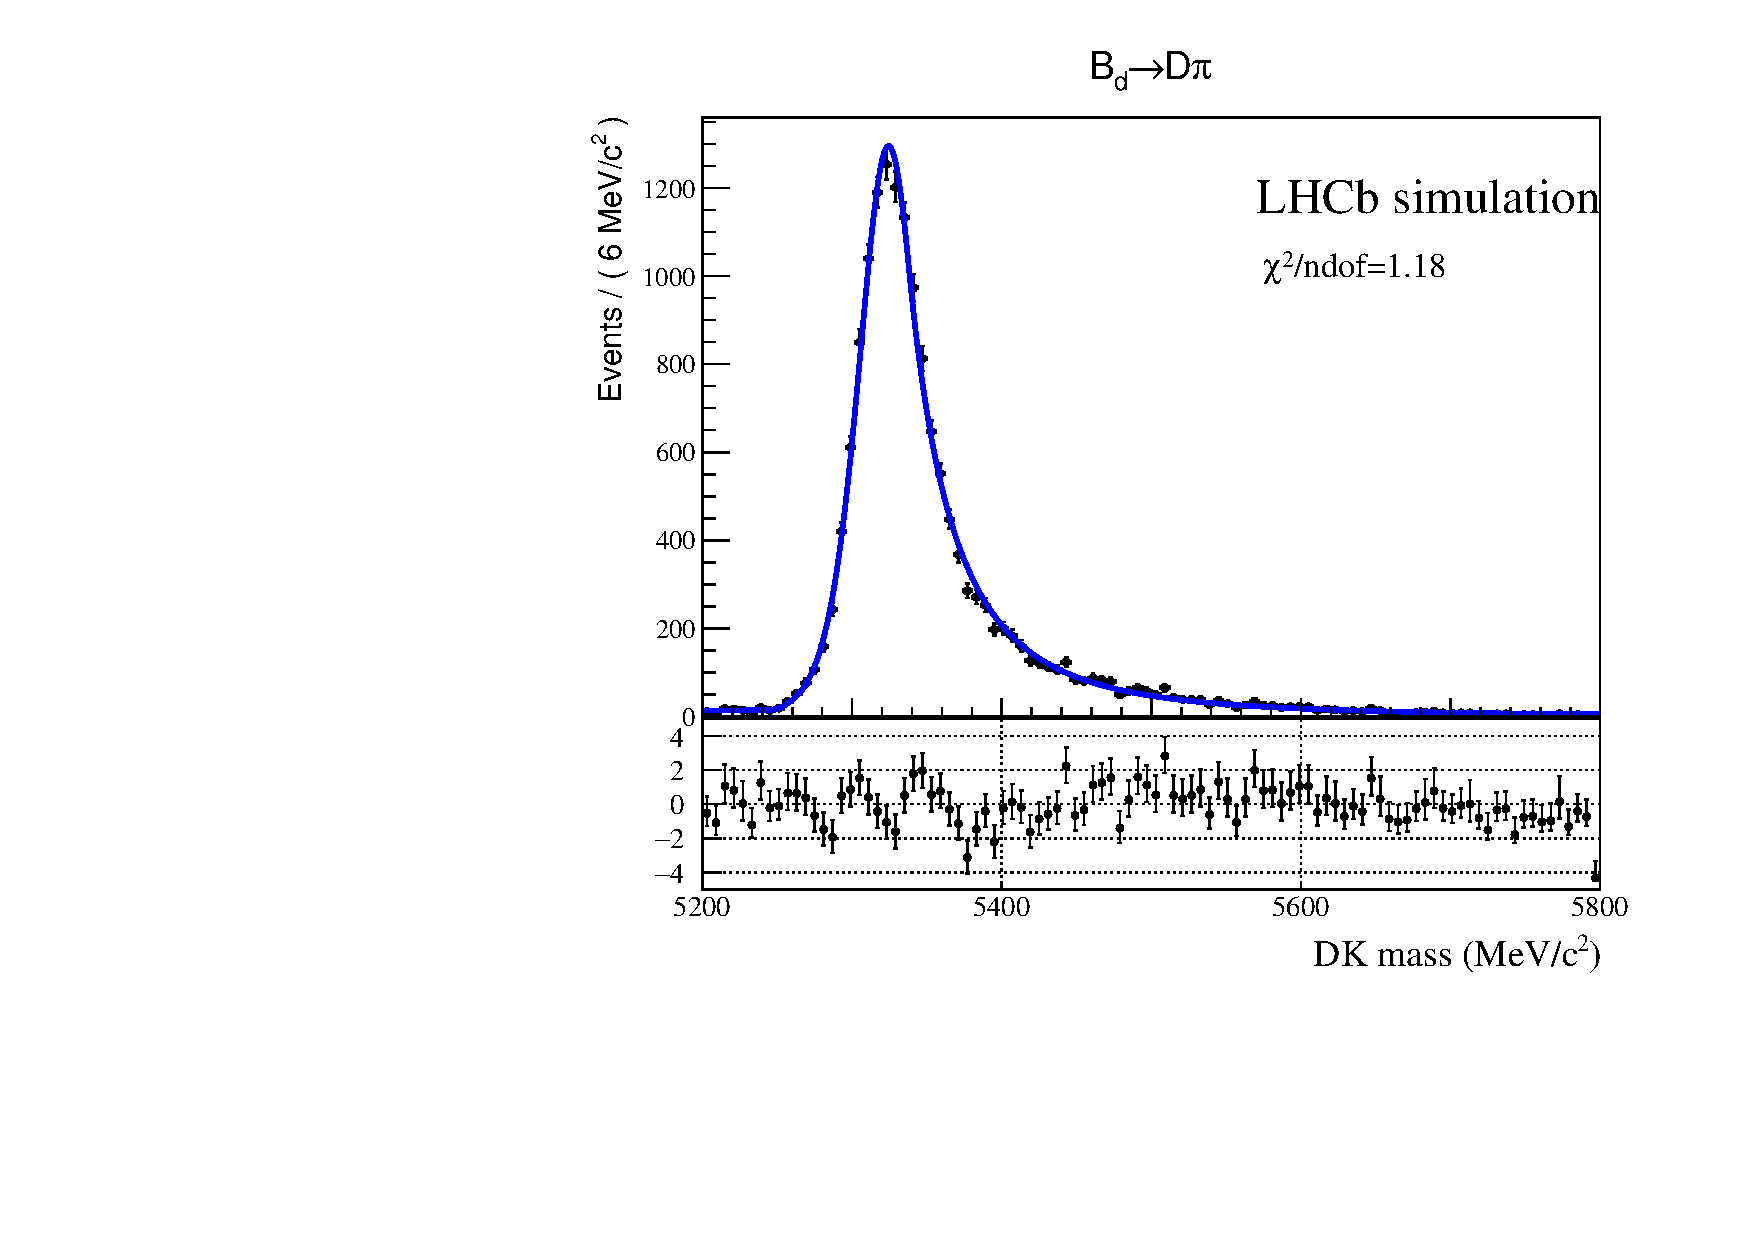
\includegraphics[width=0.45\linewidth]{03Massfit/figs/Template_combData_Signal_both_kpipi_2012_Bd2DKHypo_BeautyMass_binned.pdf}
	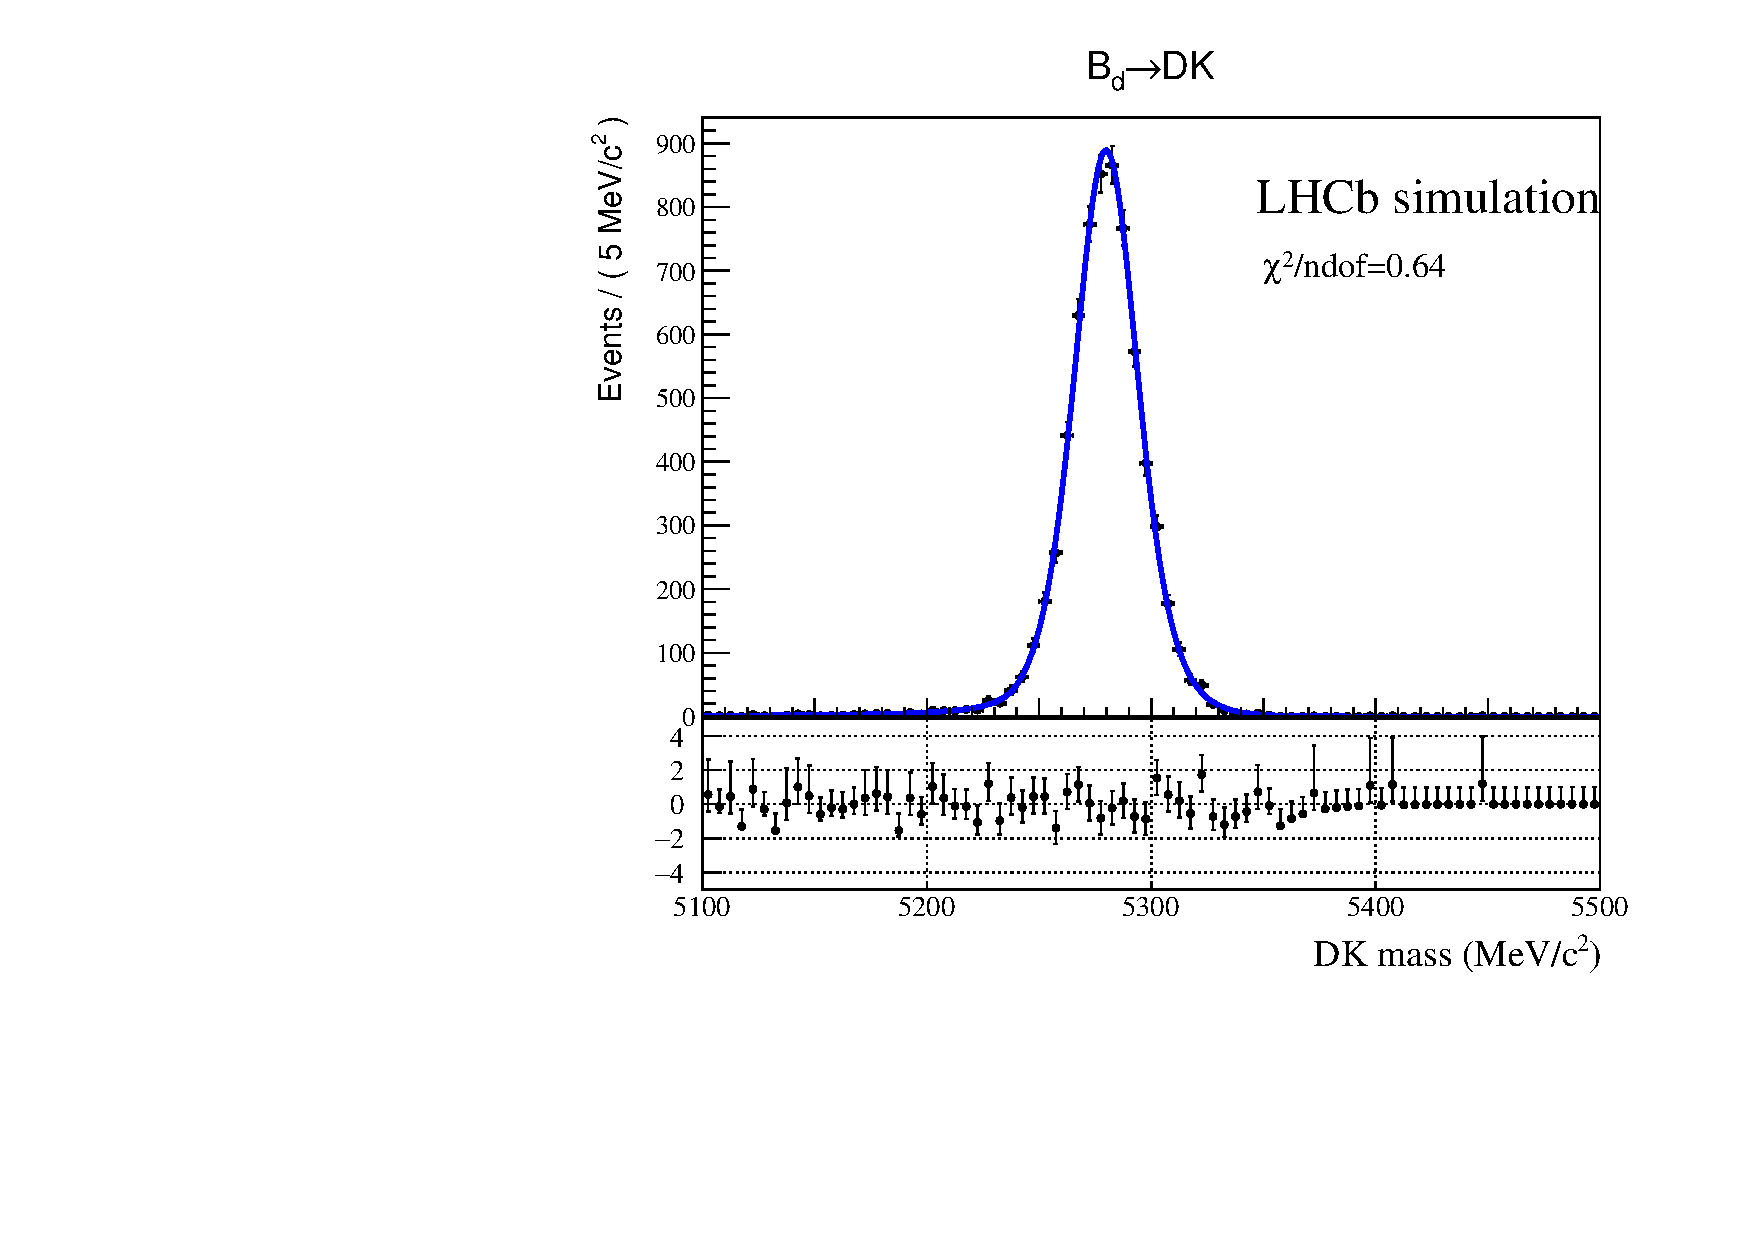
\includegraphics[width=0.45\linewidth]{03Massfit/figs/Template_combData_Bd2DK_both_2012_Bd2DKHypo_BeautyMass.pdf} \\
	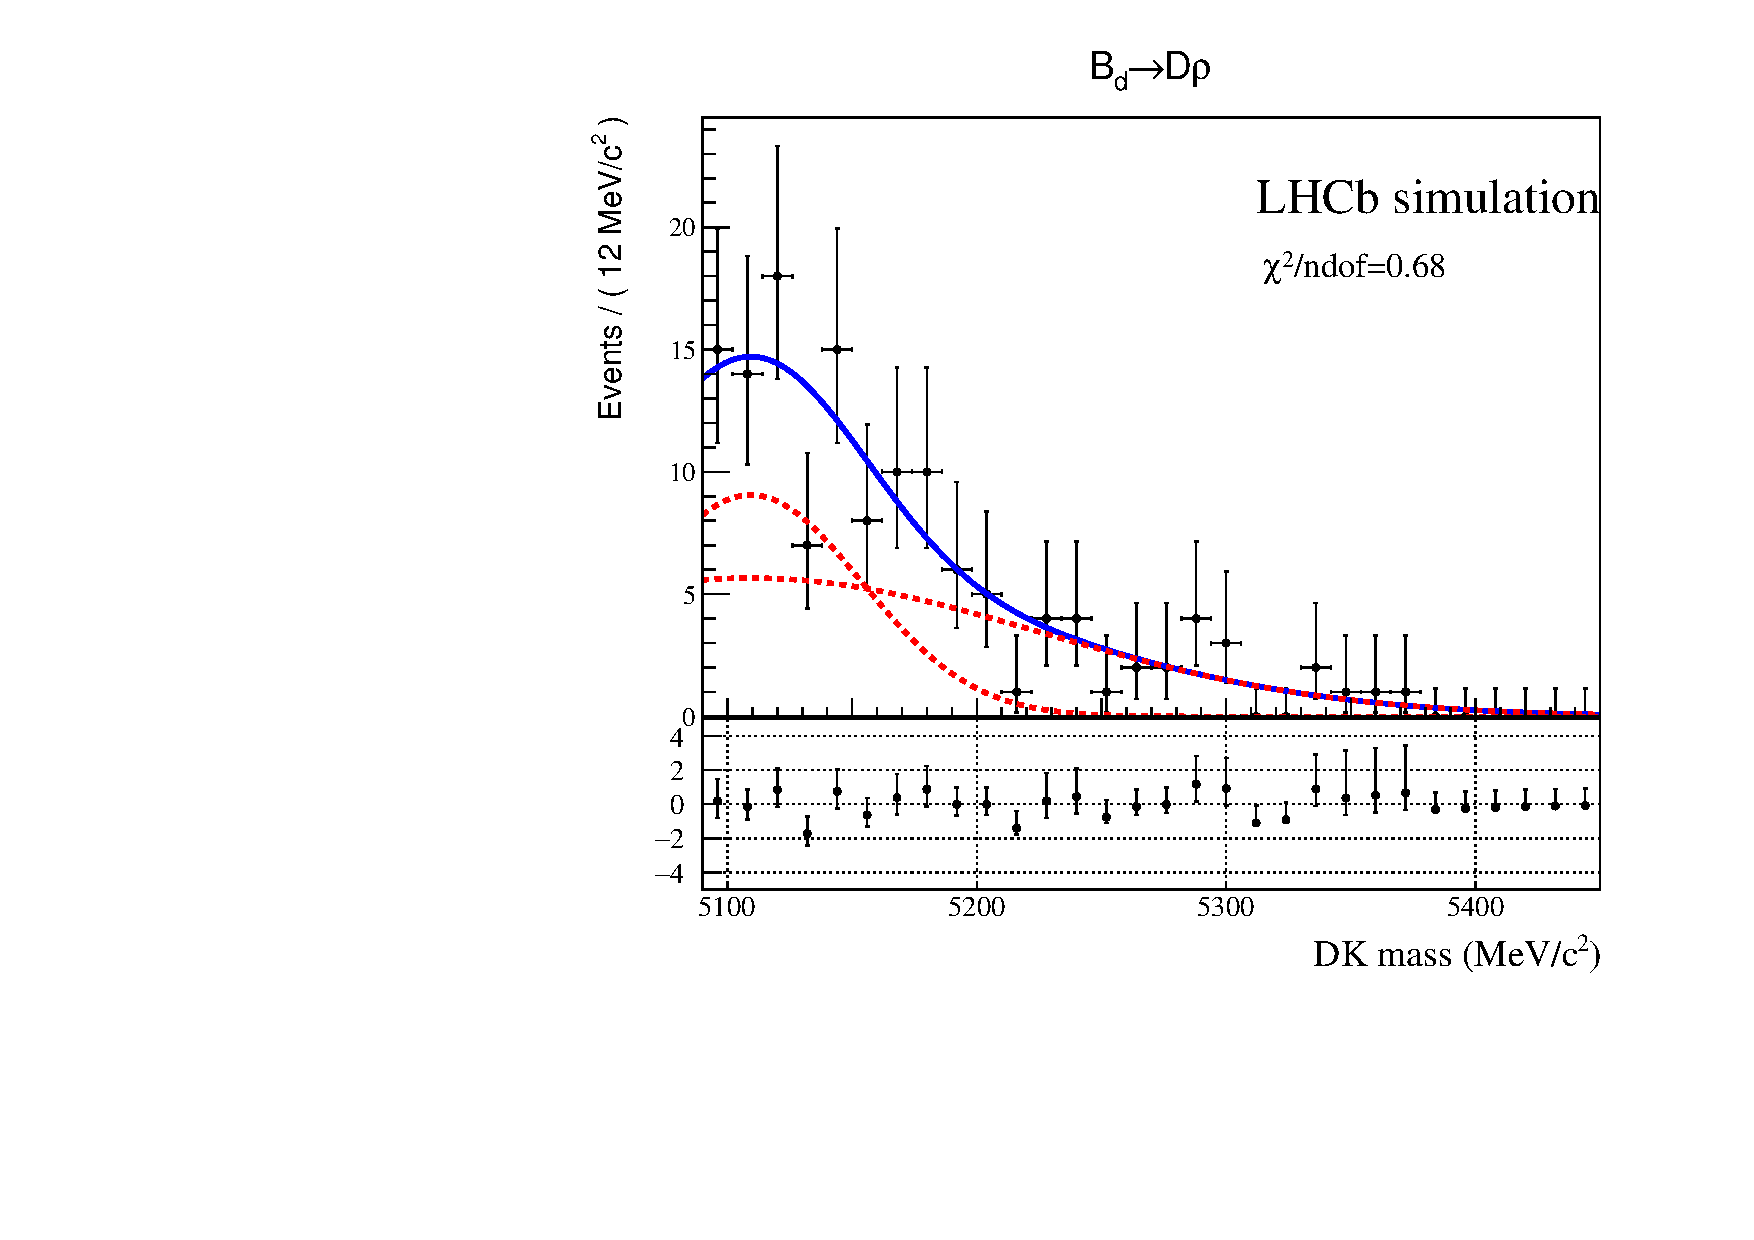
\includegraphics[width=0.45\linewidth]{03Massfit/figs/Template_combData_Bd2DRho_both_2012_Bd2DKHypo_BeautyMass.pdf}
	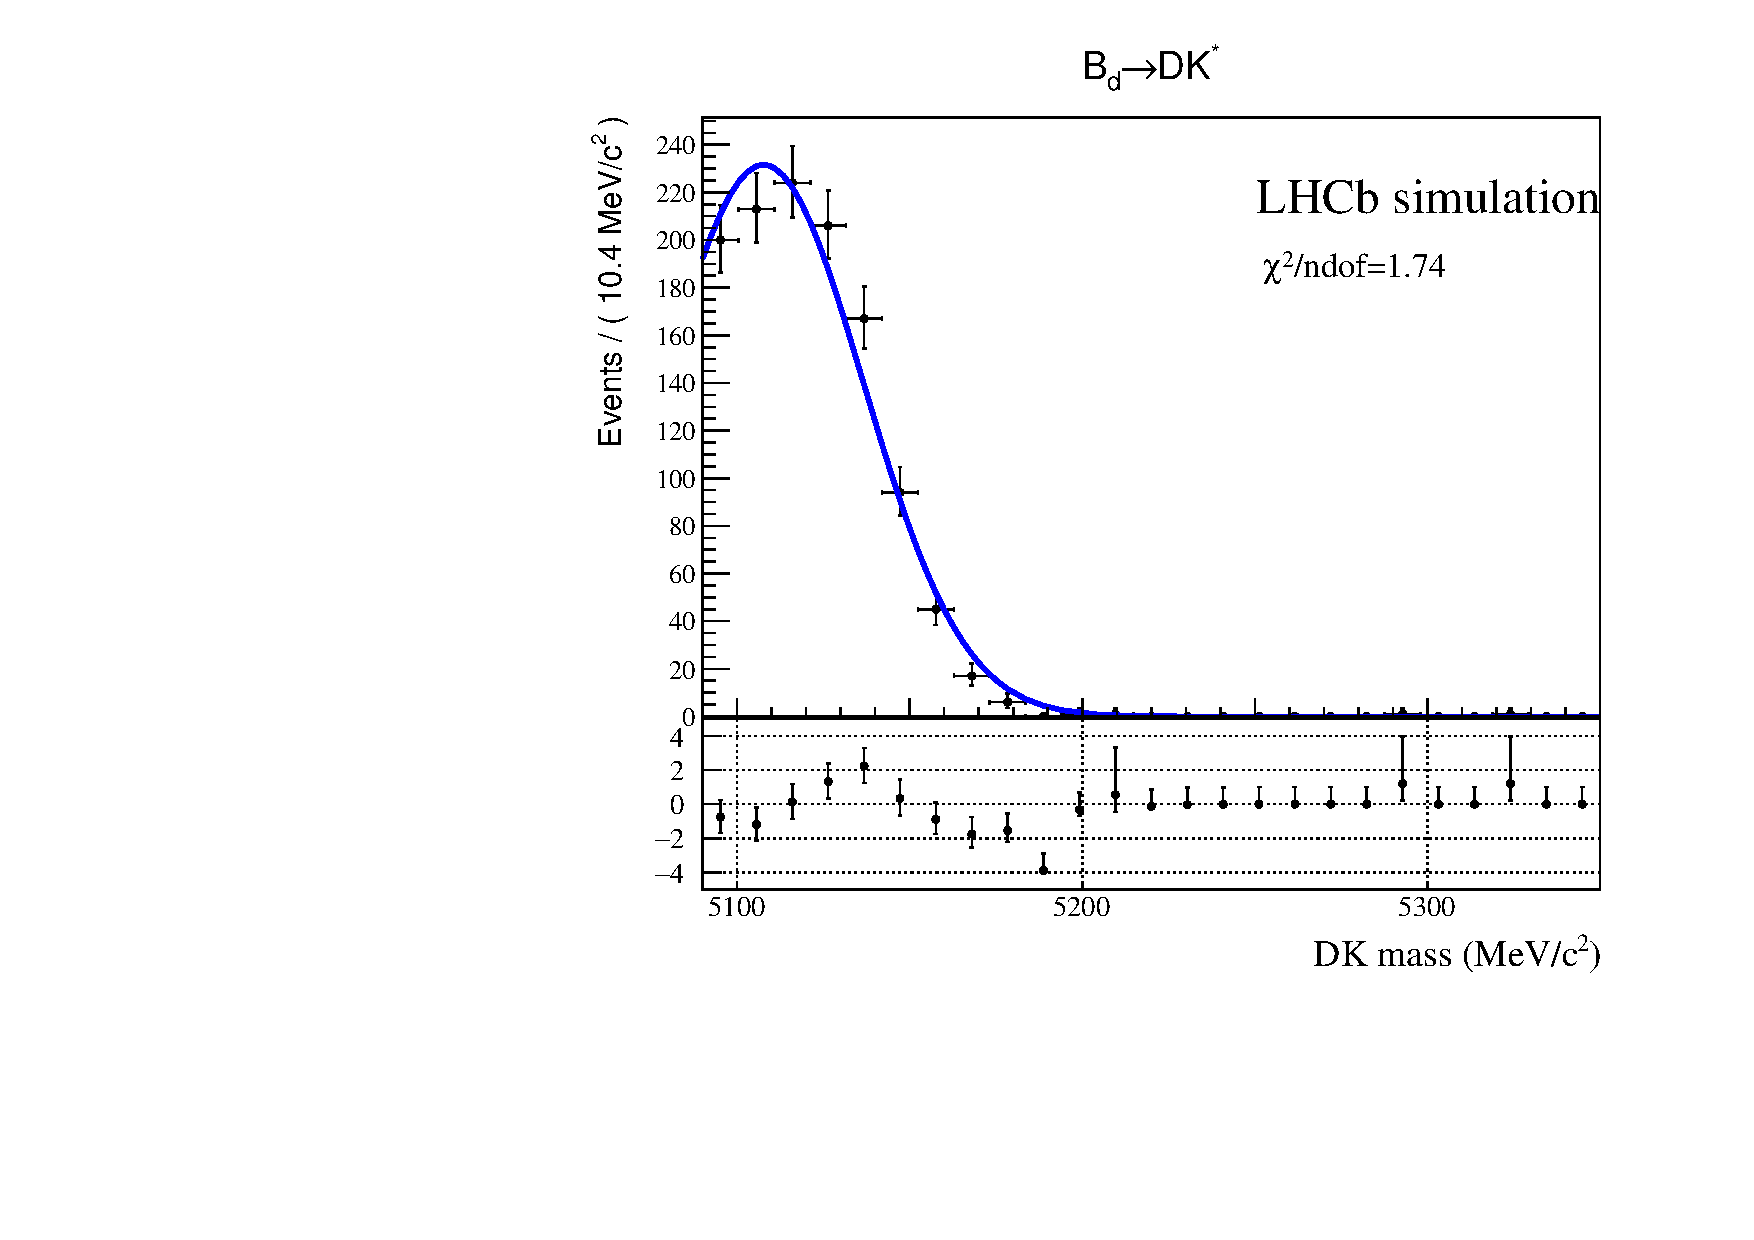
\includegraphics[width=0.45\linewidth]{03Massfit/figs/Template_combData_Bd2DKst_both_2012_Bd2DKHypo_BeautyMass.pdf} \\
	\vspace{-2mm}
        \caption{$\Dmp\Kpm$ mass distributions of MC samples of $\Bz\to\Dmp\pipm$ (top left), $\Bz\to\Dm\Kp$ (top right),
          $\Bz\to\Dmp\rho^\pm$ (bottom left) and $\Bz\to D^{-}K^{*+}$ (bottom right) events passing the $\Bz\to\Dmp\pipm$
          selection, with fits superimposed.}
	\label{fig:MCKsample}
\end{figure}

%-------------------------------------------------------------------------------
\subsection{Fit to data}
\label{sec:DataMassFit}

In order to perform Fit A, two fitting functions are defined:
\begin{equation}
	\label{eq:PiSamplePDF}
	\begin{split}
		f_{\pi}(m) &= N^{\pi}_{\Bz\to D\pi}{\rm{PDF}}^{\pi}_{\Bz\to D\pi} + N^{\pi}_{\Bz\to DK}{\rm{PDF}}^{\pi}_{\Bz\to DK} \\
		& + N^{\pi}_{\Bz\to \Dst\pi}{\rm{PDF}}^{\pi}_{\Bz\to \Dst\pi} + N^{\pi}_{\Bz\to D\rho}{\rm{PDF}}^{\pi}_{\Bz\to D\rho} \\
		& + N^{\pi}_{\rm comb}{\rm{PDF}}^{\pi}_{\rm comb},
	\end{split}
\end{equation}
\begin{equation}
	\label{eq:KSamplePDF}
	\begin{split}
		f_{K}(m) &= N^{K}_{\Bz\to DK}{\rm{PDF}}^{K}_{\Bz\to DK} + N^{K}_{\Bz\to D\pi}{\rm{PDF}}^{K}_{\Bz\to D\pi} \\
		& +N^{K}_{\Bz\to D\Kst}{\rm{PDF}}^{K}_{\Bz\to D\Kst} + N^{K}_{\Bz\to D\rho}{\rm{PDF}}^{K}_{\Bz\to D\rho} \\
		& +N^{K}_{\rm comb}{\rm{PDF}}^{K}_{\rm comb}.
	\end{split}
\end{equation}
Two extended likelihood functions are defined using data and PDFs related to both samples:
\begin{align}
	\mathcal L_{x} &= \frac{e^{-N_{x,\rm exp}}\left(N_{x,\rm exp}\right)^{N_{x,\rm obs}}}{N_{x,\rm obs}!} \prod\limits_{i=1}^{N_{x,\rm obs}}\frac{f_{x}(m_i)}{N_{x,\rm exp}}\,, & x &= \pi, K\,,
\end{align}
where $N_{\pi,\rm exp}=N^{\pi}_{\Bz\to D\pi}+N^{\pi}_{\Bz\to DK}+N^{\pi}_{\Bz\to \Dst\pi}+N^{\pi}_{\Bz\to D\rho}+N^{\pi}_{\rm comb}$,
$N_{K,\rm exp}=N^{K}_{\Bz\to DK}+N^{K}_{\Bz\to D\pi}+N^{K}_{\Bz\to D\Kst}+N^{K}_{\Bz\to D\rho}+N^{K}_{\rm comb}$, and 
$N_{x,\rm obs}$ is the number of observed candidates in the $x$ sample.
The product $\mathcal L_{\pi}\mathcal L_{K}$ is maximised during the fit.

The following strategy is adopted to perform Fit A:
\begin{itemize}[noitemsep,topsep=0pt]
	\item The mean and width parameters ($\mu^{\pi}_{\Bz\to D\pi}$,
		$\sigma H^{\pi}_{\Bz\to D\pi}$, $\sigma J^{\pi}_{\Bz\to D\pi}$, $\mu^{K}_{\Bz\to DK}$, $\sigma^{K}_{\Bz\to DK}$)
		of ${\rm{PDF}}^{\pi}_{\Bz\to D\pi}$ and ${\rm PDF}^{K}_{\Bz\to DK}$ are floated in the fit.
	\item The tail parameters ($a1^{\pi}_{\Bz\to D\pi}$, $a2^{\pi}_{\Bz\to D\pi}$,
		$n1^{\pi}_{\Bz\to D\pi}$, $n2^{\pi}_{\Bz\to D\pi}$) of
		${\rm{PDF}}^{\pi}_{\Bz\to D\pi}$ are constrained in the following way:
		$a1^{\pi}_{\Bz\to D\pi}$, $a2^{\pi}_{\Bz\to D\pi}$ are set to the values
		found on MC and both multiplied by a floating scale factor
		$sa^{\pi}_{\Bz\to D\pi}$; the same constraint is applied to
		$n1^{\pi}_{\Bz\to D\pi}$ and $n2^{\pi}_{\Bz\to D\pi}$, where the scale
		factor is labelled as $sn^{\pi}_{\Bz\to D\pi}$.
	\item The yield parameters $N^{K}_{\Bz\to D\pi}$ and $N^{\pi}_{\Bz\to DK}$ are
		constrained according to Eqs.~\ref{eq:Bd2DPiconstr} and \ref{eq:Bd2DKconstr}. The
		efficiencies $\epsilon_{\rm PID}(\Bz\to D\pi)_{D\pi}$ and $\epsilon_{\rm
		PID}(\Bz\to DK)_{DK}$ are Gaussian-constrained independently in the fit,
		using the values reported in Table~\ref{tab:pideff}. 
		The yield $N^{K}_{\Bz\to D\rho}$ is fixed to be $0.92$ times
		the yield $N^{K}_{\Bz\to D\Kst}$, the latter being floated in the fit.
		This is done according to the expected $\Bz\to\Dmp\rho^\pm$ to $\Bz\to\Dmp K^{*\pm}$
		ratio in the kaon sample, which is $0.92\pm0.21$. All the other yields
		appearing in Eqs.~\ref{eq:PiSamplePDF} and
		\ref{eq:KSamplePDF} are floated in the fit.
	\item The mean parameters ($\mu^{\pi}_{\Bz\to \Dst\pi}$, $\mu^{\pi/K}_{\Bz\to
		D\rho}$) of $\rm{PDF}^{\pi}_{\Bz\to \Dst\pi}$, $\rm{PDF}^{\pi/K}_{\Bz\to
		D\rho}$, are constrained to be shifted from $\mu^{\pi}_{\Bz\to D\pi}$
		(in the $\pi$ sample) and $\mu^{K}_{\Bz\to DK}$ (in the $K$ sample) by
		the same amount found in MC. The shift of the component with
		respect to the $\Bz\to \Dmp\pipm$ ($\Bz\to \Dmp K^{\pm}$) peak in the $\pi$ ($K$) sample 
                is denoted as $\Delta\mu^{K/\pi}_{\rm comp}$. The
		mean parameters ($\mu^{K}_{\Bz\to D\Kst}$, $\mu^{\pi}_{\Bz\to DK}$,
		$\mu^{K}_{\Bz\to D\pi}$) of $\rm{PDF}^{K}_{\Bz\to D\Kst}$,
		$\rm{PDF}^{\pi}_{\Bz\to DK}$, $\rm{PDF}^{K}_{\Bz\to D\pi}$ are floated in the
		fit.
	\item The exponent parameters ($c^{\pi/K}_{\rm comb}$) and fractions
		($f^{\pi/K}_{\rm comb}$) of $\rm{PDF}^{\pi/K}_{\rm comb}$ are floated in the
		fit.
\end{itemize}

The projections of the fitted $f_{\pi}$ and $f_{K}$ in the $\Dmp\pipm$ and
$\Dmp\Kpm$ invariant mass observables (Fit A) are shown in Fig.~\ref{fig:FitA}, for 
the $\pi$ and $K$ data samples, respectively. A list of all the parameters fixed in
Fit A is given in Tables~\ref{tab:FitAfixedPisample} and \ref{tab:FitAfixedKsample}. The
fitted parameters (including yields and PID efficiencies) are listed in
Table~\ref{tab:FitAfloating}. 
%while the correlation matrix among these
%parameters in illustrated in Fig.~\ref{fig:corrFitA}.

As cross-check, the fitted yields of $\Bz\to\Dmp\Kpm$, $\Bz\to\Dmp\rho^\pm$ and $\Bz\to
D^{*\mp}\pipm$ in the pion sample are compared with the expected yields,
which are obtained, for each background,
by multiplying the fitted $\Bz\to\Dmp\pipm$ yield in the pion sample by the $f_{\rm
bkg}$ fractions given in Table~\ref{tab:expected-backgrounds}. 
These yields are reported in Table~\ref{tab:expVSfitYields}. There is 
a full agreement between expected and observed yields for the $\Bz\to\Dmp\rho^\pm$ and
$\Bz\to D^{*\mp}\pipm$ components, while the agreement for the $\Bz\to\Dmp\Kpm$ is at the level of $2.5~\sigma$.

\begin{figure}
	\begin{center}
		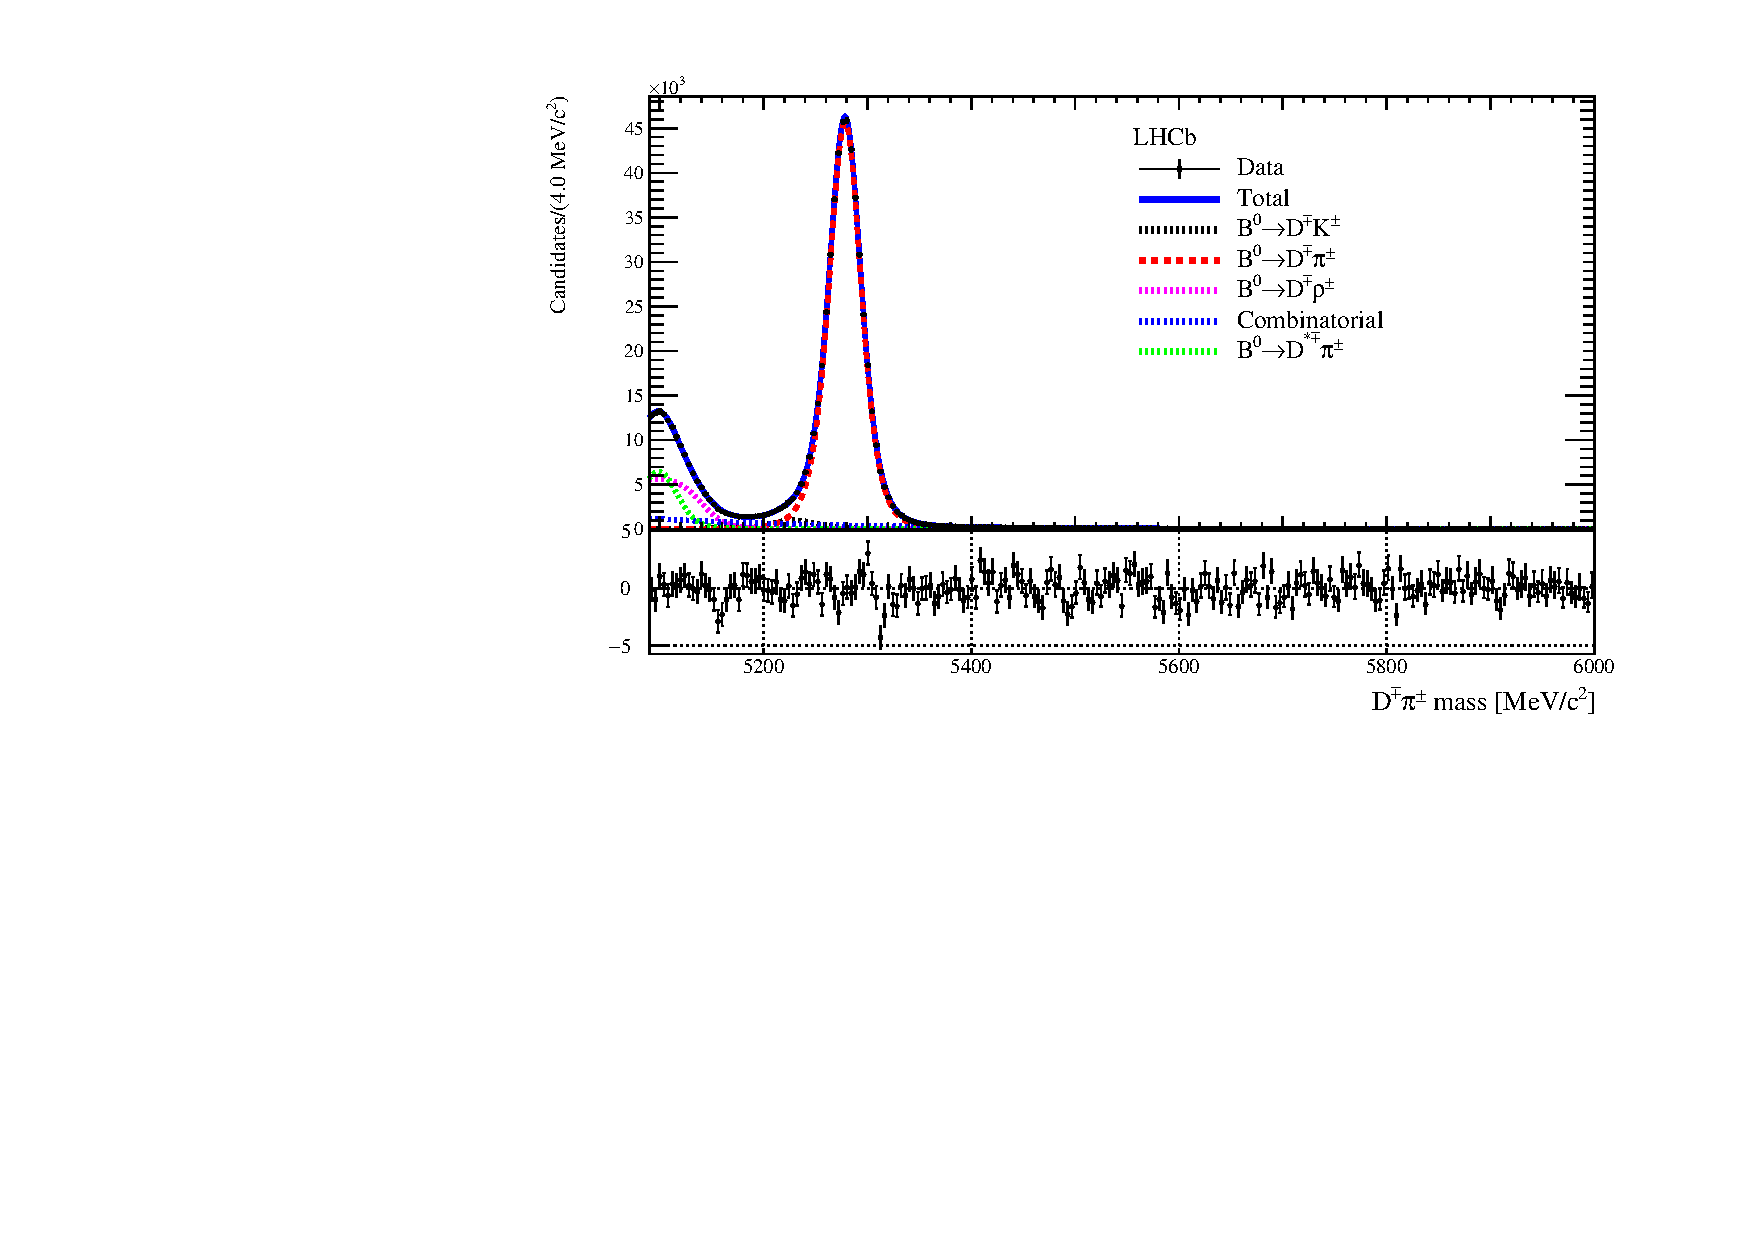
\includegraphics[width=\columnwidth]{03Massfit/figs/MDFitPlots_Bd/MDFit_BeautyMass_Bd2DPi_withPulls.pdf} \\
		\vspace{5mm}
                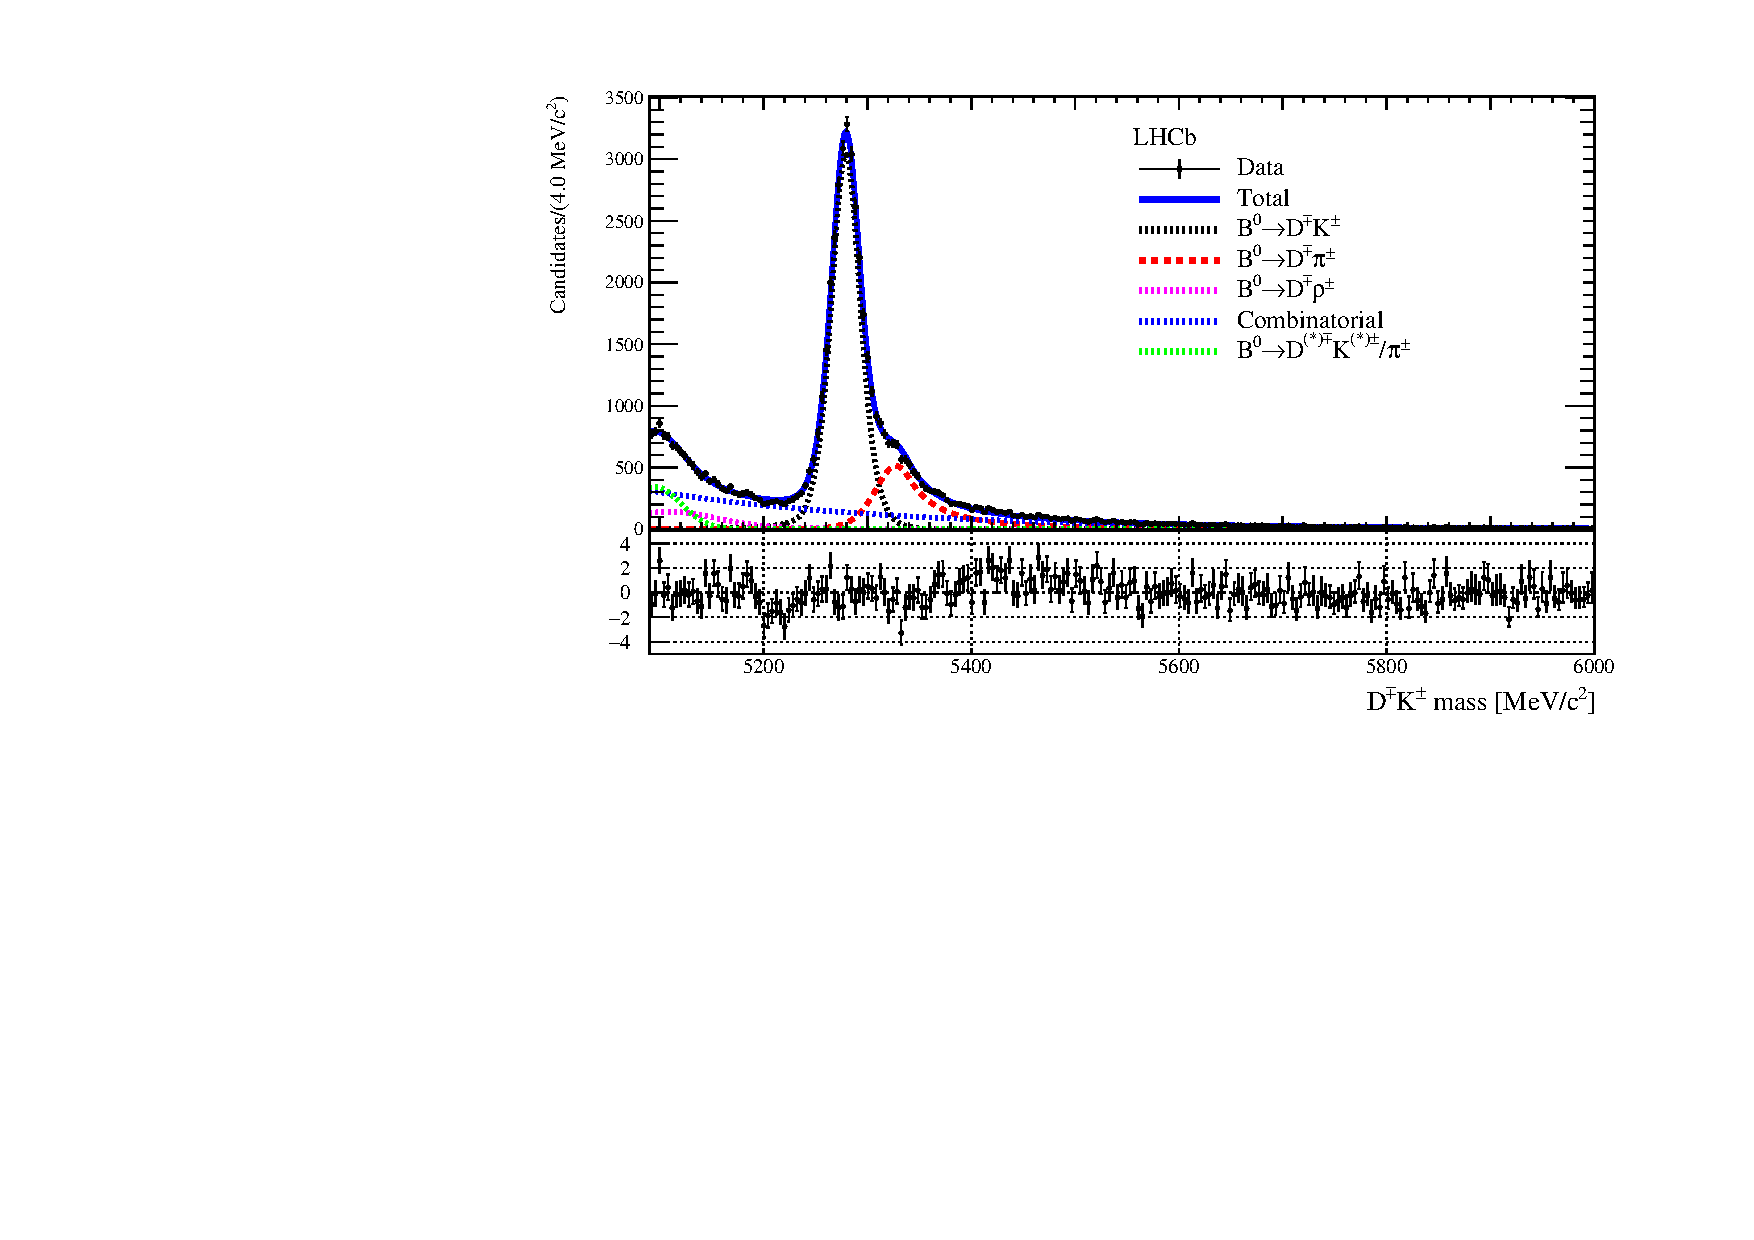
\includegraphics[width=\columnwidth]{03Massfit/figs/MDFitPlots_Bd/MDFit_BeautyMass_Bd2DK_withPulls.pdf}
	\end{center}
        \vspace{-2mm}
	\caption{Top: $\Dmp\pipm$ mass distribution of the $\pi$ sample. Bottom: $\Dmp\Kpm$ mass distribution of the $K$ sample. 
		     The result of the simultaneous fit (Fit A) to both samples is superimposed.
		     The plot below each histogram shows the normalised fit residuals (data minus fit divided by fit error).}
	\label{fig:FitA}
\end{figure}
\begin{table}
	\begin{center}
		\caption{Parameters of $f_{\pi}(m)$ fixed or constrained in Fit A. All non-zero values are obtained
		from the fits to MC samples described in Sec.~\ref{sec:pdf}.}
		\begin{tabular}{ccc}
			\toprule
			Parameter & Value & Status in Fit A\\
			\hline
			$a1^{\pi}_{\Bz\to D\pi}$ & $0.722\pm0.091$ & constrained \\
			$a2^{\pi}_{\Bz\to D\pi}$ & $0.96\pm0.12$ & constrained \\
			$n1^{\pi}_{\Bz\to D\pi}$ & $5.92\pm0.92$ & constrained \\
			$n2^{\pi}_{\Bz\to D\pi}$ & $5.83\pm0.38$ & constrained \\
	                $\beta^{\pi}_{\Bz\to D\pi}$ & $0.0$ & fixed\\
			$\lambda^{\pi}_{\Bz\to D\pi}$ & $-1.240\pm0.060$ & fixed\\
			$\zeta^{\pi}_{\Bz\to D\pi}$ & $0.0$ & fixed\\
                        $f^{\pi}_{\Bz\to D\pi}$ & $0.436\pm0.060$ & fixed\\ 
			\hline
			$\sigma^{\pi}_{\Bz\to DK}$ & $23.43\pm0.42~\rm MeV/c^{2}$ & fixed\\
			$a1^{\pi}_{\Bz\to DK}$ & $0.898\pm0.025$ & fixed\\
			$a2^{\pi}_{\Bz\to DK}$ & $1.092\pm0.033$ & fixed\\
			$n1^{\pi}_{\Bz\to DK}$ & $3.83\pm0.40$ & fixed\\
			$n2^{\pi}_{\Bz\to DK}$ & $22.0\pm7.6$ & fixed\\
			$\beta^{\pi}_{\Bz\to DK}$ & $0.0$ & fixed\\
			$\lambda^{\pi}_{\Bz\to DK}$ & $-24\pm10$ & fixed\\
			$\zeta^{\pi}_{\Bz\to DK}$ & $0.0$ & fixed\\
			\hline
			$\nu^{\pi}_{\Bz\to D\rho}$ & $-2.01\pm0.15$ & fixed\\
			$\mu^{\pi}_{\Bz\to D\rho}$ & $4\,828\pm80~\rm MeV/c^{2}$ & constrained into $\Delta\mu^{\pi}_{\Bz\to D\rho}$\\
			$\sigma^{\pi}_{\Bz\to D\rho}$ & $550\pm190~\rm MeV/c^{2}$ & fixed\\
			$\tau^{\pi}_{\Bz\to D\rho}$ & $1.163\pm0.090$ & fixed\\
			\hline
			$\alpha^{\pi}_{\Bz\to \Dst\pi}$ & $-1.443\pm0.031$ & fixed\\
			$n^{\pi}_{\Bz\to \Dst\pi}$ & $4.65\pm0.30$ & fixed\\
			$\mu^{\pi}_{\Bz\to \Dst\pi}$ & $5\,100.93\pm0.23~\rm MeV/c^{2}$ & constrained into $\Delta\mu^{\pi}_{\Bz\to \Dst\pi}$\\
			$\sigma G^{\pi}_{\Bz\to \Dst\pi}$ & $16.52\pm0.20~\rm MeV/c^{2}$ & fixed\\
			$\sigma CB^{\pi}_{\Bz\to \Dst\pi}$ & $25.84\pm0.48~\rm MeV/c^{2}$ & fixed\\
			$f^{\pi}_{\Bz\to \Dst\pi}$ & $0.302\pm0.011$ & fixed\\
			\bottomrule
		\end{tabular}
		\label{tab:FitAfixedPisample}
	\end{center}
\end{table}
\begin{table}
	\begin{center}
		\caption{Parameters of $f_{K}(m)$ fixed or constrained in Fit A. All non-zero values are obtained
		from the fits to MC samples described in Sec.~\ref{sec:pdf}.}
		\begin{tabular}{ccc}
			\toprule
			Parameter & Value & Status in Fit A\\
			\hline
			$\sigma^{K}_{\Bz\to D\pi}$ & $23.97\pm0.46~\rm MeV/c^{2}$ & fixed\\
			$a1^{K}_{\Bz\to D\pi}$ & $3.14\pm0.14$ & fixed\\
			$a2^{K}_{\Bz\to D\pi}$ & $0.569\pm0.039$ & fixed\\
			$n1^{K}_{\Bz\to D\pi}$ & $0.05\pm0.11$ & fixed\\
			$n2^{K}_{\Bz\to D\pi}$ & $2.81\pm0.12$ & fixed\\
			$\beta^{K}_{\Bz\to D\pi}$ & $0.0$ & fixed\\
			$\lambda^{K}_{\Bz\to D\pi}$ & $-3.77\pm0.57$ & fixed\\
			$\zeta^{K}_{\Bz\to D\pi}$ & $0.0$ & fixed\\
			\hline
			$\sigma^{K}_{\Bz\to DK}$ & $17.32\pm0.26~\rm MeV/c^{2}$ & fixed\\
			$a^{K}_{\Bz\to DK}$ & $2.34\pm0.19$ & fixed\\
			$n^{K}_{\Bz\to DK}$ & $1.56\pm0.33$ & fixed\\
			$\beta^{K}_{\Bz\to DK}$ & $0.0$ & fixed\\
			$\lambda^{K}_{\Bz\to DK}$ & $-3.45\pm0.34$ & fixed\\
			$\zeta^{K}_{\Bz\to DK}$ & $0.0$ & fixed\\
			\hline
			$f^{K}_{\Bz\to D\rho}$ & $0.58\pm0.17$ & fixed\\
			$\mu^{K}_{\Bz\to D\rho}$ & $5\,109\pm24~\rm MeV/c^{2}$ & constrained into $\Delta\mu^{K}_{\Bz\to D\rho}$\\
			$\sigma 1^{K}_{\Bz\to D\rho}$ & $117\pm18~\rm MeV/c^{2}$ & fixed\\
			$\sigma 2^{K}_{\Bz\to D\rho}$ & $45\pm16~\rm MeV/c^{2}$ & fixed\\
			\bottomrule
		\end{tabular}
		\label{tab:FitAfixedKsample}
	\end{center}
\end{table}
\begin{table}
	\begin{center}
		\caption{Results of Fit A.}
		\begin{tabular}{cc}
			\toprule
			Parameter & Fitted value \\
			\hline
                        $\mu^{\pi}_{\Bz\to DK}$ & $5\,228.62\pm0.92$ \\
                        $\sigma^{K}_{\Bz\to DK}$ & $17.17\pm0.15$  \\
                        $\mu^{K}_{\Bz\to D\Kst}$ & $5\,094.8\pm3.9$  \\
                        $\sigma^{K}_{\Bz\to D\Kst}$ & $25.5\pm2.6$ \\
                        $c1^{\pi}_{\rm comb}$ & $-0.00576\pm0.00017$  \\
                        $c2^{\pi}_{\rm comb}$ & $-0.0010\pm0.0010$  \\
                        $f^{\pi}_{\rm comb}$ & $0.899\pm0.025$  \\
                        $c^{K}_{\rm comb}$ & $-0.004397\pm0.000066$  \\
                        $\mu^{K}_{\Bz\to DK}$ & $5\,279.19\pm0.14$  \\
                        $\mu^{\pi}_{\Bz\to D\pi}$ & $5\,278.360\pm0.032$  \\
                        $sa^{\pi}_{\Bz\to D\pi}$ & $0.684\pm0.022$  \\
                        $sn^{\pi}_{\Bz\to D\pi}$ & $2.71\pm0.80$  \\
                        $\sigma H^{\pi}_{\Bz\to D\pi}$ & $37.69\pm0.69$ \\
                        $\sigma J^{\pi}_{\Bz\to D\pi}$ & $17.01\pm0.17$  \\
                        $\mu^{K}_{\Bz\to D\pi}$ & $5\,327.32\pm0.78$  \\
                        $\epsilon_{\rm PID}(\Bz\to DK)_{K}$ & $0.6197\pm0.0079$  \\
                        $\epsilon_{\rm PID}(\Bz\to D\pi)_{\pi}$ & $0.98048\pm0.00041$  \\
                        $N^{K}_{\Bz\to DK}$ & $28\,820\pm242$ \\
                        $N^{K}_{\Bz\to D\Kst}$ & $3\,164\pm110$ \\
                        $N^{\pi}_{\Bz\to D\rho}$ & $73\,766\pm1239$ \\
                        $N^{\pi}_{\Bz\to \Dst\pi}$ & $52\,494\pm819$ \\
                        $N^{K}_{\rm comb}$ & $17\,469\pm341$ \\
                        $N^{\pi}_{\rm comb}$ & $56\,230\pm1336$ \\
                        $N^{\pi}_{\Bz\to D\pi}$ & $483\,398\pm1040$ \\
			\bottomrule
		\end{tabular}
		\label{tab:FitAfloating}
	\end{center}
\end{table}

\iffalse
\begin{figure}[htbp]
	\begin{center}
		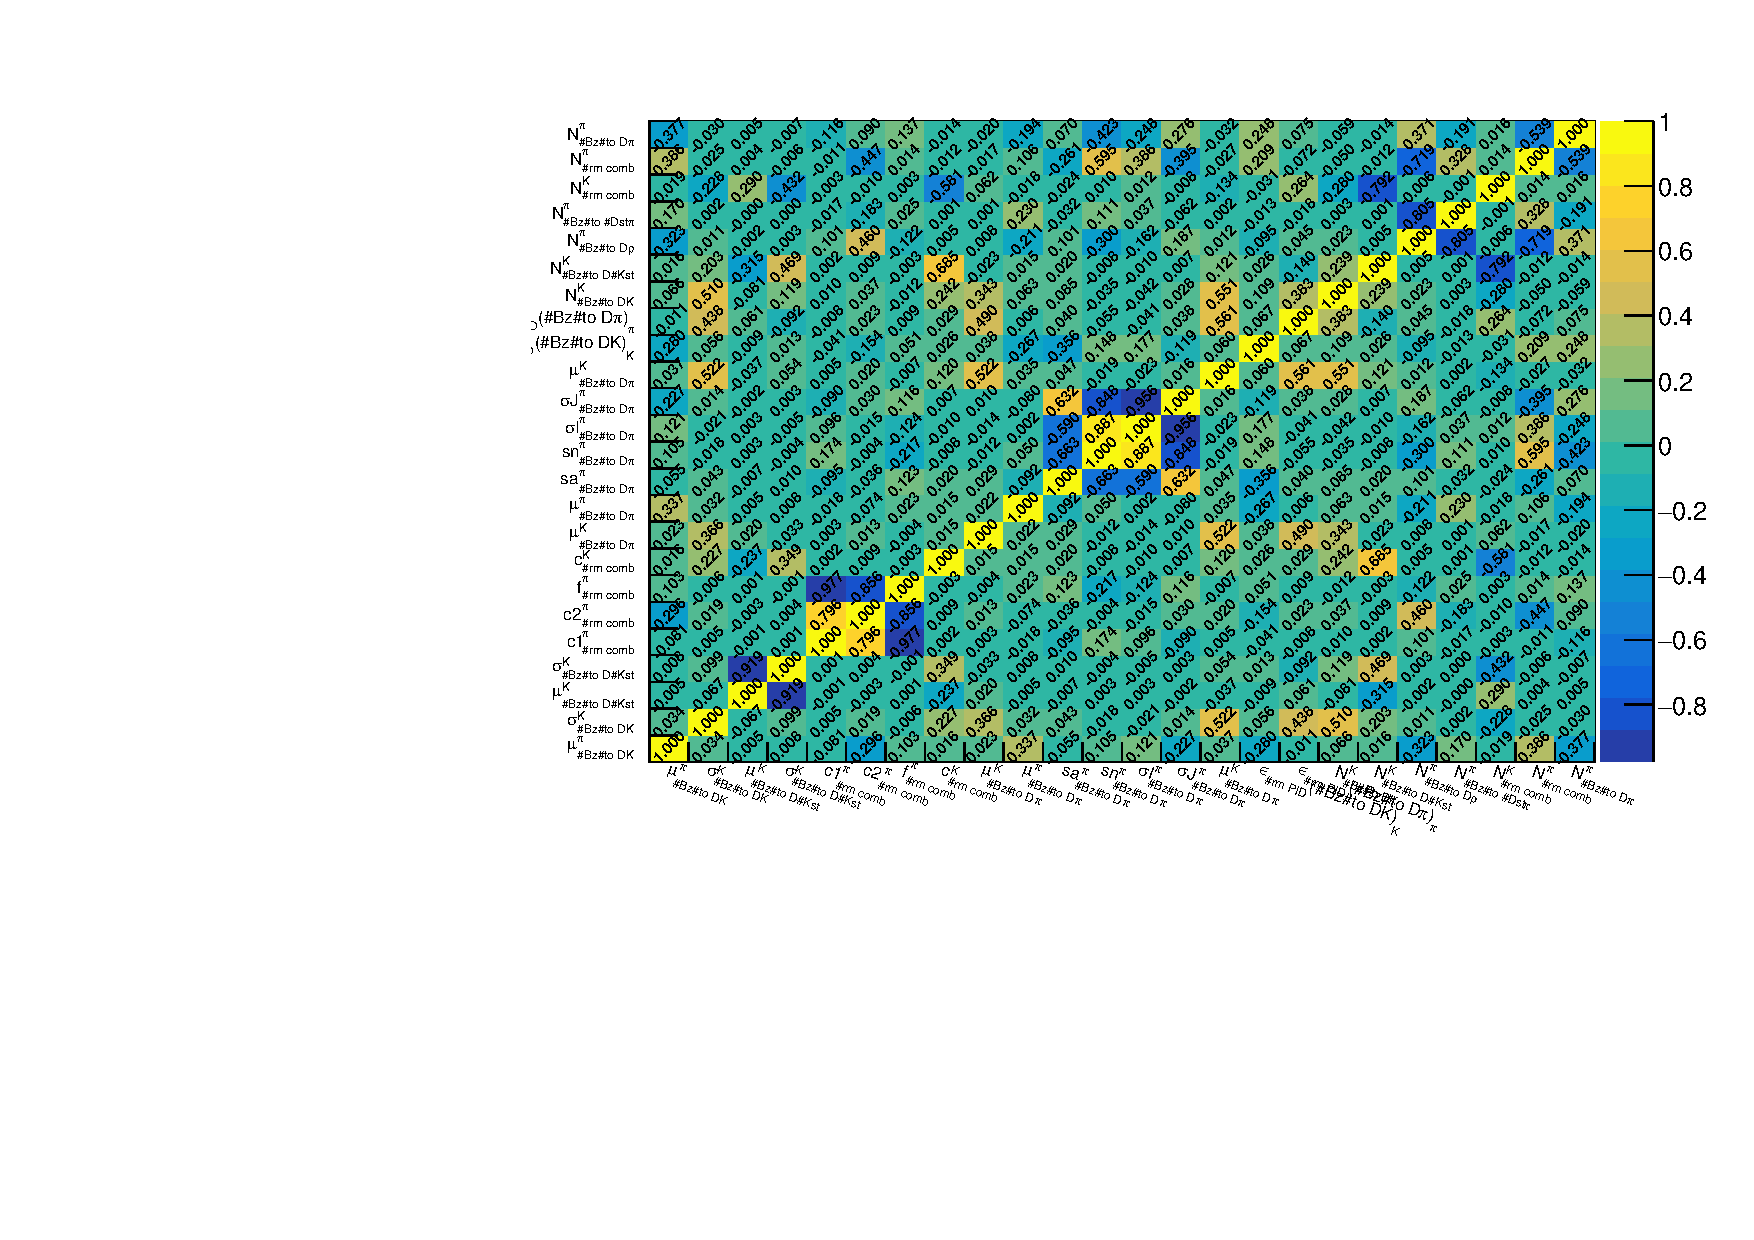
\includegraphics[width=0.7\linewidth]{03Massfit/figs/MDFitPlots_Bd/MDFit_CorrelationMatrix.pdf} \\
	\end{center}
        \vspace{-2mm}
	\caption{Correlation matrix among the floating parameters of $\PDF_{\pi}$ and
	$\PDF_{K}$ in Fit A. The parameter numbers are defined in
	Table~\ref{tab:FitAfloating}.}
	\label{fig:corrFitA}
\end{figure}
\fi

\begin{table}
	\centering
	\caption{Expected and fitted yields for the physical background components in the pion sample.}
	\label{tab:expVSfitYields}
	\begin{tabular}{lrr}
		\toprule
		Decay & Expected yield $[10^{4}]$ & Fitted yield $[10^{4}]$ \\
		\hline
		$\Bz\to\Dm\Kp$ & $1.26\pm0.15$ & $1.65\pm0.05$ \\
		$\Bz\to\Dmp\rho^\pm$ & $8.1\pm1.4$ & $7.38\pm0.12$ \\
		$\Bz\to D^{*\mp}\pipm$ & $5.6\pm0.4$ & $5.25\pm0.08$ \\
		\bottomrule
	\end{tabular}
\end{table}


\subsection{\emph{sWeight} calculation}
\label{sec:fitB}

After Fit A, all the floating shape parameters in $f_{\pi}(m)$ are
fixed, all the background components in the $\pi$ sample are combined into a
single PDF, and the $\Bz$ mass range is restricted to $[5220,5600]~\rm MeV/c^{2}$.
Concretely, $f_{\pi}(m)$ is redefined as
%
\begin{equation}
	f_{\pi}(m) = N^{\pi}_{\Bz\to D\pi}{\rm{PDF}}^{\pi}_{\Bz\to D\pi} + N^{\pi}_{\rm bkg}{\rm{PDF}}^{\pi}_{\rm bkg}.
\end{equation}
%
The $N^{\pi}_{\rm bkg}$ parameter describes the total number of
background events in the new range. The ${\rm{PDF}}^{\pi}_{\rm bkg}$ function is
defined as:
%
\begin{equation}
	\begin{split}
		\rm{PDF}^{\pi}_{\rm bkg} &= f^{\pi}_{\rm comb}{\rm{PDF}}^{\pi}_{\rm comb}
		+ f^{\pi}_{\Bz\to DK}{\rm{PDF}}^{\pi}_{\Bz\to DK} + f^{\pi}_{\Bz\to D\rho}{\rm{PDF}}^{\pi}_{\Bz\to D\rho} \\
		& + (1 - f^{\pi}_{\rm comb} - f^{\pi}_{\Bz\to DK} - f^{\pi}_{\Bz\to D\rho}){\rm{PDF}}^{\pi}_{\Bz\to \Dst\pi}.
	\end{split}
\end{equation}
%
For each background component in the $\pi$ sample, the fraction
$f^{\pi}_{j}$ is determined by the following expression:
%
\begin{equation}
	f^{\pi}_{j} = \frac{ N^{\pi}_{j}\int_{5220~\rm MeV/c^{2}}^{5600~\rm MeV/c^{2}} {\rm{PDF}}^{\pi}_{j} \,\deriv m }{\sum_{i} N^{\pi}_{i} \int_{5220~\rm MeV/c^{2}}^{5600~\rm MeV/c^{2}} {\rm{PDF}}^{\pi}_{i} \,\deriv m},
\end{equation}
%
where the indices $i$ and $j$ run over the combinatorial, $\Bz\to\Dm\Kp$ and $\Bz\to\Dmp\rho^\pm$ background components
in the $\pi$ sample, and $N^{\pi}_{j}$ is the number of events of component $j$ in the old mass range.

An unbinned extended maximum
likelihood fit (Fit B) is then performed to the $\pi$ sample only. The only floating
parameters are the yields $N^{\pi}_{\Bz\to D\pi}$ and $N^{\pi}_{\rm bkg}$. The
result of the fit is reported in Table~\ref{tab:FitBfloating}.
The yields of the signal component and the total background as obtained in Fit B are compatible
with the yields of the signal and the sum of the yields of each background as obtained in Fit A
after integrating the PDFs in the Fit B mass range.
\begin{table}
	\begin{center}
		\caption{Results of Fit B (second column) and 
			     yields calculated by integrating the PDFs fitted in Fit A in the mass range used for Fit B (third column).}
		\begin{tabular}{ccc}
			\toprule
			Parameter & Fitted value (Fit B) & Fitted value (Fit A)  \\
			\hline
			$N^{\pi}_{\Bz\to D\pi}$ & $479\,045\pm732$ & $483\,398\pm1040$ \\
			$N^{\pi}_{\rm bkg}$ & $34\,381\pm300$ & $34\,615\pm664$ \\
			\bottomrule
		\end{tabular}
		\label{tab:FitBfloating}
	\end{center}
\end{table}

Fit B is used as starting point to apply the \emph{sPlot} technique and extract
\emph{sWeights} used to subtract the total background component from the $\pi$
sample. The projection of the fitted $f_{\pi}(m)$ in Fit B and a comparison
between the weighted and unweighted datasets projected over the $\Bz$ decay time
and $\Dmp$ invariant mass observables are reported in Fig.~\ref{fig:sWeightComp}.
%The distribution of \emph{sWeights} is shown in Fig.~\ref{fig:sWeightdistribution}.
\begin{figure}[t]
	\begin{center}
		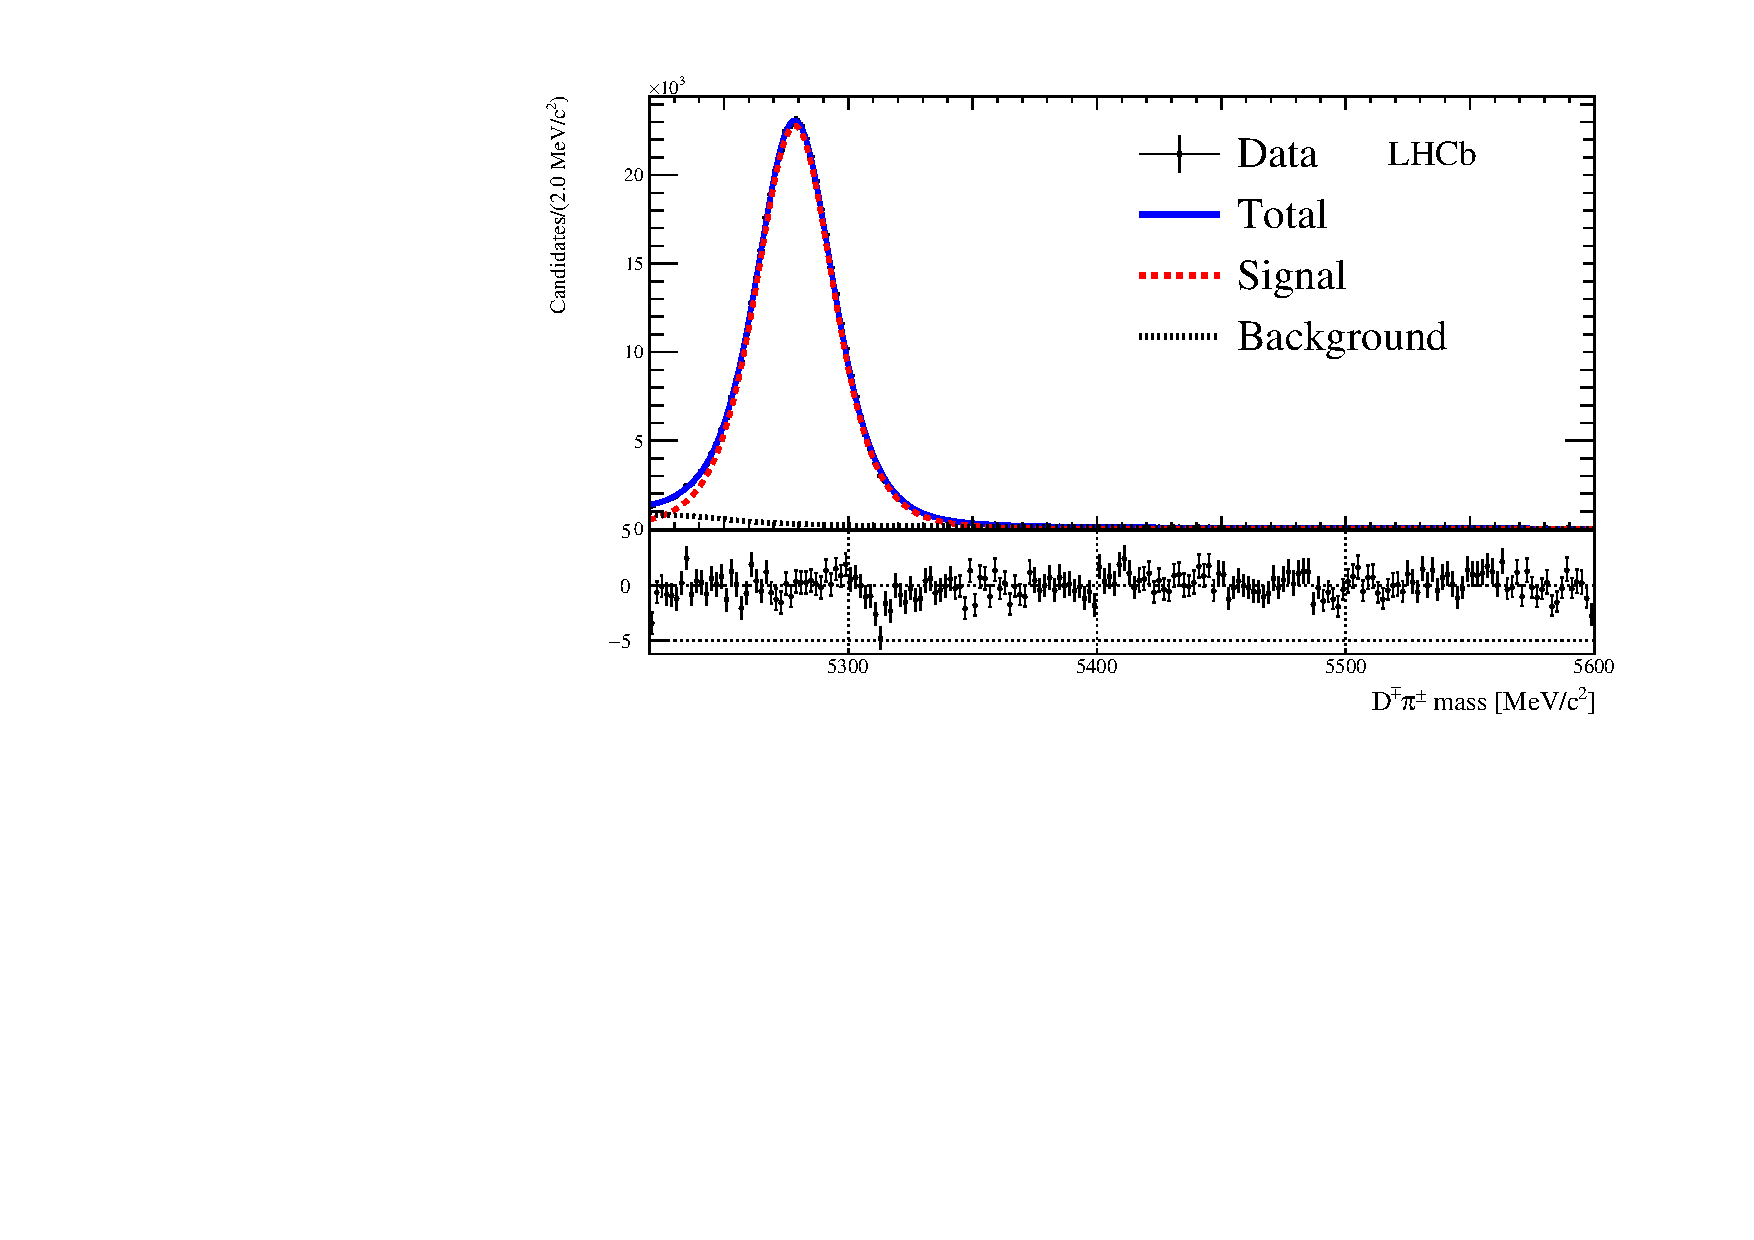
\includegraphics[width=0.65\linewidth]{03Massfit/figs/MDFitPlots_Bd/MDFitForSWeights_BeautyMass_Bd2DPi.pdf} \\
		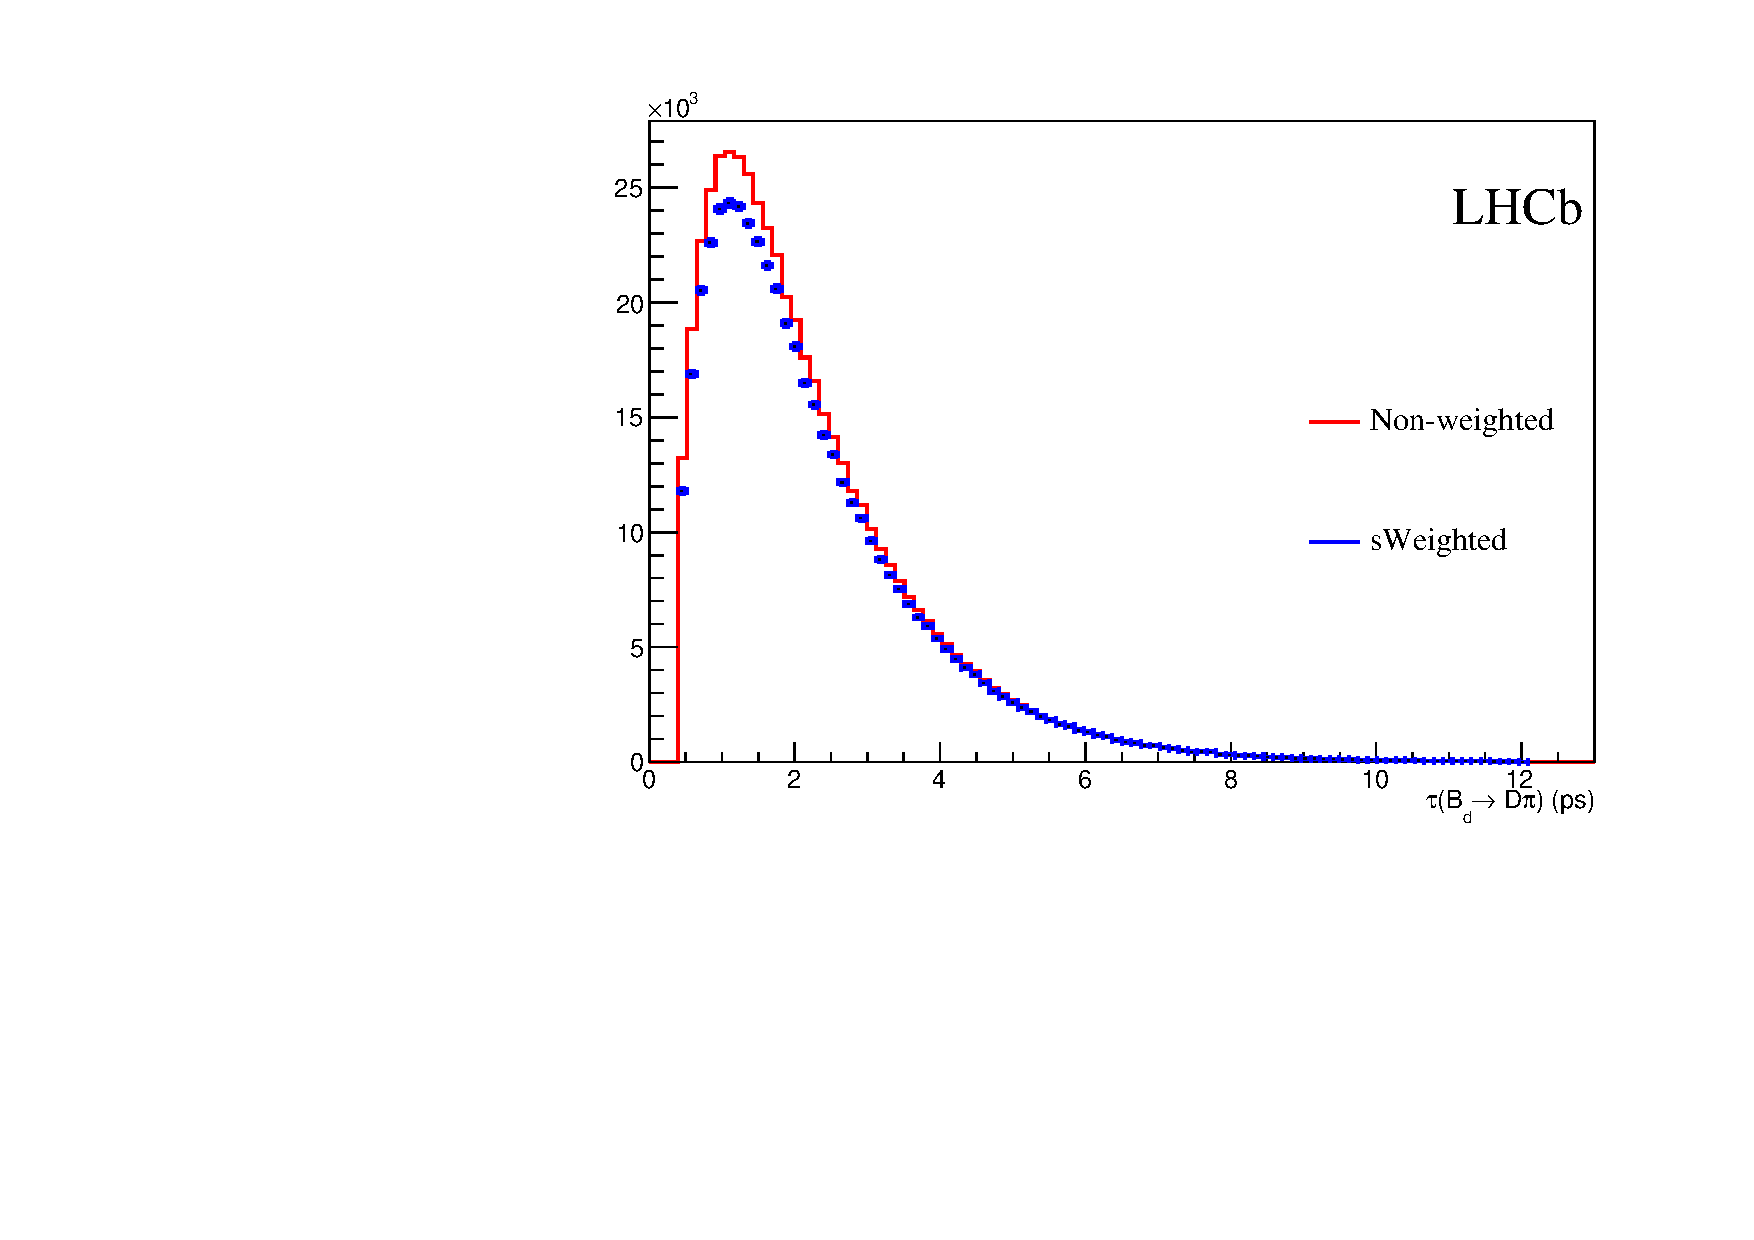
\includegraphics[width=0.45\linewidth]{03Massfit/figs/MDFitPlots_Bd/sWeightedDistribution_BeautyTime.pdf}
		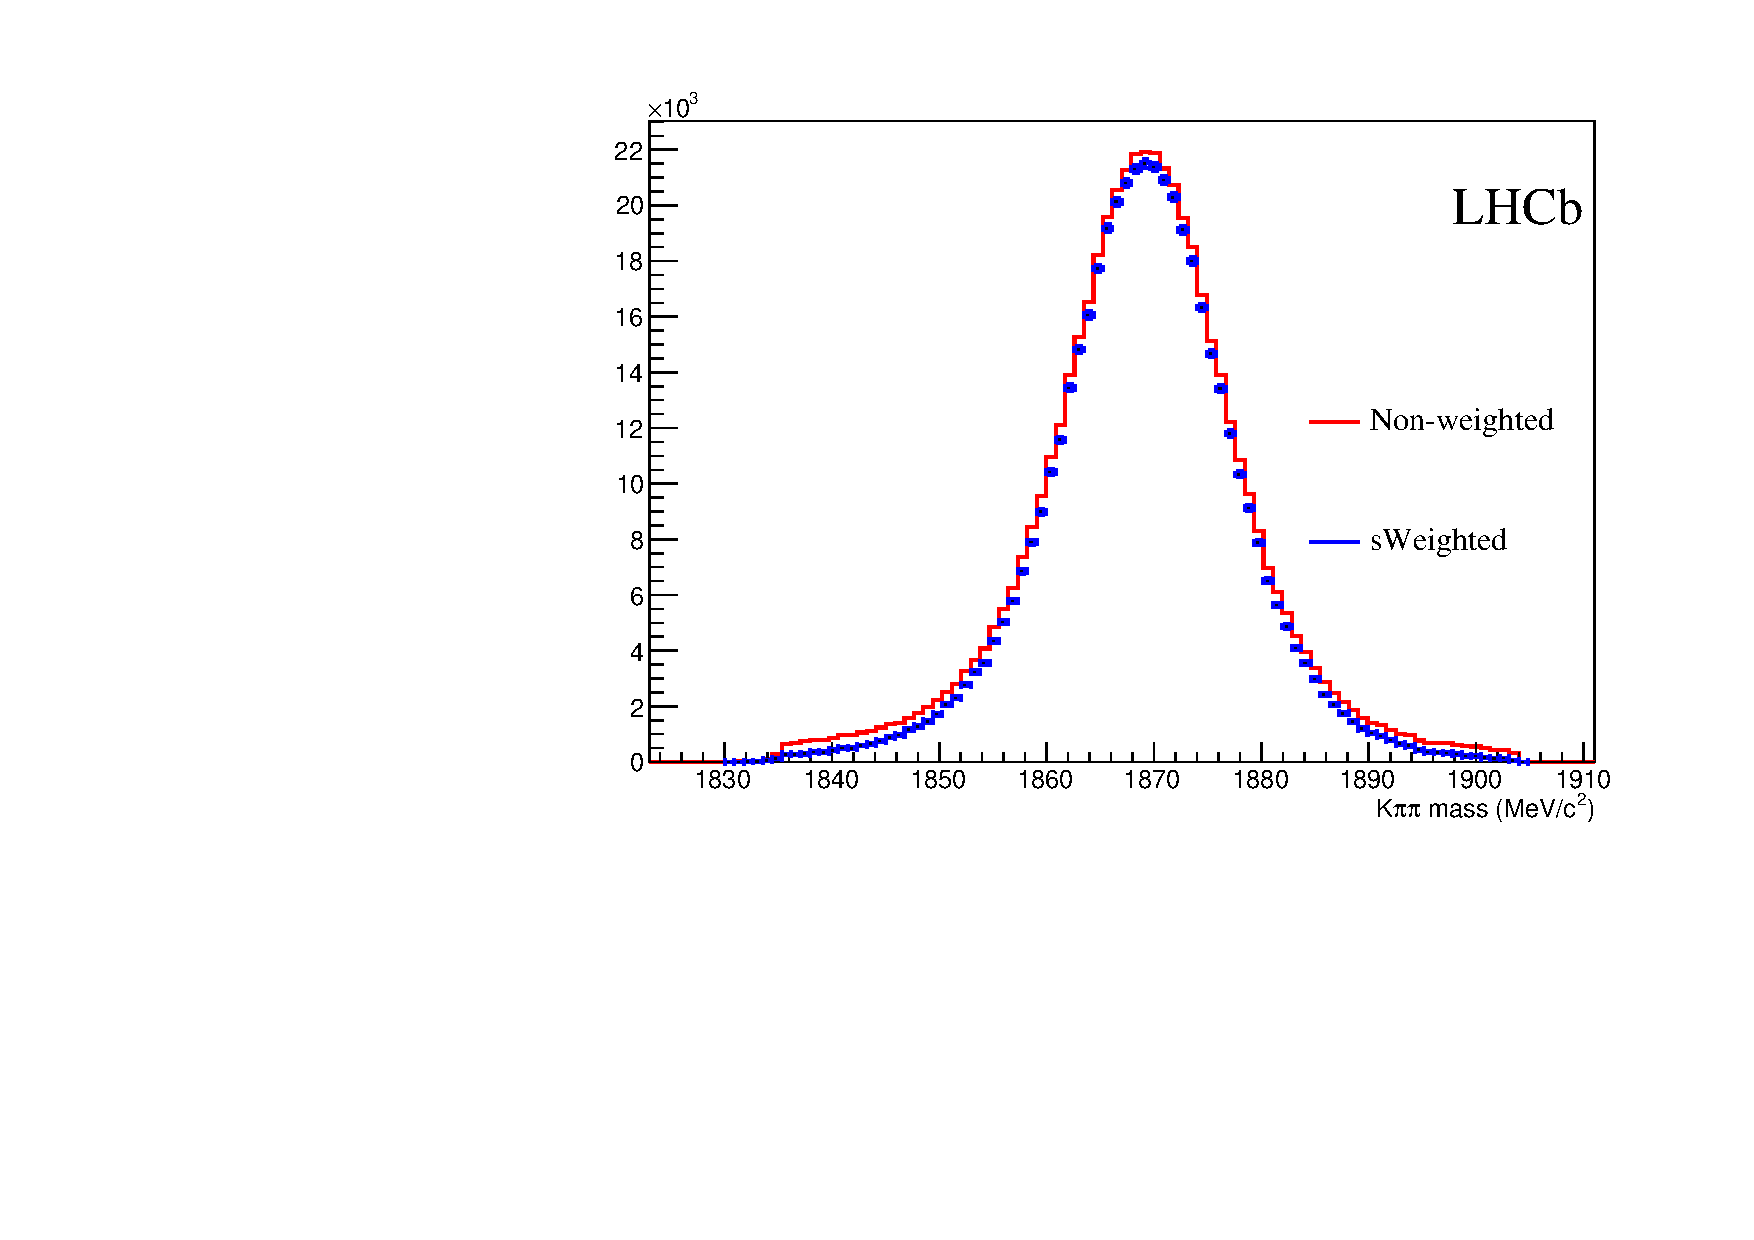
\includegraphics[width=0.45\linewidth]{03Massfit/figs/MDFitPlots_Bd/sWeightedDistribution_CharmMass.pdf}
	\end{center}
        \vspace{-2mm}
	\caption{Top: $\Dmp\pipm$ mass distribution of the $\pi$ sample with the results of Fit B superimposed. 
	The plot below the histogram shows the normalised fit residuals (data minus fit divided by fit error). Bottom: $\Bz$ decay time (left) and $\Kmp\pipm\pipm$ mass (right) distributions of the $\pi$
	sample in the $\Bz$ mass region $[5220,5600]~\mevcc$, with (blue) and without (red) \emph{sWeights} from Fit B.}
	\label{fig:sWeightComp}
\end{figure}

\iffalse
\begin{figure}[t]
	\begin{center}
		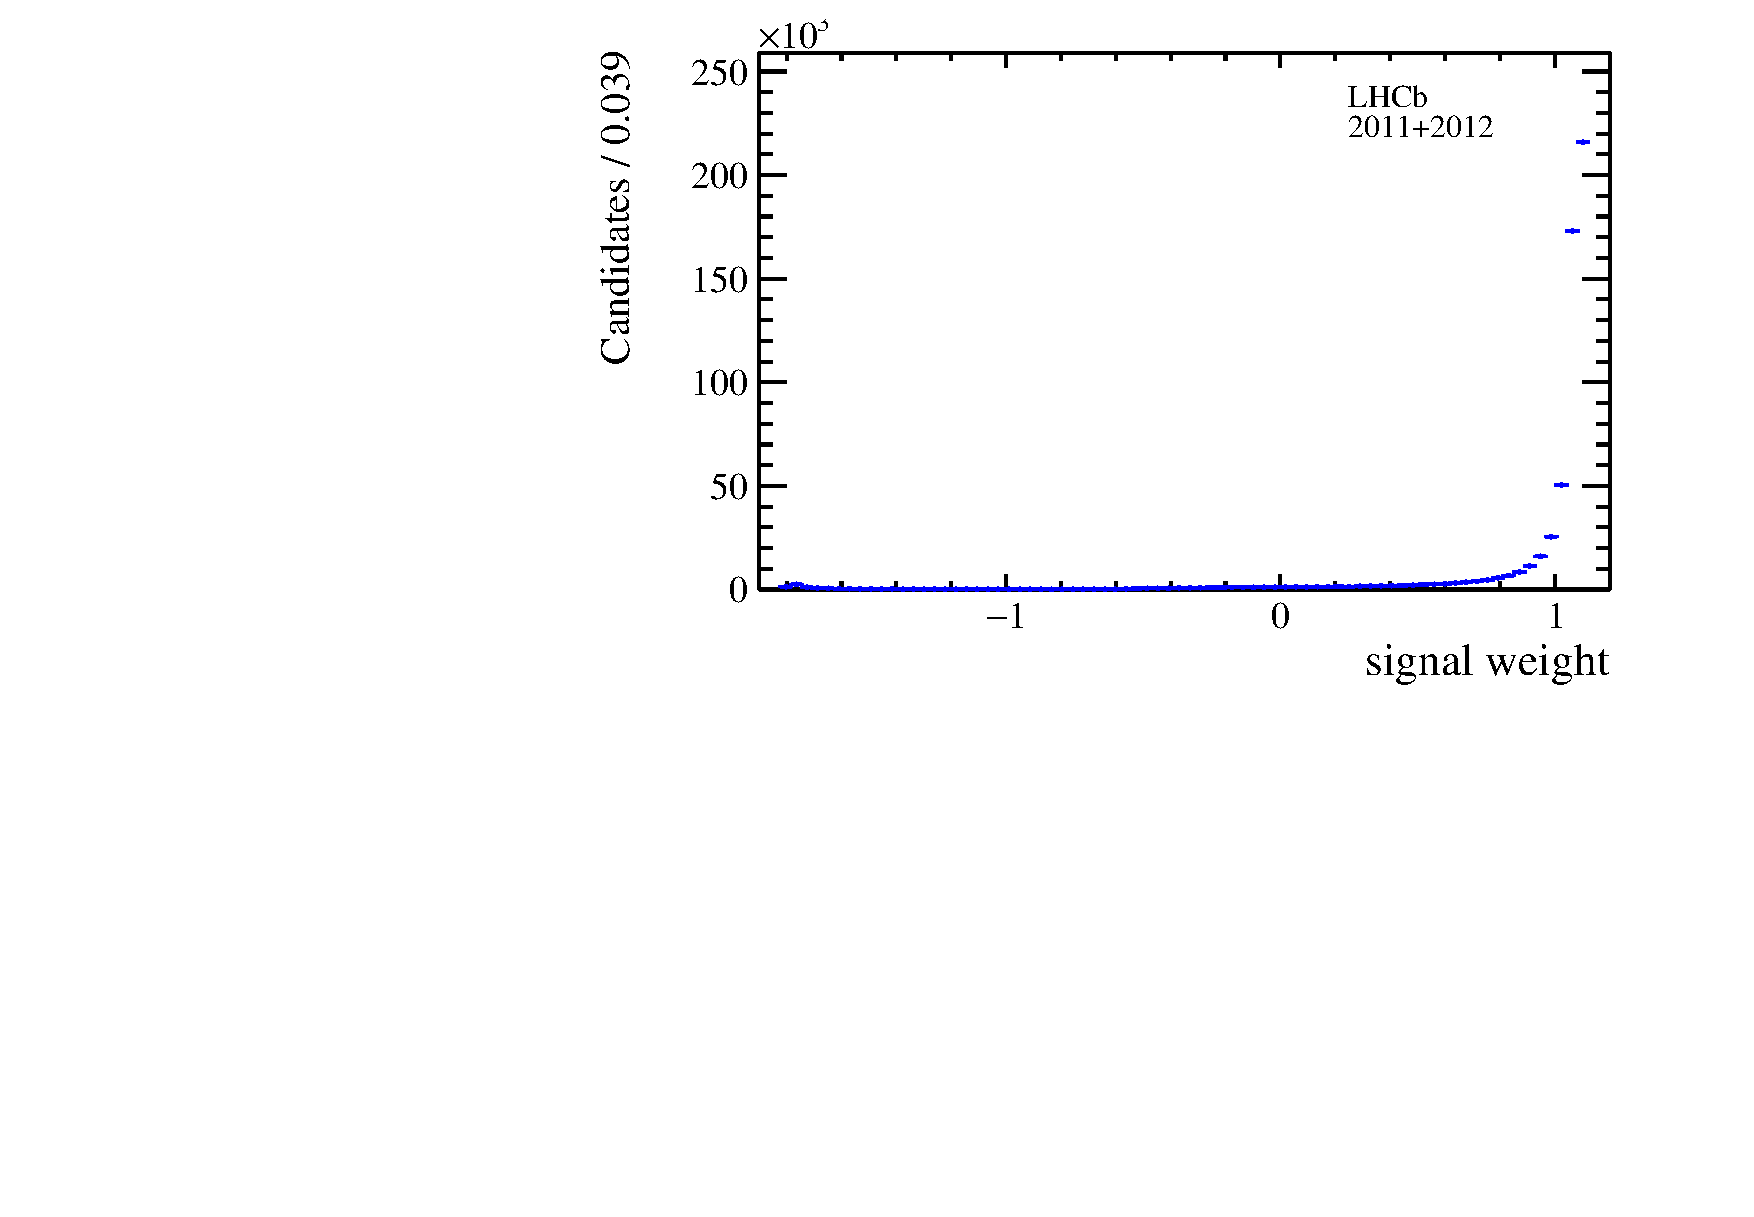
\includegraphics[width=0.65\linewidth]{03Massfit/figs/sweight_distribution.pdf}
	\end{center}
        \vspace{-2mm}
	\caption{Distribution of \emph{sWeights} obtained from Fit B.}
	\label{fig:sWeightdistribution}
\end{figure}
\fi

%-------------------------------------------------------------------------------
\subsection{Fits of subsamples}
\label{sec:split}
In order to validate the data sample, selection and fit procedure,
Fit A is repeated in smaller subsamples. These subsamples are divided per year of data taking
(2011, 2012), magnet polarity (up, down) and final state ($\Dp\pim$, $\Dm\pip$).
In order to cope with the reduced statistics in the 2011 subsample, the combinatorial background PDF of the $K$ sample (${\rm{PDF}}^{K}_{\rm comb}$ is taken as a simple exponential (instead of an exponential plus a constant function).
The projections of the fitted PDFs describing the pion and kaon samples for each data
subsample are shown in Figs.~\ref{fig:splitfitPi}
and~\ref{fig:splitfitK}, respectively.
\begin{figure}[t]
	\begin{center}
		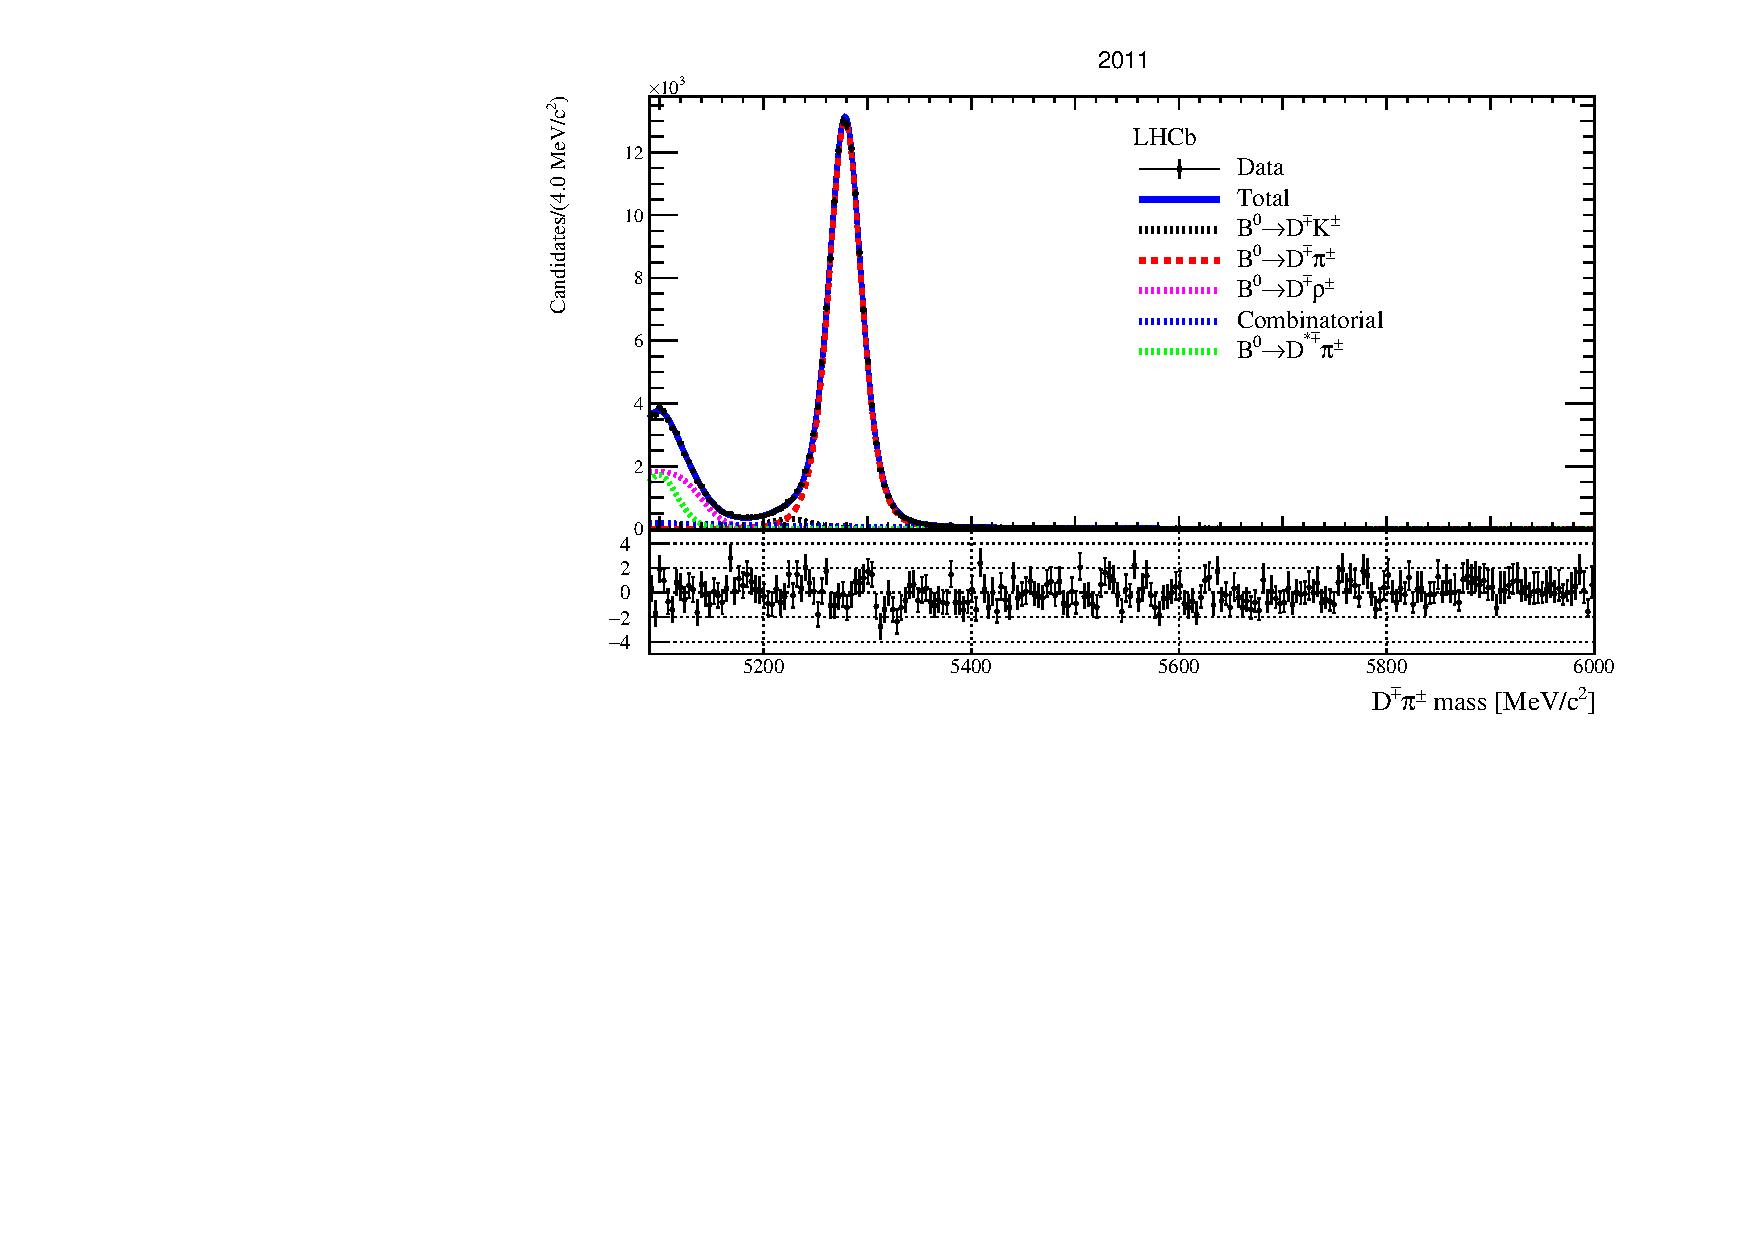
\includegraphics[width=0.48\linewidth]{03Massfit/figs/MDFitPlots_Bd_2011/MDFit_BeautyMass_Bd2DPi_withPulls.pdf}
		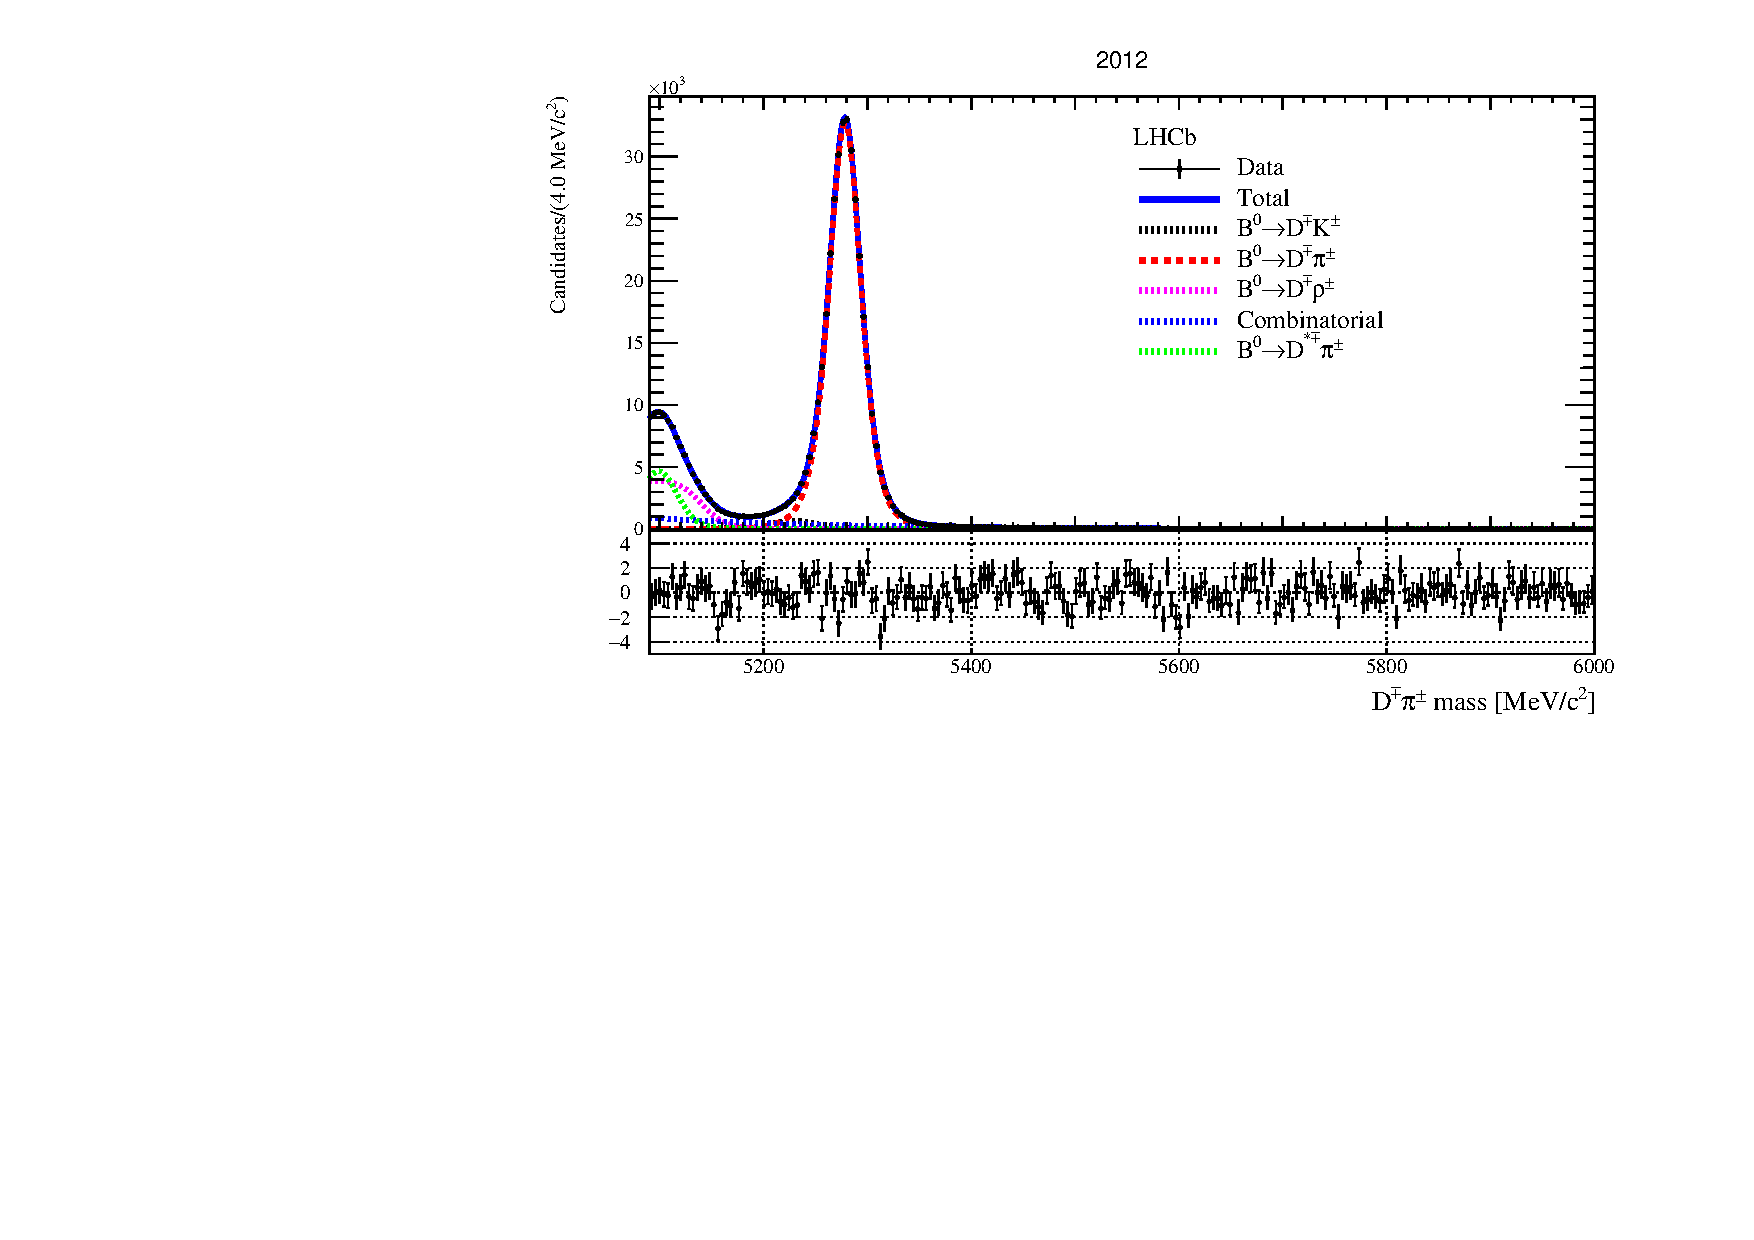
\includegraphics[width=0.48\linewidth]{03Massfit/figs/MDFitPlots_Bd_2012/MDFit_BeautyMass_Bd2DPi_withPulls.pdf} \\
		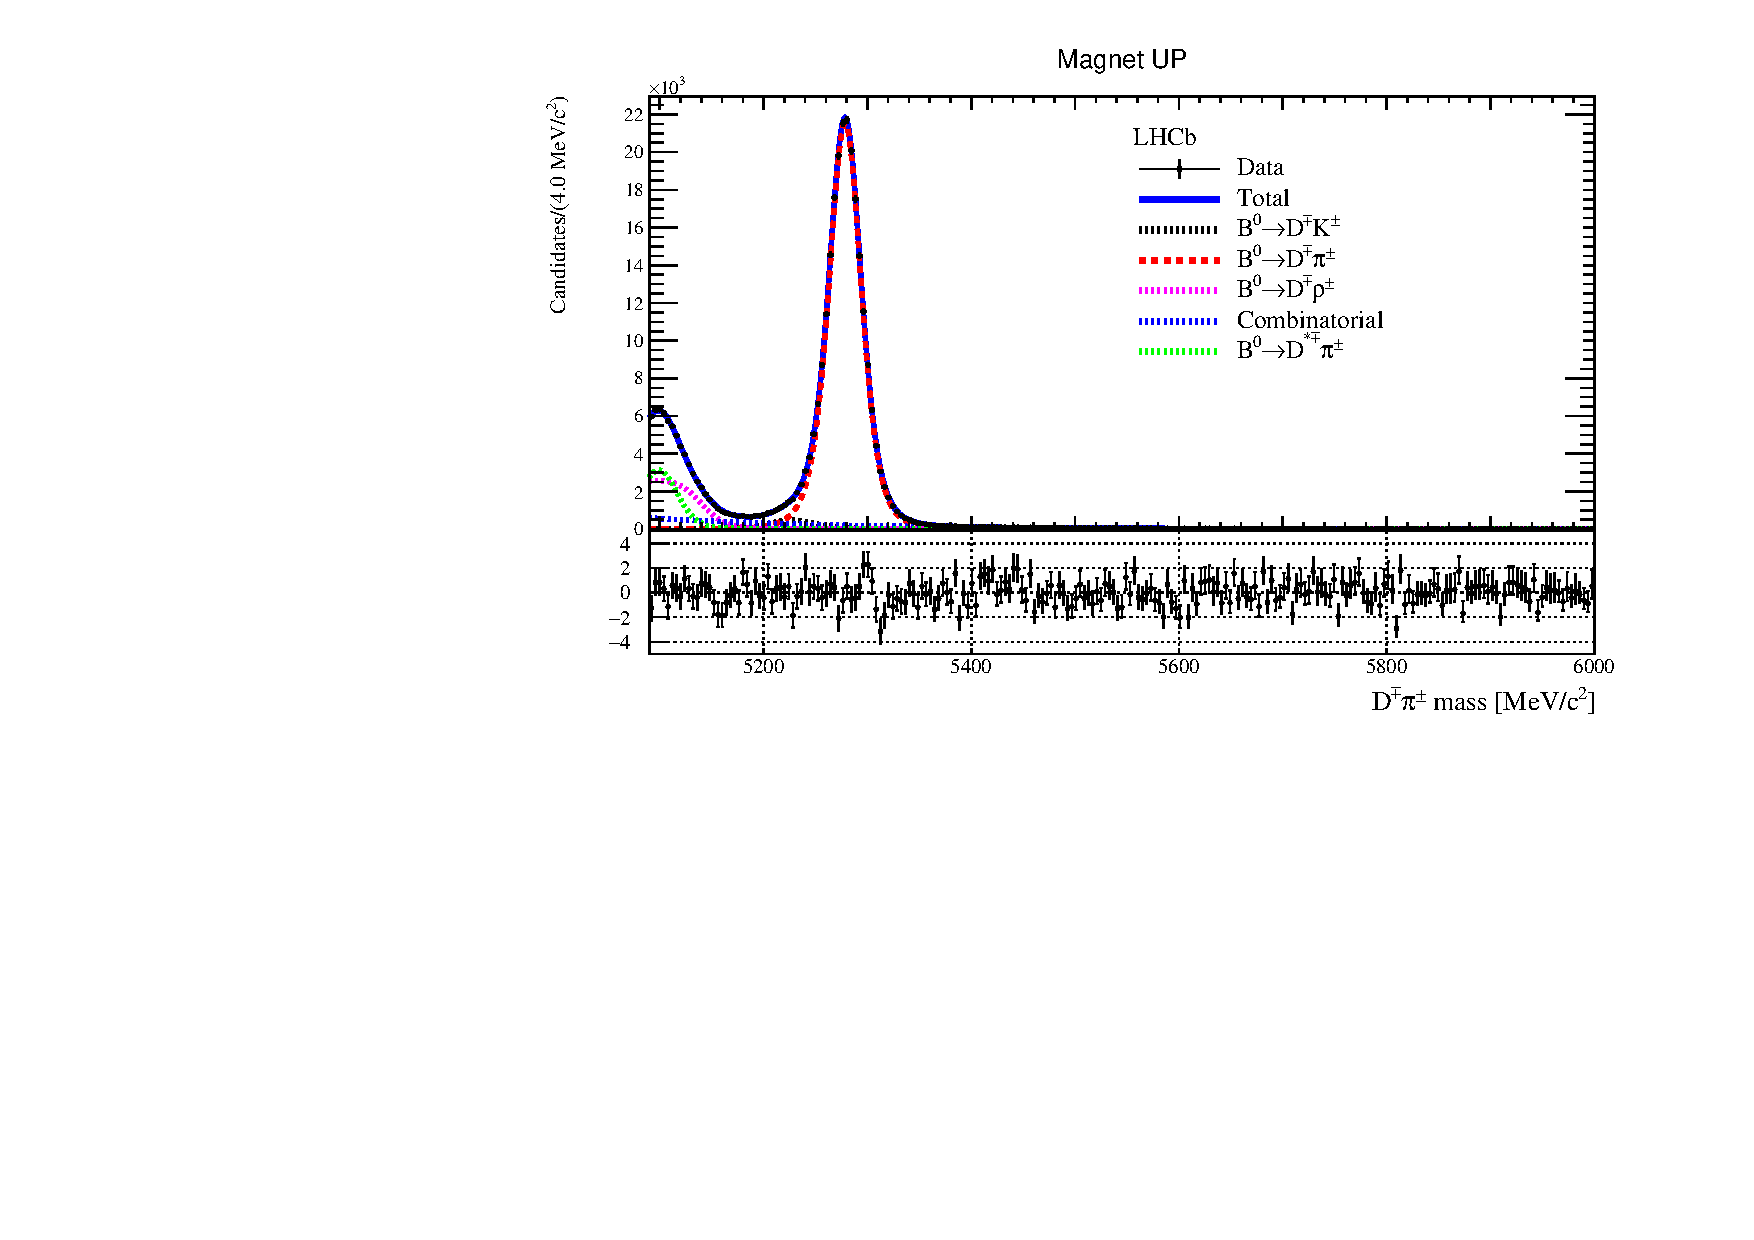
\includegraphics[width=0.48\linewidth]{03Massfit/figs/MDFitPlots_Bd_MU/MDFit_BeautyMass_Bd2DPi_withPulls.pdf}
		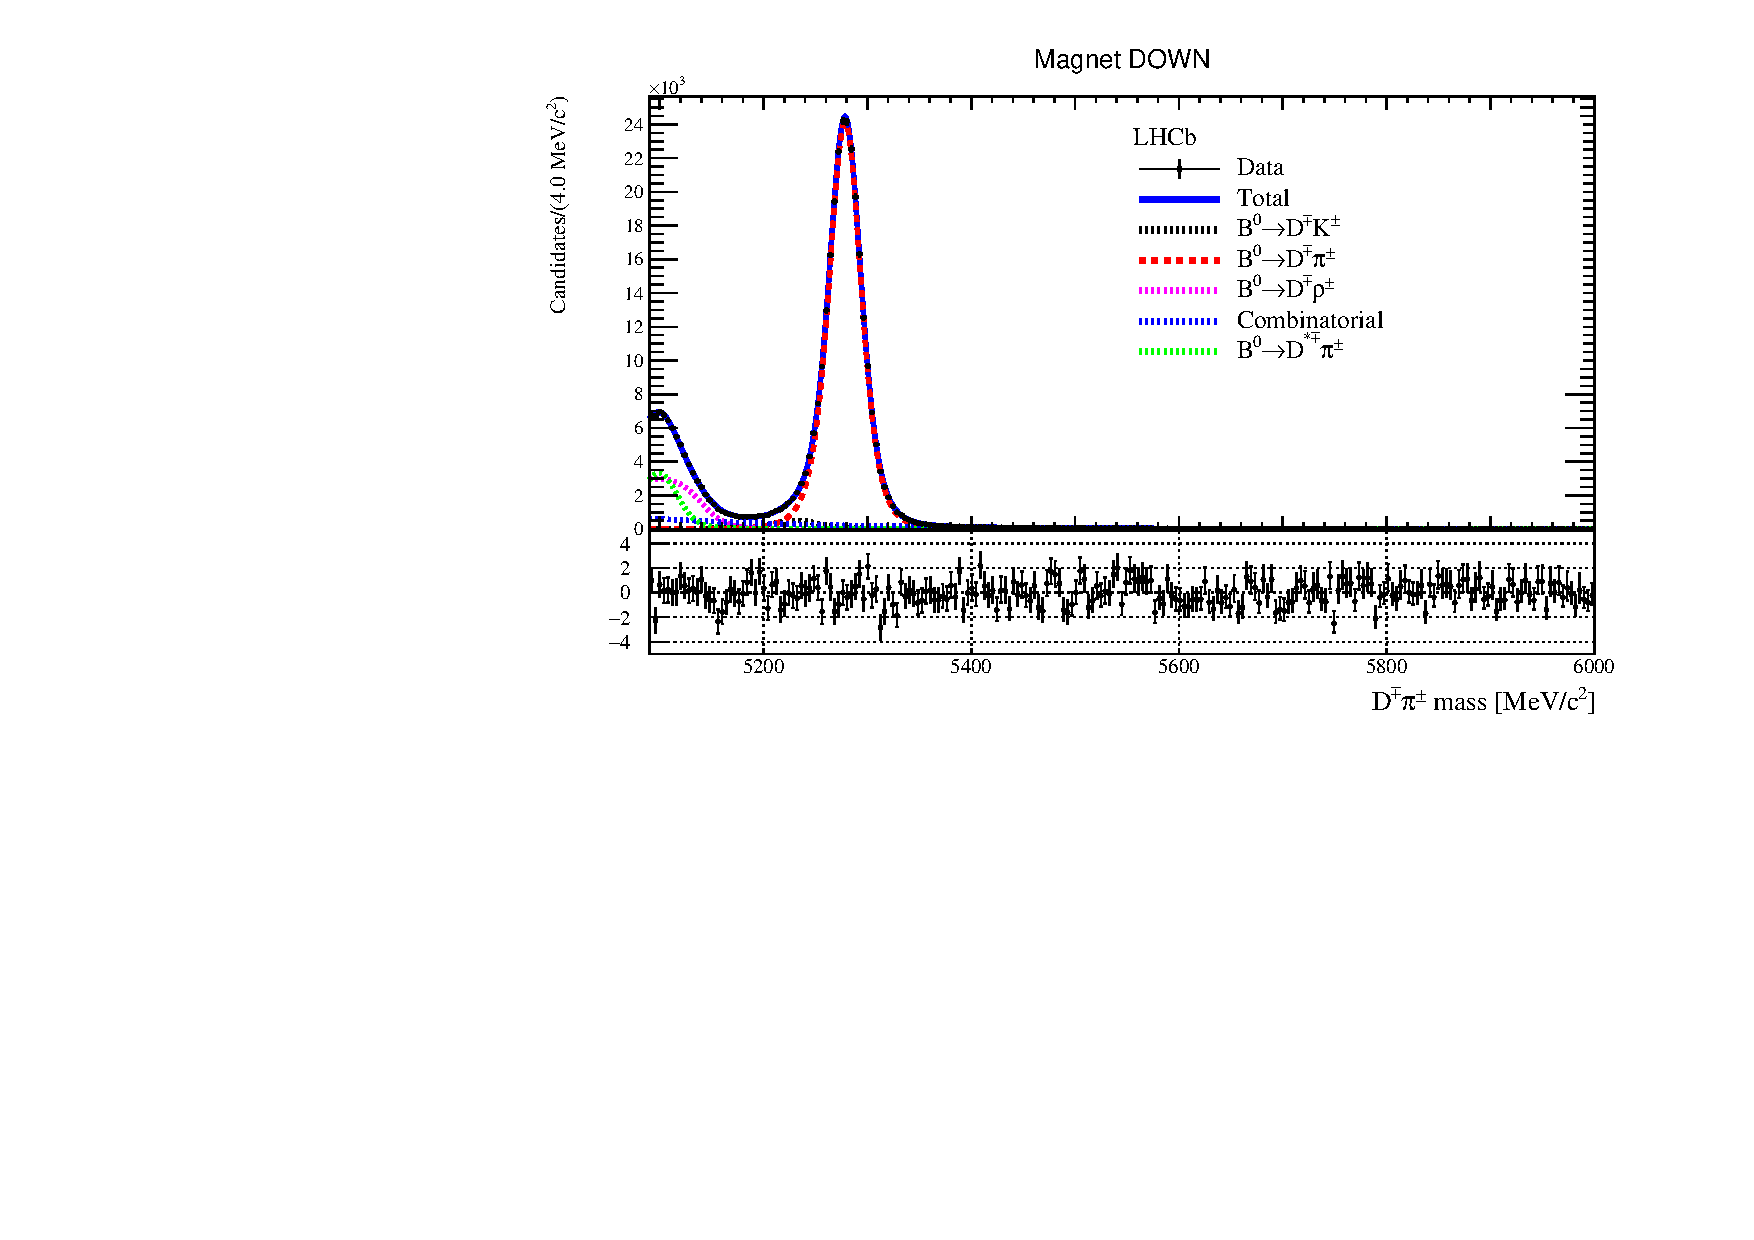
\includegraphics[width=0.48\linewidth]{03Massfit/figs/MDFitPlots_Bd_MD/MDFit_BeautyMass_Bd2DPi_withPulls.pdf} \\
		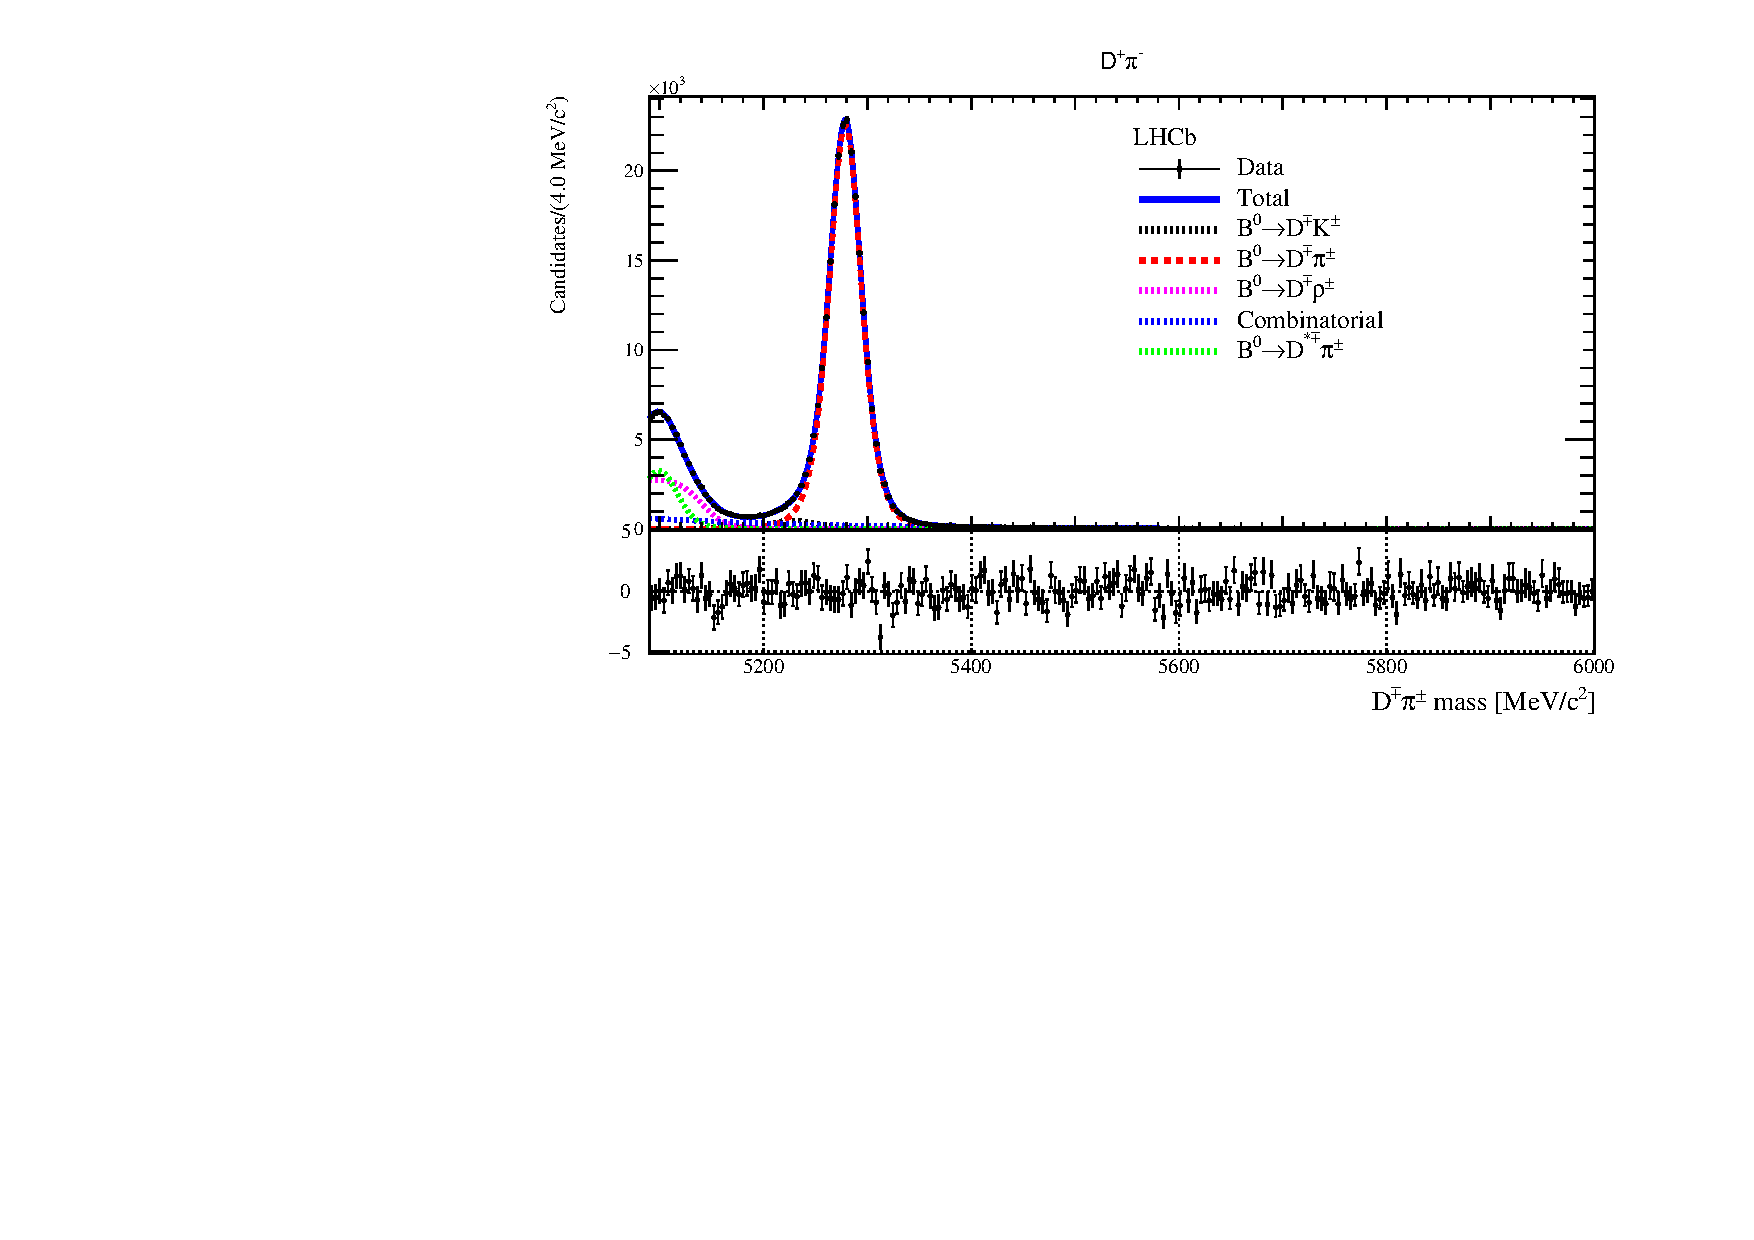
\includegraphics[width=0.48\linewidth]{03Massfit/figs/MDFitPlots_Bd_pim/MDFit_BeautyMass_Bd2DPi_withPulls.pdf}
		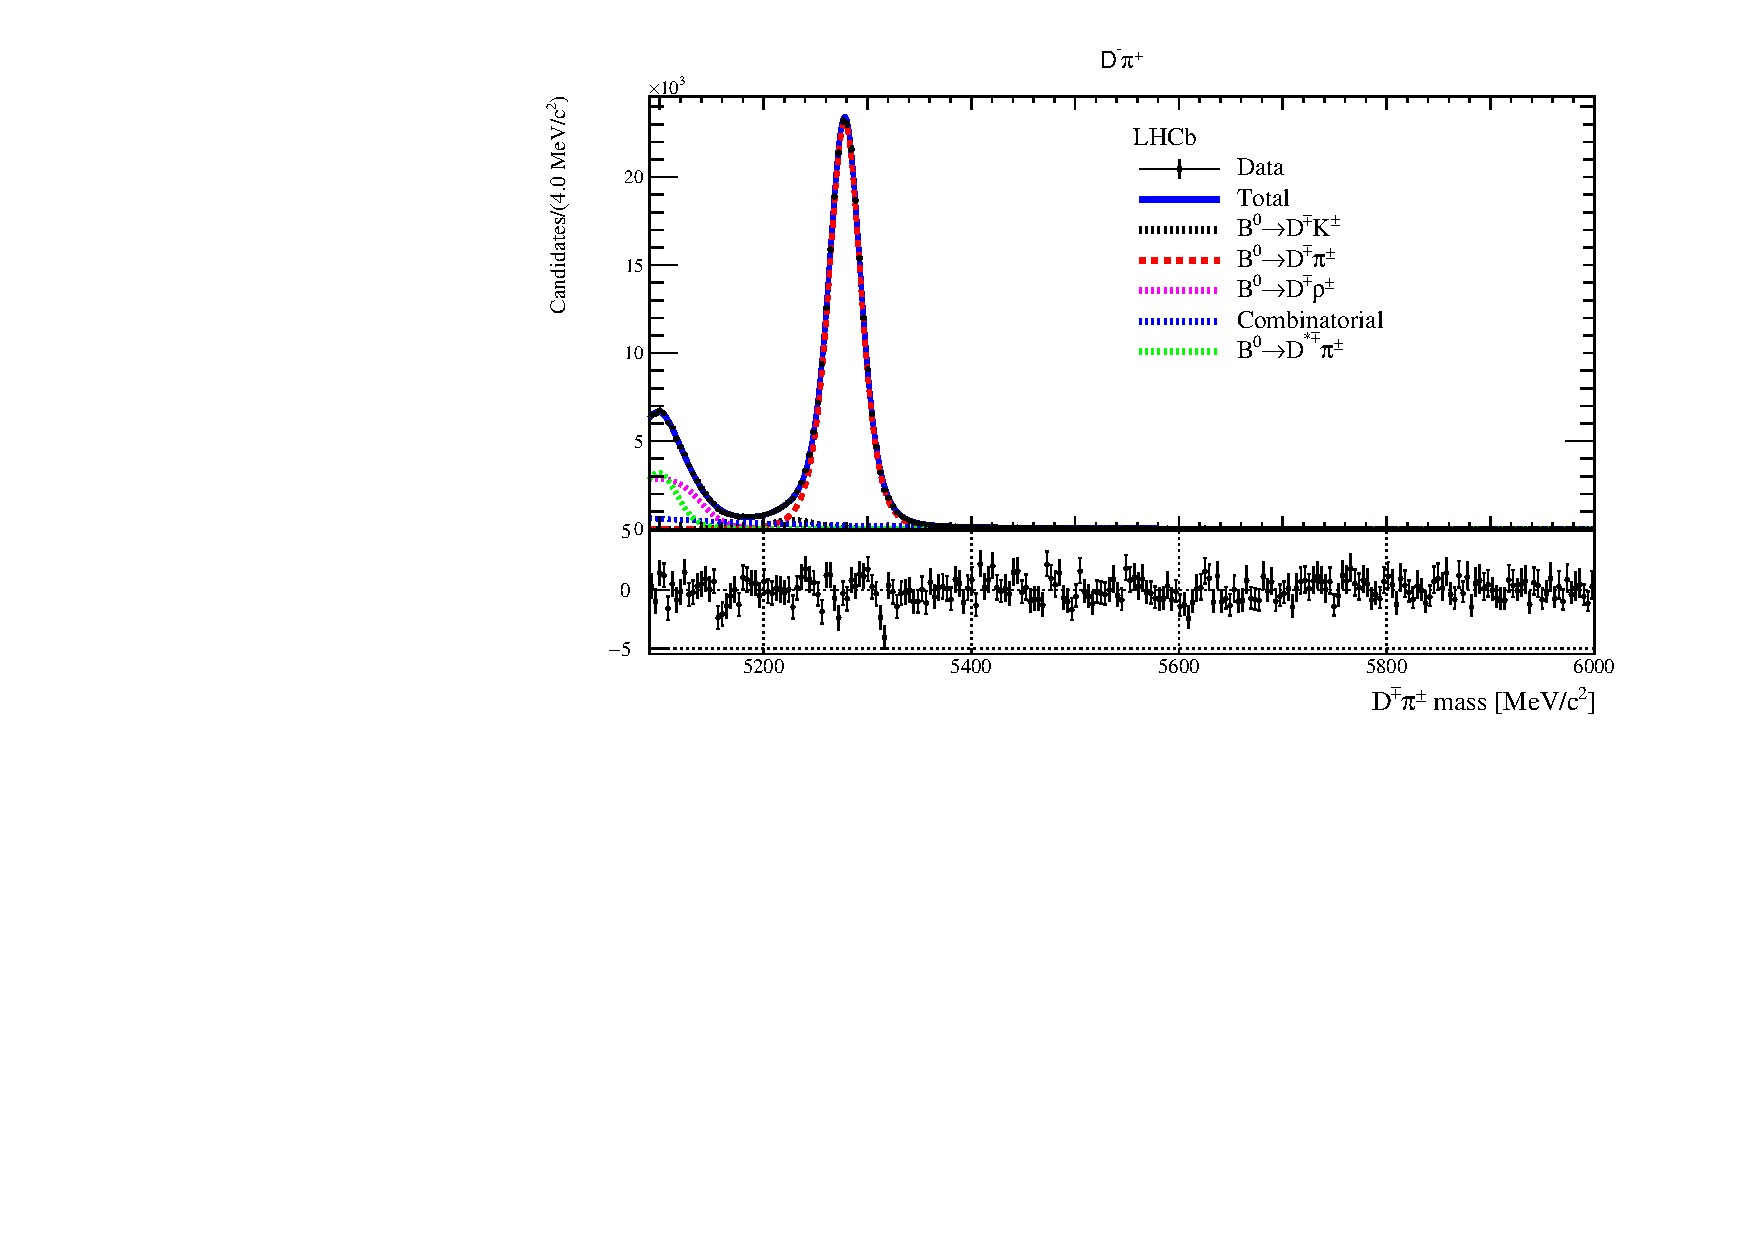
\includegraphics[width=0.48\linewidth]{03Massfit/figs/MDFitPlots_Bd_pip/MDFit_BeautyMass_Bd2DPi_withPulls.pdf} \\
		\vspace{-2mm}
                \caption{$\Dmp\pipm$ mass distributions of the pion sample for each data subsample, with the result of Fit A 
                  superimposed. The plots below the histograms show the normalised fit residuals.
		\label{fig:splitfitPi}}
	\end{center}
\end{figure}
\begin{figure}[htbp]
	\begin{center}
		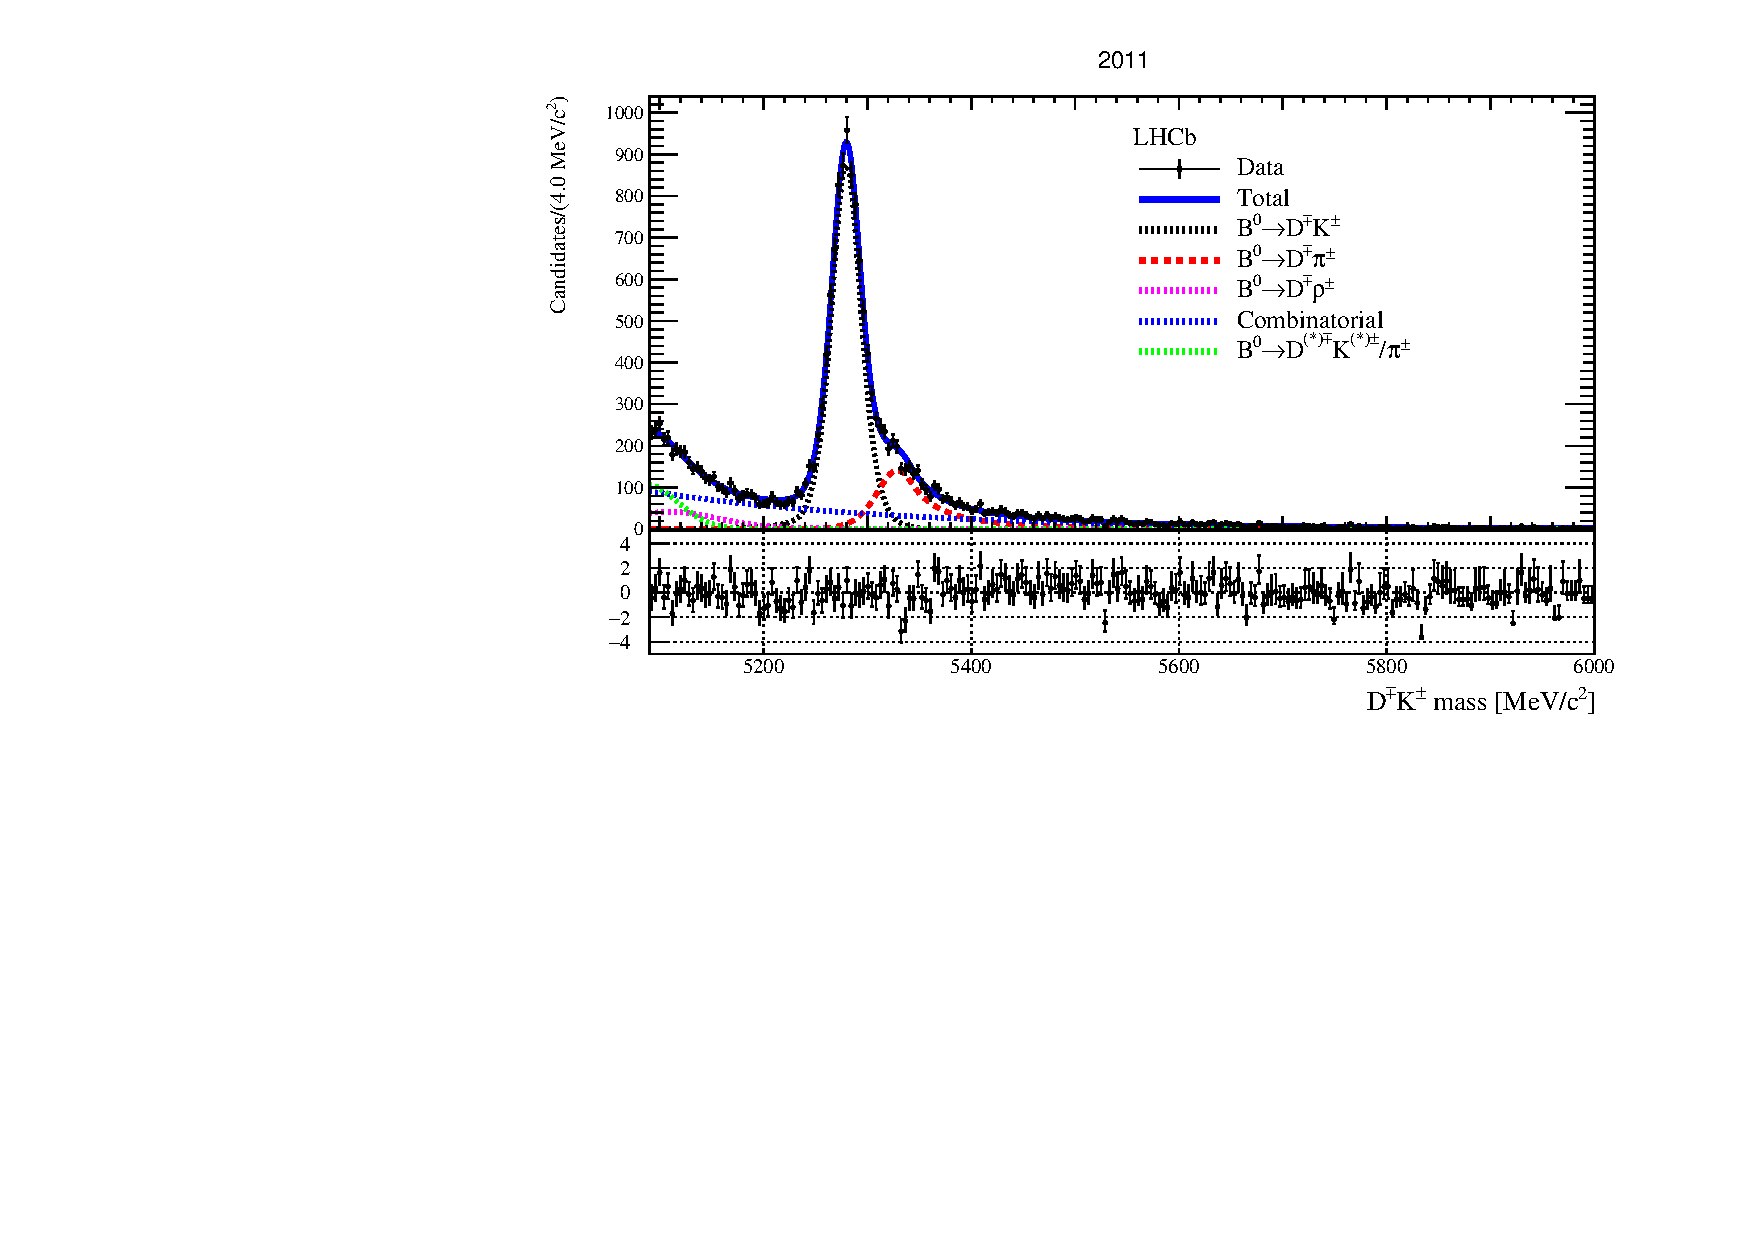
\includegraphics[width=0.48\linewidth]{03Massfit/figs/MDFitPlots_Bd_2011/MDFit_BeautyMass_Bd2DK_withPulls.pdf}
		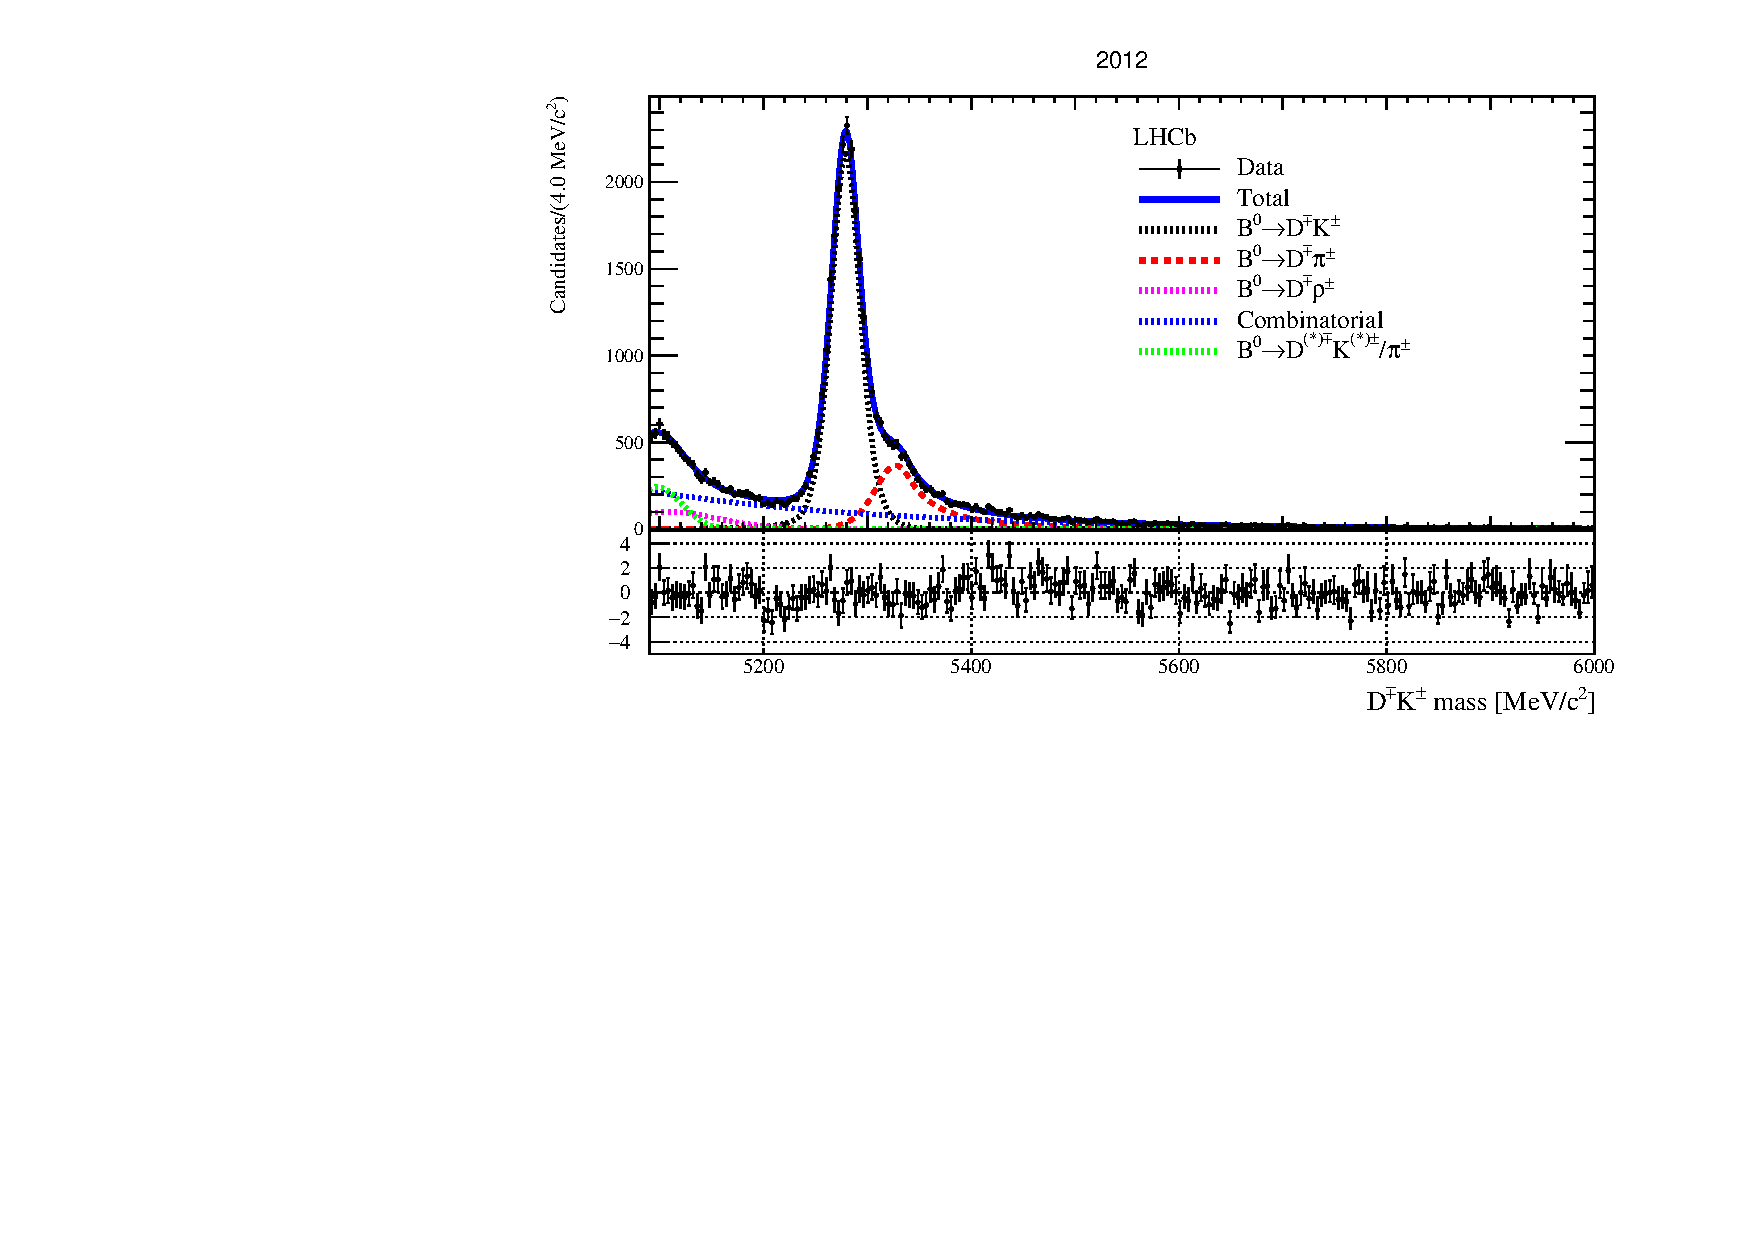
\includegraphics[width=0.48\linewidth]{03Massfit/figs/MDFitPlots_Bd_2012/MDFit_BeautyMass_Bd2DK_withPulls.pdf} \\
		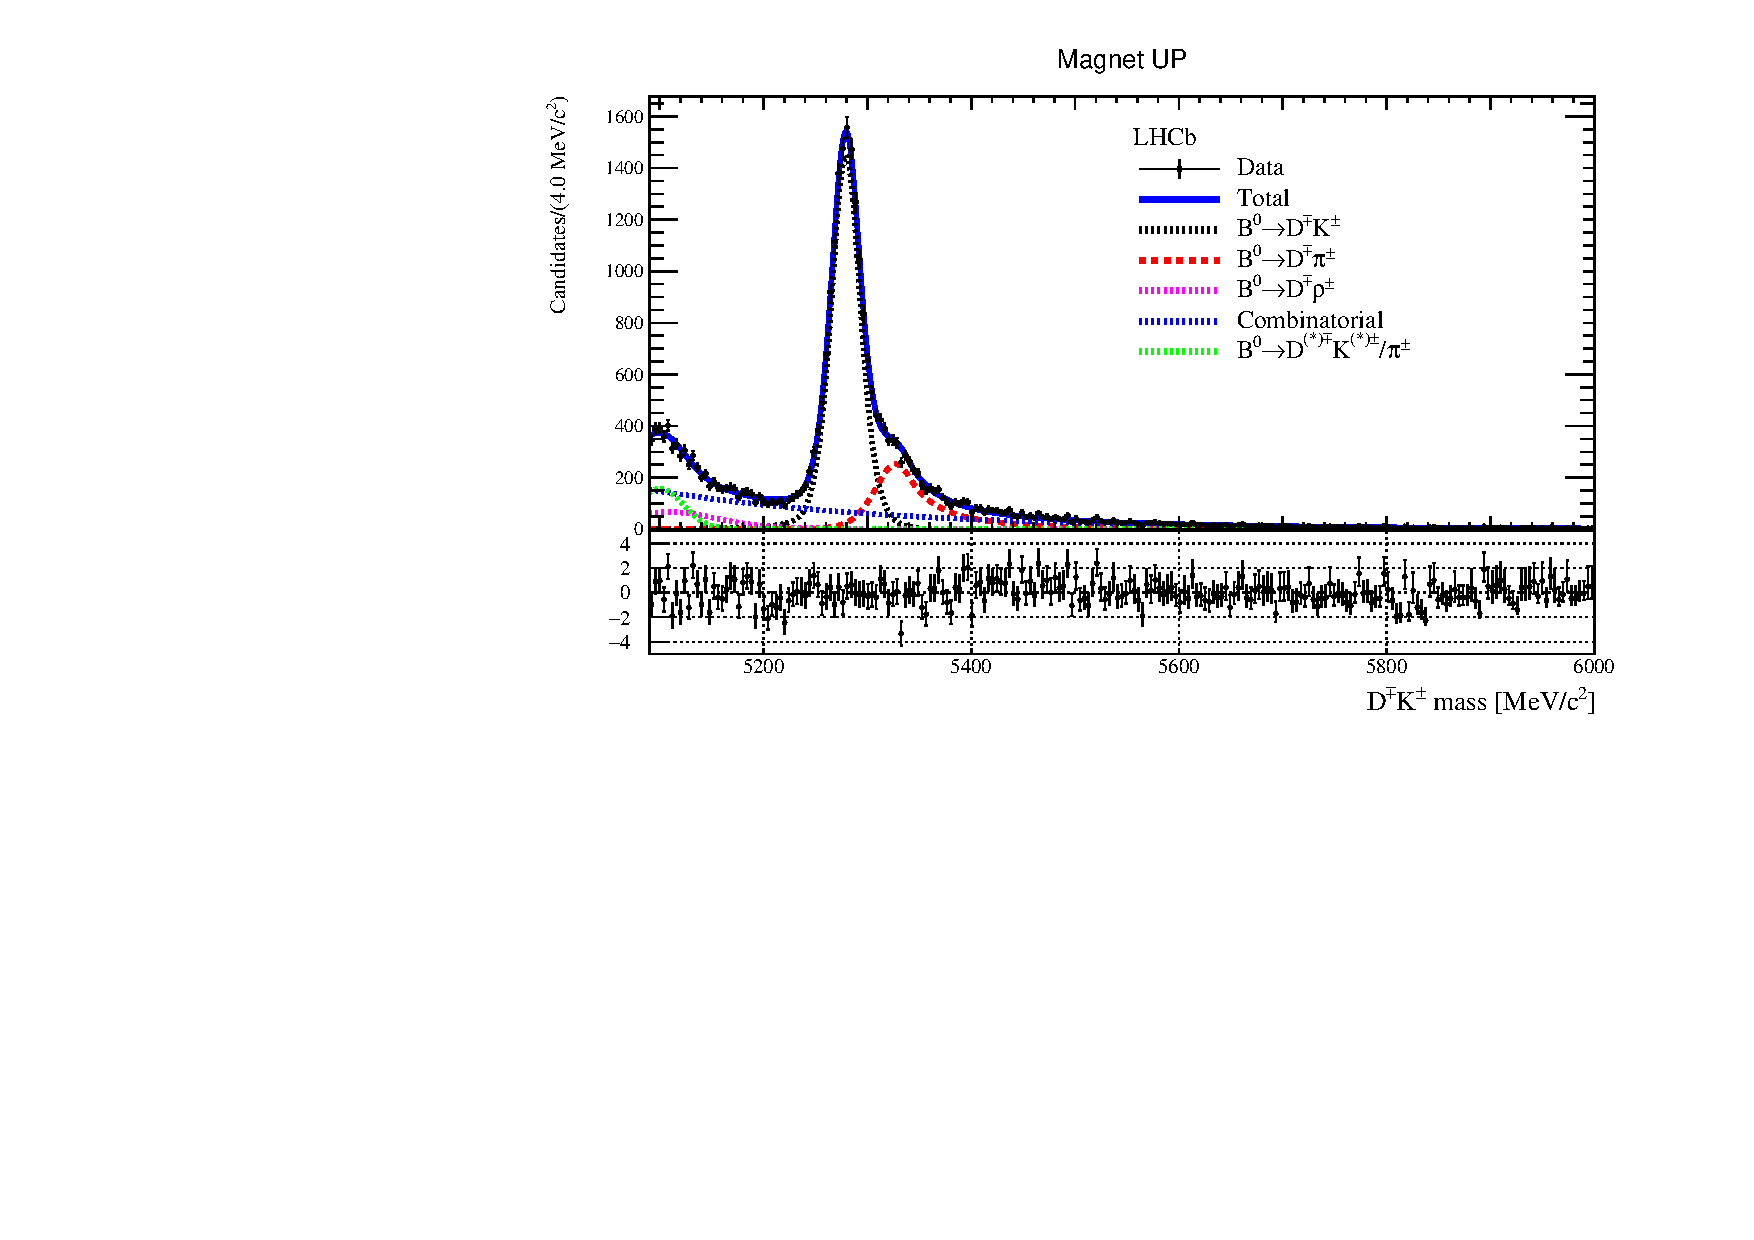
\includegraphics[width=0.48\linewidth]{03Massfit/figs/MDFitPlots_Bd_MU/MDFit_BeautyMass_Bd2DK_withPulls.pdf}
		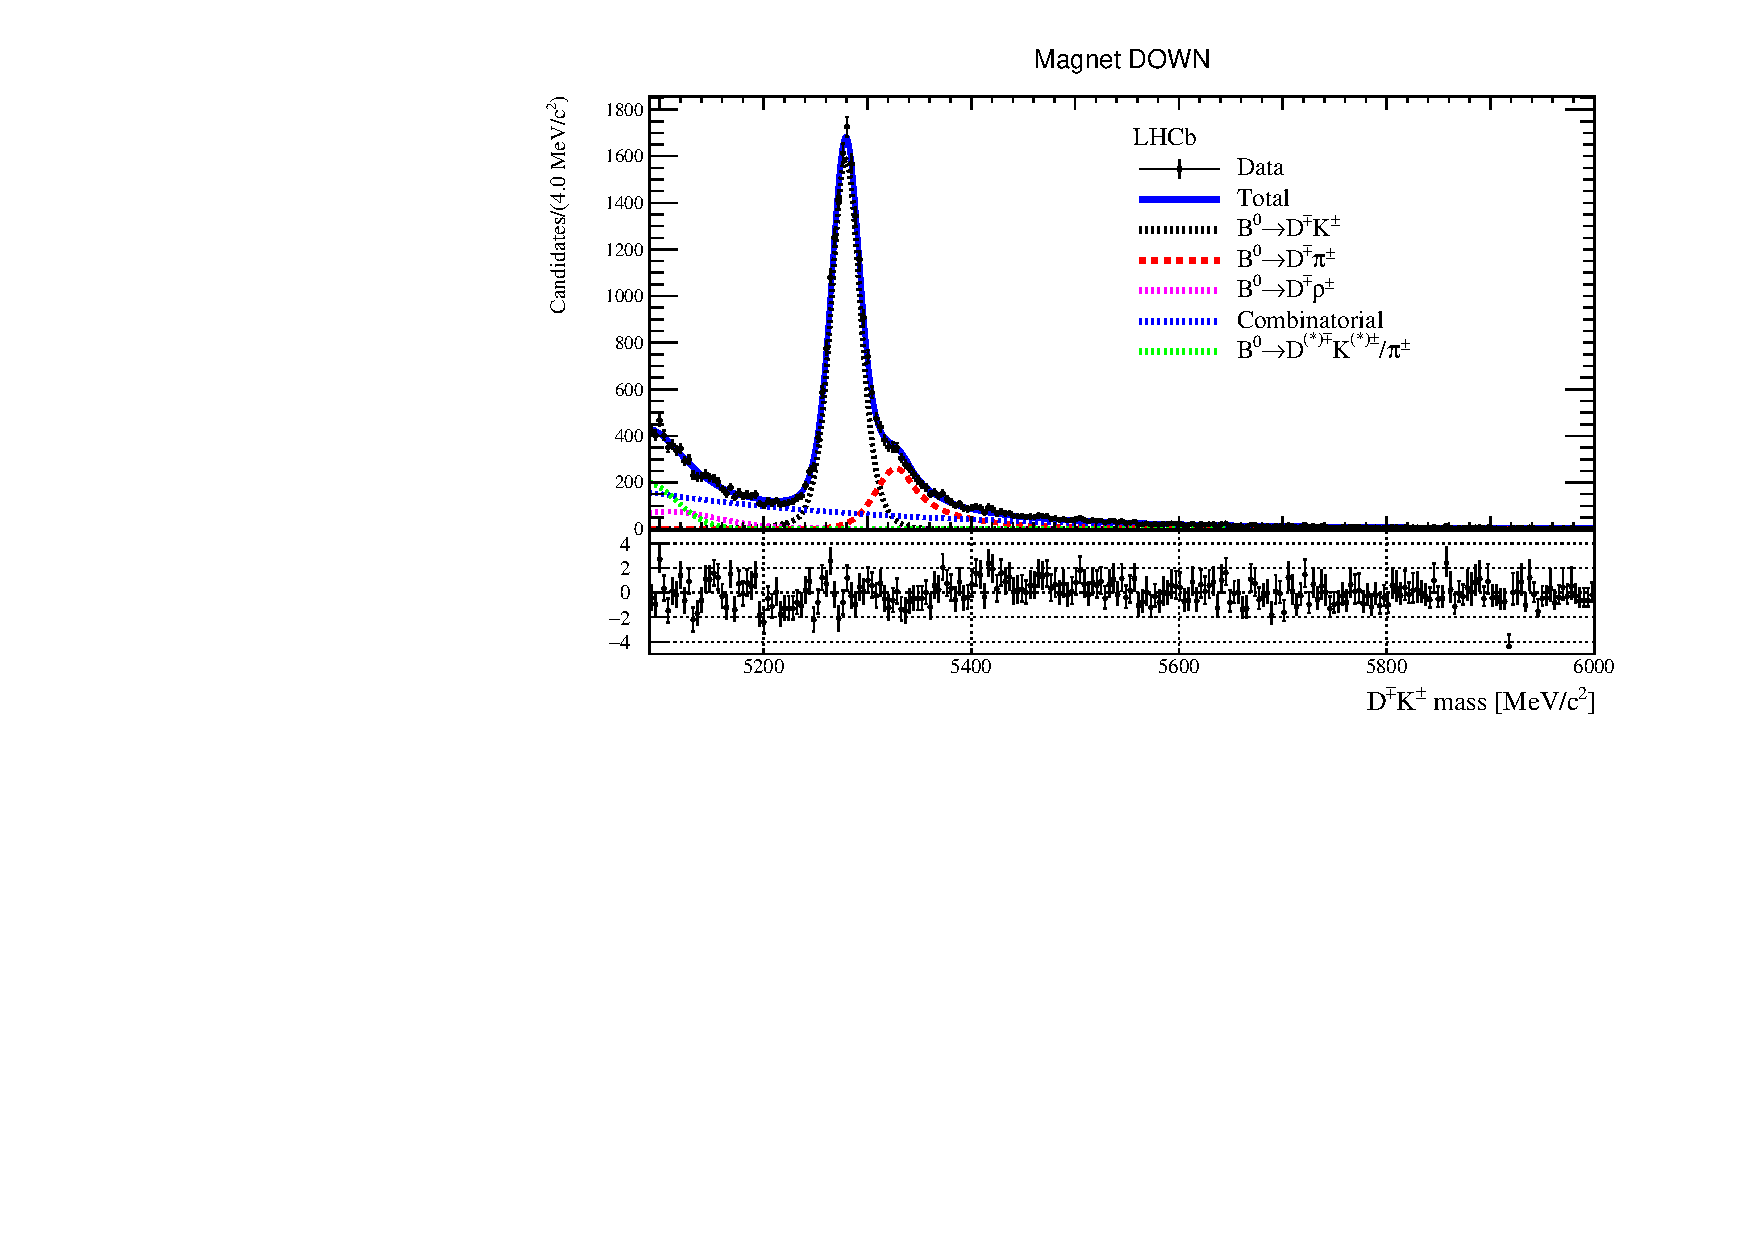
\includegraphics[width=0.48\linewidth]{03Massfit/figs/MDFitPlots_Bd_MD/MDFit_BeautyMass_Bd2DK_withPulls.pdf} \\
		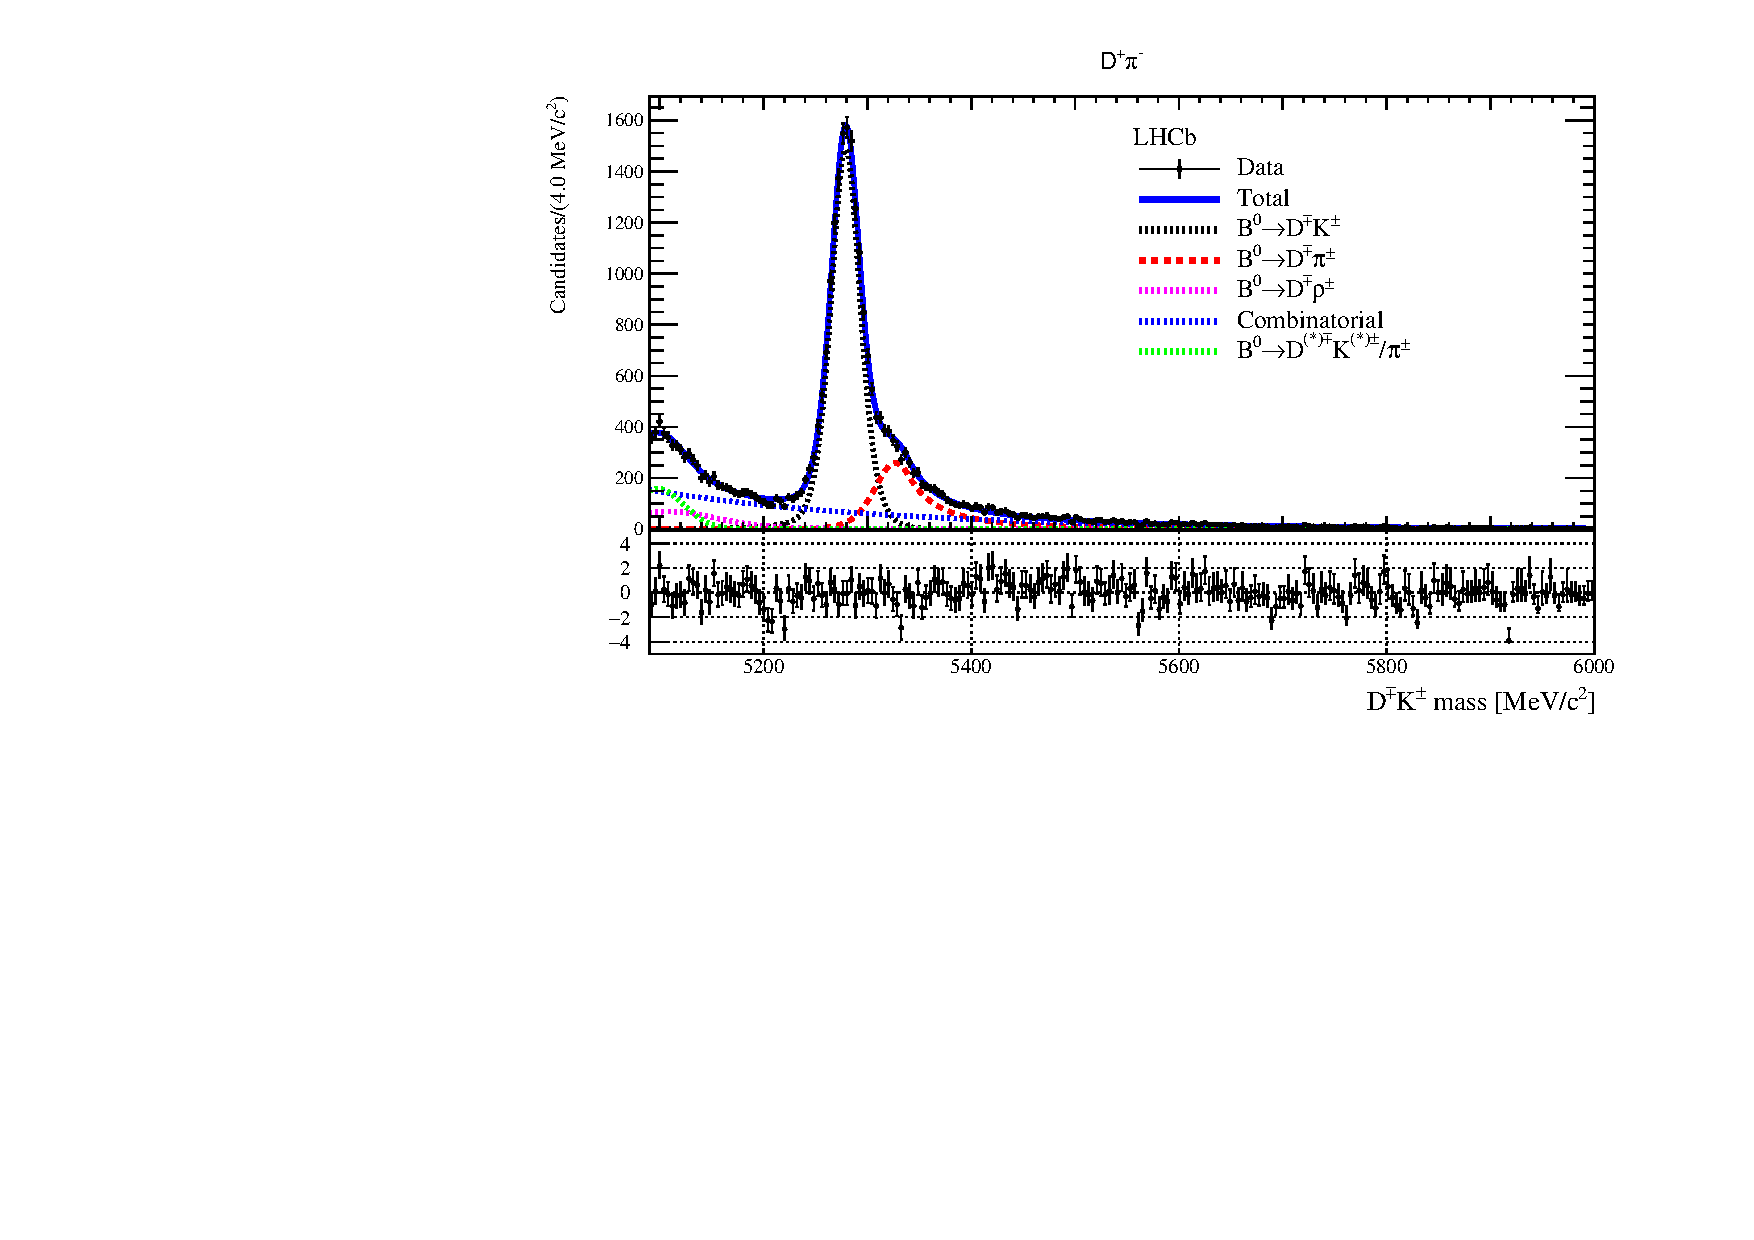
\includegraphics[width=0.48\linewidth]{03Massfit/figs/MDFitPlots_Bd_pim/MDFit_BeautyMass_Bd2DK_withPulls.pdf}
		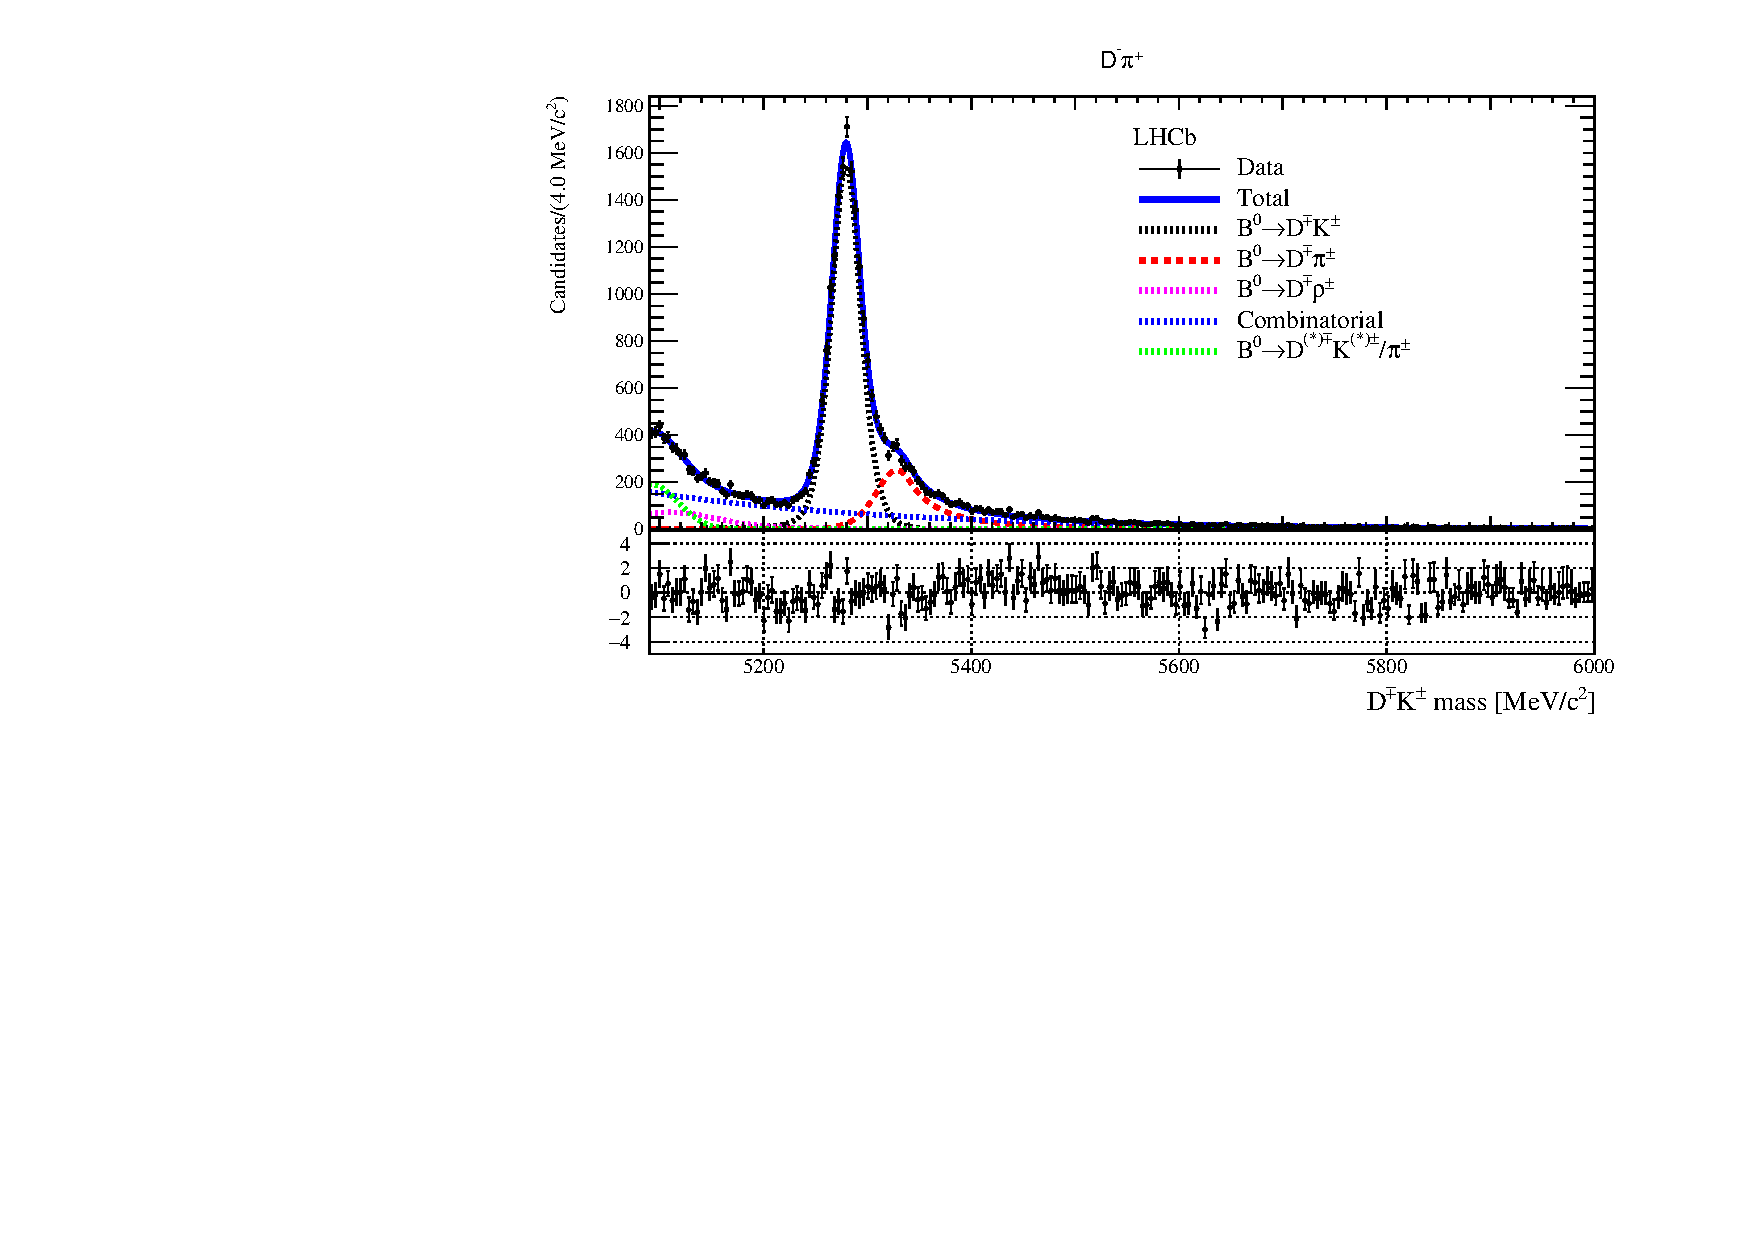
\includegraphics[width=0.48\linewidth]{03Massfit/figs/MDFitPlots_Bd_pip/MDFit_BeautyMass_Bd2DK_withPulls.pdf} \\
		\vspace{-2mm}
                \caption{$\Dmp\Kpm$ mass distributions of the pion sample for each data subsample, with the result of Fit A
                  superimposed.The plots belowthe histograms show thenormalised fit residuals.
		\label{fig:splitfitK}}
	\end{center}
\end{figure}

Fit B strategy is also repeated exactly as before for each subsample. The
corresponding signal and background fitted yields are listed in
Table~\ref{tab:splitted_yields}. The sum of the signal yields for each subsample
is compatible with the signal yield from the fit of total sample (reported in
Table~\ref{tab:FitBfloating}), which is $(4.790\pm0.007)\times10^{5}$.
The asymmetry between the yields of the $\Dm\pip$ and $\Dp\pim$ samples 
is $0.0100\pm0.0015$, which is in agreement with the detection asymmetry between 
$\pip$ and $\pim$ obtained in this analysis and by previous measurements (more details given in Sec.~\ref{sec:datafit}).
The ratio between the fitted yields on the 2011 and 2012 samples is compatible with the different collected luminosities and data taking conditions 
between the two years (twice as much luminosity is collected in 2012 compared to 2011, and the $b$-production cross-section is increased by a factor~$\sim8/7$ in 2012 
because of the increase of the centre-of-mass energy).
Moreover, the ratio of the yields obtained with the magnet up and down samples is in agreement with the ratio of luminosities collected
with the two magnet polarities (same luminosity in 2012, $+30~\%$ more magnet down data in 2011).

\begin{table}[htbp]
        \centering
        \caption{Signal yields (in units of $10^{5}$) in the pion sample for each
                subsample, obtained from Fit B.
        \label{tab:splitted_yields}
        }
        \begin{tabular}{lrr}
                \hline
                2011 & 2012 & Sum \\
                $1.383\pm0.004$ & $3.424\pm0.006$ & $4.807\pm0.007$ \\
                \hline
                Magnet Up & Magnet Down & Sum \\
                $2.263\pm0.005$ & $2.523\pm0.005$ & $4.786\pm0.007$ \\
                \hline
                $\Dm\pip$ & $\Dp\pim$ & Sum \\
                $2.421\pm0.005$ & $2.373\pm0.005$ & $4.794\pm0.007$ \\
                \hline
        \end{tabular}
\end{table}

